\documentclass[twoside]{book}

% Packages required by doxygen
\usepackage{calc}
\usepackage{doxygen}
\usepackage{graphicx}
\usepackage[utf8]{inputenc}
\usepackage{makeidx}
\usepackage{multicol}
\usepackage{multirow}
\usepackage{textcomp}
\usepackage[table]{xcolor}

% Font selection
\usepackage[T1]{fontenc}
\usepackage{mathptmx}
\usepackage[scaled=.90]{helvet}
\usepackage{courier}
\usepackage{amssymb}
\usepackage{sectsty}
\renewcommand{\familydefault}{\sfdefault}
\allsectionsfont{%
  \fontseries{bc}\selectfont%
  \color{darkgray}%
}
\renewcommand{\DoxyLabelFont}{%
  \fontseries{bc}\selectfont%
  \color{darkgray}%
}

% Page & text layout
\usepackage{geometry}
\geometry{%
  a4paper,%
  top=2.5cm,%
  bottom=2.5cm,%
  left=2.5cm,%
  right=2.5cm%
}
\tolerance=750
\hfuzz=15pt
\hbadness=750
\setlength{\emergencystretch}{15pt}
\setlength{\parindent}{0cm}
\setlength{\parskip}{0.2cm}
\makeatletter
\renewcommand{\paragraph}{%
  \@startsection{paragraph}{4}{0ex}{-1.0ex}{1.0ex}{%
    \normalfont\normalsize\bfseries\SS@parafont%
  }%
}
\renewcommand{\subparagraph}{%
  \@startsection{subparagraph}{5}{0ex}{-1.0ex}{1.0ex}{%
    \normalfont\normalsize\bfseries\SS@subparafont%
  }%
}
\makeatother

% Headers & footers
\usepackage{fancyhdr}
\pagestyle{fancyplain}
\fancyhead[LE]{\fancyplain{}{\bfseries\thepage}}
\fancyhead[CE]{\fancyplain{}{}}
\fancyhead[RE]{\fancyplain{}{\bfseries\leftmark}}
\fancyhead[LO]{\fancyplain{}{\bfseries\rightmark}}
\fancyhead[CO]{\fancyplain{}{}}
\fancyhead[RO]{\fancyplain{}{\bfseries\thepage}}
\fancyfoot[LE]{\fancyplain{}{}}
\fancyfoot[CE]{\fancyplain{}{}}
\fancyfoot[RE]{\fancyplain{}{\bfseries\scriptsize Generated on Sun Mar 10 2019 14\-:31\-:22 for Shapes by Doxygen }}
\fancyfoot[LO]{\fancyplain{}{\bfseries\scriptsize Generated on Sun Mar 10 2019 14\-:31\-:22 for Shapes by Doxygen }}
\fancyfoot[CO]{\fancyplain{}{}}
\fancyfoot[RO]{\fancyplain{}{}}
\renewcommand{\footrulewidth}{0.4pt}
\renewcommand{\chaptermark}[1]{%
  \markboth{#1}{}%
}
\renewcommand{\sectionmark}[1]{%
  \markright{\thesection\ #1}%
}

% Indices & bibliography
\usepackage{natbib}
\usepackage[titles]{tocloft}
\setcounter{tocdepth}{3}
\setcounter{secnumdepth}{5}
\makeindex

% Hyperlinks (required, but should be loaded last)
\usepackage{ifpdf}
\ifpdf
  \usepackage[pdftex,pagebackref=true]{hyperref}
\else
  \usepackage[ps2pdf,pagebackref=true]{hyperref}
\fi
\hypersetup{%
  colorlinks=true,%
  linkcolor=blue,%
  citecolor=blue,%
  unicode%
}

% Custom commands
\newcommand{\clearemptydoublepage}{%
  \newpage{\pagestyle{empty}\cleardoublepage}%
}


%===== C O N T E N T S =====

\begin{document}

% Titlepage & ToC
\hypersetup{pageanchor=false}
\pagenumbering{roman}
\begin{titlepage}
\vspace*{7cm}
\begin{center}%
{\Large Shapes \\[1ex]\large 0.\-0.\-1 }\\
\vspace*{1cm}
{\large Generated by Doxygen 1.8.6}\\
\vspace*{0.5cm}
{\small Sun Mar 10 2019 14:31:22}\\
\end{center}
\end{titlepage}
\clearemptydoublepage
\tableofcontents
\clearemptydoublepage
\pagenumbering{arabic}
\hypersetup{pageanchor=true}

%--- Begin generated contents ---
\chapter{Main Page}
\label{index}\hypertarget{index}{}\href{https://travis-ci.org/pavelsimo/shapes}{\tt !\mbox{[}Build Status\mbox{]}(https\-://travis-\/ci.\-org/pavelsimo/shapes.\-svg?branch=master)} \href{https://codecov.io/gh/pavelsimo/shapes}{\tt !\mbox{[}codecov\mbox{]}(https\-://codecov.\-io/gh/pavelsimo/shapes/branch/master/graph/badge.\-svg)} \href{https://github.com/pavelsimo/shapes/blob/master/LICENSE}{\tt !\mbox{[}\mbox{]}(https\-://img.\-shields.\-io/github/license/pavelsimo/shapes.\-svg)}

A lightweight header-\/only planar geometry library for Modern C++


\begin{DoxyItemize}
\item Inspired by python \href{https://pypi.org/project/Shapely/}{\tt shapely}
\item Based on O\-G\-C \href{https://en.wikipedia.org/wiki/Simple_Features}{\tt Simple Features}
\end{DoxyItemize}

\subsection*{Installation}

{\ttfamily shapes} ships as a header-\/only library\-:

```cpp \#include $<$\hyperlink{shapes_8hpp_source}{simo/shapes.\-hpp}$>$

using namespace simo\-::shapes; ```

\subsection*{Examples}

Building a {\ttfamily Point} from Geo\-J\-S\-O\-N\-:

```cpp

auto p = Point\-::from\-\_\-json(R\char`\"{}(\{\char`\"{}type\char`\"{}\-: \char`\"{}Point\char`\"{}, \char`\"{}coordinates\char`\"{}\-: \mbox{[}1.\-0, 2.\-0, 3.\-0\mbox{]}\})\char`\"{}); std\-::cout $<$$<$ p.\-x $<$$<$ \char`\"{} \char`\"{} $<$$<$ p.\-y $<$$<$ \char`\"{} \char`\"{} $<$$<$ p.\-z $<$$<$ std\-::endl; ```

Geo\-J\-S\-O\-N representation of the {\ttfamily Point}\-:

```cpp auto p = Point\{1, 2, 3\}; p.\-precision = 1; std\-::cout $<$$<$ p.\-json() $<$$<$ std\-::endl; ```

```json \{\char`\"{}coordinates\char`\"{}\-:\mbox{[}1.\-0,2.\-0,3.\-0\mbox{]},\char`\"{}type\char`\"{}\-:\char`\"{}\-Point\char`\"{}\} ```

Iterating a {\ttfamily Multi\-Point} is as simple as\-:

```cpp Multi\-Point points(\{\{0, 0, 1\}, \{1, 2, 3\}, \{4, 5, 6\}, \{7, 7, 7\}\}); for(const auto\& point\-: points) \{ std\-::cout $<$$<$ point.\-x $<$$<$ \char`\"{} \char`\"{} $<$$<$ point.\-y $<$$<$ \char`\"{} \char`\"{} $<$$<$ point.\-z $<$$<$ std\-::endl; \} ```

W\-K\-T representation of a {\ttfamily Multi\-Point}\-:

```cpp Multi\-Point points = \{\{1.\-0, 2.\-0, 3.\-0\}, \{4.\-0, 5.\-0, 6.\-0\}\}; points.\-precision = 1; std\-::cout $<$$<$ points.\-wkt() $<$$<$ std\-::endl; ```

``` M\-U\-L\-T\-I\-P\-O\-I\-N\-T\-Z((1.\-0 2.\-0 3.\-0),(4.\-0 5.\-0 6.\-0)) ```

\subsection*{Third-\/party tools}

This project would not have been possible without the following amazing tools, many thanks to its developers!


\begin{DoxyItemize}
\item \href{https://github.com/nlohmann/json}{\tt J\-S\-O\-N for Modern C++}
\item \href{https://github.com/edlund/amalgamate}{\tt amalgamate.\-py}
\item \href{https://github.com/catchorg/Catch2}{\tt Catch2}
\end{DoxyItemize}

\subsection*{License}



\href{http://opensource.org/licenses/MIT}{\tt M\-I\-T License}

Copyright (c) 2019 Pavel Simó

Permission is hereby granted, free of charge, to any person obtaining a copy of this software and associated documentation files (the \char`\"{}\-Software\char`\"{}), to deal in the Software without restriction, including without limitation the rights to use, copy, modify, merge, publish, distribute, sublicense, and/or sell copies of the Software, and to permit persons to whom the Software is furnished to do so, subject to the following conditions\-:

The above copyright notice and this permission notice shall be included in all copies or substantial portions of the Software.

T\-H\-E S\-O\-F\-T\-W\-A\-R\-E I\-S P\-R\-O\-V\-I\-D\-E\-D \char`\"{}\-A\-S I\-S\char`\"{}, W\-I\-T\-H\-O\-U\-T W\-A\-R\-R\-A\-N\-T\-Y O\-F A\-N\-Y K\-I\-N\-D, E\-X\-P\-R\-E\-S\-S O\-R I\-M\-P\-L\-I\-E\-D, I\-N\-C\-L\-U\-D\-I\-N\-G B\-U\-T N\-O\-T L\-I\-M\-I\-T\-E\-D T\-O T\-H\-E W\-A\-R\-R\-A\-N\-T\-I\-E\-S O\-F M\-E\-R\-C\-H\-A\-N\-T\-A\-B\-I\-L\-I\-T\-Y, F\-I\-T\-N\-E\-S\-S F\-O\-R A P\-A\-R\-T\-I\-C\-U\-L\-A\-R P\-U\-R\-P\-O\-S\-E A\-N\-D N\-O\-N\-I\-N\-F\-R\-I\-N\-G\-E\-M\-E\-N\-T. I\-N N\-O E\-V\-E\-N\-T S\-H\-A\-L\-L T\-H\-E A\-U\-T\-H\-O\-R\-S O\-R C\-O\-P\-Y\-R\-I\-G\-H\-T H\-O\-L\-D\-E\-R\-S B\-E L\-I\-A\-B\-L\-E F\-O\-R A\-N\-Y C\-L\-A\-I\-M, D\-A\-M\-A\-G\-E\-S O\-R O\-T\-H\-E\-R L\-I\-A\-B\-I\-L\-I\-T\-Y, W\-H\-E\-T\-H\-E\-R I\-N A\-N A\-C\-T\-I\-O\-N O\-F C\-O\-N\-T\-R\-A\-C\-T, T\-O\-R\-T O\-R O\-T\-H\-E\-R\-W\-I\-S\-E, A\-R\-I\-S\-I\-N\-G F\-R\-O\-M, O\-U\-T O\-F O\-R I\-N C\-O\-N\-N\-E\-C\-T\-I\-O\-N W\-I\-T\-H T\-H\-E S\-O\-F\-T\-W\-A\-R\-E O\-R T\-H\-E U\-S\-E O\-R O\-T\-H\-E\-R D\-E\-A\-L\-I\-N\-G\-S I\-N T\-H\-E S\-O\-F\-T\-W\-A\-R\-E. 
\chapter{Todo List}
\label{todo}
\hypertarget{todo}{}

\begin{DoxyRefList}
\item[\label{todo__todo000002}%
\hypertarget{todo__todo000002}{}%
Class \hyperlink{classsimo_1_1shapes_1_1exceptions_1_1not__implemented__error}{simo\-:\-:shapes\-:\-:exceptions\-:\-:not\-\_\-implemented\-\_\-error} ](pavel) D\-O\-C\-U\-M\-E\-N\-T M\-E!  
\item[\label{todo__todo000001}%
\hypertarget{todo__todo000001}{}%
Class \hyperlink{classsimo_1_1shapes_1_1exceptions_1_1parse__error}{simo\-:\-:shapes\-:\-:exceptions\-:\-:parse\-\_\-error} ](pavel) D\-O\-C\-U\-M\-E\-N\-T M\-E!  
\item[\label{todo__todo000003}%
\hypertarget{todo__todo000003}{}%
Class \hyperlink{classsimo_1_1shapes_1_1exceptions_1_1value__error}{simo\-:\-:shapes\-:\-:exceptions\-:\-:value\-\_\-error} ](pavel) D\-O\-C\-U\-M\-E\-N\-T M\-E!  
\item[\label{todo__todo000006}%
\hypertarget{todo__todo000006}{}%
Member \hyperlink{classsimo_1_1shapes_1_1_multi_point_ad71eee3b464ab12df6e244a63a740e16}{simo\-:\-:shapes\-:\-:Multi\-Point\-:\-:from\-\_\-json} (const std\-::string \&json)](pavel) read properties to specify z, m and zm  
\item[\label{todo__todo000007}%
\hypertarget{todo__todo000007}{}%
Member \hyperlink{classsimo_1_1shapes_1_1_multi_point_af802dae29d3887bec0c6bf3687b4b763}{simo\-:\-:shapes\-:\-:Multi\-Point\-:\-:json} ()](pavel) add properties to specify z, m and zm  
\item[\label{todo__todo000010}%
\hypertarget{todo__todo000010}{}%
Member \hyperlink{classsimo_1_1shapes_1_1_point_a7de22a22436ff219a0714602d865b723}{simo\-:\-:shapes\-:\-:Point\-:\-:from\-\_\-json} (const std\-::string \&json)](pavel) read properties to specify z, m and zm  
\item[\label{todo__todo000011}%
\hypertarget{todo__todo000011}{}%
Member \hyperlink{classsimo_1_1shapes_1_1_point_ab16bf7c8f22a3fbd0df4e8a7407eeda5}{simo\-:\-:shapes\-:\-:Point\-:\-:json} ()](pavel) add properties to specify z, m and zm  
\item[\label{todo__todo000009}%
\hypertarget{todo__todo000009}{}%
Member \hyperlink{classsimo_1_1shapes_1_1_point_aece2f7cb87b1ca009d29fb79fcf8b48a}{simo\-:\-:shapes\-:\-:Point\-:\-:operator!=} (const Point \&other) const ](pavel) D\-O\-C\-U\-M\-E\-N\-T M\-E! 
\begin{DoxyParams}{Parameters}
{\em other} & \\
\hline
\end{DoxyParams}
\begin{DoxyReturn}{Returns}

\end{DoxyReturn}

\item[\label{todo__todo000008}%
\hypertarget{todo__todo000008}{}%
Member \hyperlink{classsimo_1_1shapes_1_1_point_a32b64226c96ab13e4b44e7437c2f6b3e}{simo\-:\-:shapes\-:\-:Point\-:\-:operator==} (const Point \&other) const ](pavel) D\-O\-C\-U\-M\-E\-N\-T M\-E! 
\begin{DoxyParams}{Parameters}
{\em other} & \\
\hline
\end{DoxyParams}
\begin{DoxyReturn}{Returns}

\end{DoxyReturn}

\item[\label{todo__todo000012}%
\hypertarget{todo__todo000012}{}%
Class \hyperlink{classsimo_1_1shapes_1_1_point_collection}{simo\-:\-:shapes\-:\-:Point\-Collection$<$ Derived $>$} ](pavel) add method to get first point 

(pavel) add method to get last point 
\end{DoxyRefList}
\chapter{Hierarchical Index}
\section{Class Hierarchy}
This inheritance list is sorted roughly, but not completely, alphabetically\-:\begin{DoxyCompactList}
\item \contentsline{section}{simo\-:\-:shapes\-:\-:Bounds}{\pageref{classsimo_1_1shapes_1_1_bounds}}{}
\item exception\begin{DoxyCompactList}
\item \contentsline{section}{simo\-:\-:shapes\-:\-:exceptions\-:\-:shapes\-\_\-exception}{\pageref{classsimo_1_1shapes_1_1exceptions_1_1shapes__exception}}{}
\begin{DoxyCompactList}
\item \contentsline{section}{simo\-:\-:shapes\-:\-:exceptions\-:\-:not\-\_\-implemented\-\_\-error}{\pageref{classsimo_1_1shapes_1_1exceptions_1_1not__implemented__error}}{}
\item \contentsline{section}{simo\-:\-:shapes\-:\-:exceptions\-:\-:parse\-\_\-error}{\pageref{classsimo_1_1shapes_1_1exceptions_1_1parse__error}}{}
\item \contentsline{section}{simo\-:\-:shapes\-:\-:exceptions\-:\-:value\-\_\-error}{\pageref{classsimo_1_1shapes_1_1exceptions_1_1value__error}}{}
\end{DoxyCompactList}
\end{DoxyCompactList}
\item \contentsline{section}{simo\-:\-:shapes\-:\-:Geometry}{\pageref{classsimo_1_1shapes_1_1_geometry}}{}
\begin{DoxyCompactList}
\item \contentsline{section}{simo\-:\-:shapes\-:\-:Basic\-Geometry$<$ Linear\-Ring $>$}{\pageref{classsimo_1_1shapes_1_1_basic_geometry}}{}
\begin{DoxyCompactList}
\item \contentsline{section}{simo\-:\-:shapes\-:\-:Linear\-Ring}{\pageref{classsimo_1_1shapes_1_1_linear_ring}}{}
\end{DoxyCompactList}
\item \contentsline{section}{simo\-:\-:shapes\-:\-:Basic\-Geometry$<$ Line\-String $>$}{\pageref{classsimo_1_1shapes_1_1_basic_geometry}}{}
\begin{DoxyCompactList}
\item \contentsline{section}{simo\-:\-:shapes\-:\-:Line\-String}{\pageref{classsimo_1_1shapes_1_1_line_string}}{}
\end{DoxyCompactList}
\item \contentsline{section}{simo\-:\-:shapes\-:\-:Basic\-Geometry$<$ Multi\-Point $>$}{\pageref{classsimo_1_1shapes_1_1_basic_geometry}}{}
\begin{DoxyCompactList}
\item \contentsline{section}{simo\-:\-:shapes\-:\-:Multi\-Point}{\pageref{classsimo_1_1shapes_1_1_multi_point}}{}
\end{DoxyCompactList}
\item \contentsline{section}{simo\-:\-:shapes\-:\-:Basic\-Geometry$<$ Point $>$}{\pageref{classsimo_1_1shapes_1_1_basic_geometry}}{}
\begin{DoxyCompactList}
\item \contentsline{section}{simo\-:\-:shapes\-:\-:Point}{\pageref{classsimo_1_1shapes_1_1_point}}{}
\end{DoxyCompactList}
\item \contentsline{section}{simo\-:\-:shapes\-:\-:Basic\-Geometry$<$ Polygon $>$}{\pageref{classsimo_1_1shapes_1_1_basic_geometry}}{}
\begin{DoxyCompactList}
\item \contentsline{section}{simo\-:\-:shapes\-:\-:Polygon}{\pageref{classsimo_1_1shapes_1_1_polygon}}{}
\end{DoxyCompactList}
\item \contentsline{section}{simo\-:\-:shapes\-:\-:Basic\-Geometry$<$ Derived $>$}{\pageref{classsimo_1_1shapes_1_1_basic_geometry}}{}
\end{DoxyCompactList}
\item \contentsline{section}{simo\-:\-:shapes\-:\-:Point\-Collection$<$ Derived $>$}{\pageref{classsimo_1_1shapes_1_1_point_collection}}{}
\item \contentsline{section}{simo\-:\-:shapes\-:\-:Point\-Collection$<$ Linear\-Ring $>$}{\pageref{classsimo_1_1shapes_1_1_point_collection}}{}
\begin{DoxyCompactList}
\item \contentsline{section}{simo\-:\-:shapes\-:\-:Linear\-Ring}{\pageref{classsimo_1_1shapes_1_1_linear_ring}}{}
\end{DoxyCompactList}
\item \contentsline{section}{simo\-:\-:shapes\-:\-:Point\-Collection$<$ Line\-String $>$}{\pageref{classsimo_1_1shapes_1_1_point_collection}}{}
\begin{DoxyCompactList}
\item \contentsline{section}{simo\-:\-:shapes\-:\-:Line\-String}{\pageref{classsimo_1_1shapes_1_1_line_string}}{}
\end{DoxyCompactList}
\item \contentsline{section}{simo\-:\-:shapes\-:\-:Point\-Collection$<$ Multi\-Point $>$}{\pageref{classsimo_1_1shapes_1_1_point_collection}}{}
\begin{DoxyCompactList}
\item \contentsline{section}{simo\-:\-:shapes\-:\-:Multi\-Point}{\pageref{classsimo_1_1shapes_1_1_multi_point}}{}
\end{DoxyCompactList}
\item \contentsline{section}{simo\-:\-:shapes\-:\-:wkt\-\_\-lexer}{\pageref{classsimo_1_1shapes_1_1wkt__lexer}}{}
\item \contentsline{section}{simo\-:\-:shapes\-:\-:wkt\-\_\-reader}{\pageref{classsimo_1_1shapes_1_1wkt__reader}}{}
\item \contentsline{section}{simo\-:\-:shapes\-:\-:wkt\-\_\-result}{\pageref{structsimo_1_1shapes_1_1wkt__result}}{}
\item \contentsline{section}{Y\-Y\-M\-I\-N\-O\-R\-T\-Y\-P\-E}{\pageref{union_y_y_m_i_n_o_r_t_y_p_e}}{}
\item \contentsline{section}{yy\-Parser}{\pageref{structyy_parser}}{}
\item \contentsline{section}{yy\-Stack\-Entry}{\pageref{structyy_stack_entry}}{}
\end{DoxyCompactList}

\chapter{Class Index}
\section{Class List}
Here are the classes, structs, unions and interfaces with brief descriptions\-:\begin{DoxyCompactList}
\item\contentsline{section}{\hyperlink{classsimo_1_1shapes_1_1_basic_geometry}{simo\-::shapes\-::\-Basic\-Geometry$<$ Derived $>$} \\*Basic geometry type }{\pageref{classsimo_1_1shapes_1_1_basic_geometry}}{}
\item\contentsline{section}{\hyperlink{classsimo_1_1shapes_1_1_bounds}{simo\-::shapes\-::\-Bounds} \\*Bounding box }{\pageref{classsimo_1_1shapes_1_1_bounds}}{}
\item\contentsline{section}{\hyperlink{classsimo_1_1shapes_1_1_geometry}{simo\-::shapes\-::\-Geometry} \\*\hyperlink{classsimo_1_1shapes_1_1_geometry}{Geometry} interface }{\pageref{classsimo_1_1shapes_1_1_geometry}}{}
\item\contentsline{section}{\hyperlink{classsimo_1_1shapes_1_1_linear_ring}{simo\-::shapes\-::\-Linear\-Ring} }{\pageref{classsimo_1_1shapes_1_1_linear_ring}}{}
\item\contentsline{section}{\hyperlink{classsimo_1_1shapes_1_1_line_string}{simo\-::shapes\-::\-Line\-String} }{\pageref{classsimo_1_1shapes_1_1_line_string}}{}
\item\contentsline{section}{\hyperlink{classsimo_1_1shapes_1_1_multi_point}{simo\-::shapes\-::\-Multi\-Point} }{\pageref{classsimo_1_1shapes_1_1_multi_point}}{}
\item\contentsline{section}{\hyperlink{classsimo_1_1shapes_1_1exceptions_1_1not__implemented__error}{simo\-::shapes\-::exceptions\-::not\-\_\-implemented\-\_\-error} }{\pageref{classsimo_1_1shapes_1_1exceptions_1_1not__implemented__error}}{}
\item\contentsline{section}{\hyperlink{classsimo_1_1shapes_1_1exceptions_1_1parse__error}{simo\-::shapes\-::exceptions\-::parse\-\_\-error} }{\pageref{classsimo_1_1shapes_1_1exceptions_1_1parse__error}}{}
\item\contentsline{section}{\hyperlink{classsimo_1_1shapes_1_1_point}{simo\-::shapes\-::\-Point} }{\pageref{classsimo_1_1shapes_1_1_point}}{}
\item\contentsline{section}{\hyperlink{classsimo_1_1shapes_1_1_point_collection}{simo\-::shapes\-::\-Point\-Collection$<$ Derived $>$} }{\pageref{classsimo_1_1shapes_1_1_point_collection}}{}
\item\contentsline{section}{\hyperlink{classsimo_1_1shapes_1_1_polygon}{simo\-::shapes\-::\-Polygon} }{\pageref{classsimo_1_1shapes_1_1_polygon}}{}
\item\contentsline{section}{\hyperlink{classsimo_1_1shapes_1_1exceptions_1_1shapes__exception}{simo\-::shapes\-::exceptions\-::shapes\-\_\-exception} \\*Base shapes exception }{\pageref{classsimo_1_1shapes_1_1exceptions_1_1shapes__exception}}{}
\item\contentsline{section}{\hyperlink{classsimo_1_1shapes_1_1exceptions_1_1value__error}{simo\-::shapes\-::exceptions\-::value\-\_\-error} }{\pageref{classsimo_1_1shapes_1_1exceptions_1_1value__error}}{}
\item\contentsline{section}{\hyperlink{classsimo_1_1shapes_1_1wkt__lexer}{simo\-::shapes\-::wkt\-\_\-lexer} }{\pageref{classsimo_1_1shapes_1_1wkt__lexer}}{}
\item\contentsline{section}{\hyperlink{classsimo_1_1shapes_1_1wkt__reader}{simo\-::shapes\-::wkt\-\_\-reader} }{\pageref{classsimo_1_1shapes_1_1wkt__reader}}{}
\item\contentsline{section}{\hyperlink{structsimo_1_1shapes_1_1wkt__result}{simo\-::shapes\-::wkt\-\_\-result} }{\pageref{structsimo_1_1shapes_1_1wkt__result}}{}
\item\contentsline{section}{\hyperlink{union_y_y_m_i_n_o_r_t_y_p_e}{Y\-Y\-M\-I\-N\-O\-R\-T\-Y\-P\-E} }{\pageref{union_y_y_m_i_n_o_r_t_y_p_e}}{}
\item\contentsline{section}{\hyperlink{structyy_parser}{yy\-Parser} }{\pageref{structyy_parser}}{}
\item\contentsline{section}{\hyperlink{structyy_stack_entry}{yy\-Stack\-Entry} }{\pageref{structyy_stack_entry}}{}
\end{DoxyCompactList}

\chapter{Class Documentation}
\hypertarget{classsimo_1_1shapes_1_1_basic_geometry}{\section{simo\-:\-:shapes\-:\-:Basic\-Geometry$<$ Derived $>$ Class Template Reference}
\label{classsimo_1_1shapes_1_1_basic_geometry}\index{simo\-::shapes\-::\-Basic\-Geometry$<$ Derived $>$@{simo\-::shapes\-::\-Basic\-Geometry$<$ Derived $>$}}
}


basic geometry type  




{\ttfamily \#include $<$geometry.\-hpp$>$}

Inheritance diagram for simo\-:\-:shapes\-:\-:Basic\-Geometry$<$ Derived $>$\-:\begin{figure}[H]
\begin{center}
\leavevmode
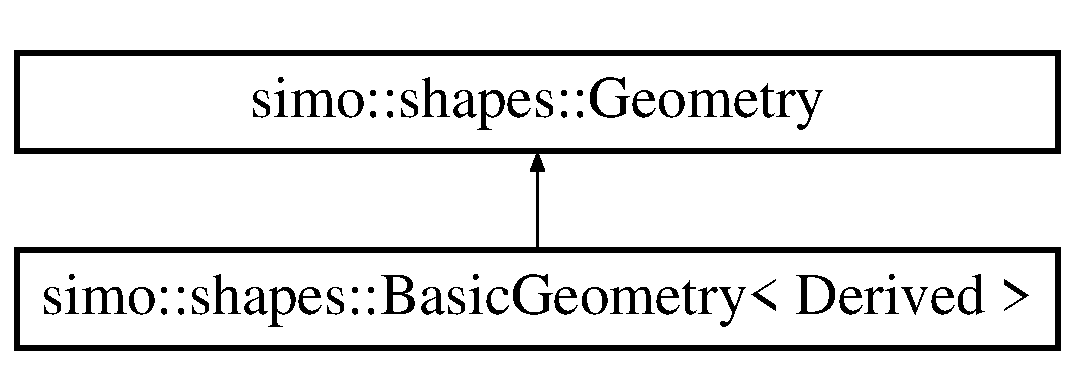
\includegraphics[height=2.000000cm]{classsimo_1_1shapes_1_1_basic_geometry}
\end{center}
\end{figure}
\subsection*{Public Member Functions}
\begin{DoxyCompactItemize}
\item 
Geometry\-Type \hyperlink{classsimo_1_1shapes_1_1_basic_geometry_a8cb2eba04f6fb0cb80cd9c9d2c85f213}{type} () const override
\begin{DoxyCompactList}\small\item\em returns the geometry type (e.\-g. Geometry\-Type\-::\-Point, Geometry\-Type\-::\-Multi\-Point) \end{DoxyCompactList}\item 
Geometry\-Detailed\-Type \hyperlink{classsimo_1_1shapes_1_1_basic_geometry_a82ea146df5c632a15864fc56817d6d0f}{detailed\-\_\-type} () const override
\begin{DoxyCompactList}\small\item\em returns the geometry detailed type (e.\-g. Geometry\-Type\-::\-Point\-Z, Geometry\-Type\-::\-Multi\-Point\-Z\-M) \end{DoxyCompactList}\item 
std\-::string \hyperlink{classsimo_1_1shapes_1_1_basic_geometry_ad2331ba481d41c9f7089787a32ef4ced}{type\-\_\-str} () const override
\begin{DoxyCompactList}\small\item\em returns the geometry type as a string (e.\-g. \hyperlink{classsimo_1_1shapes_1_1_point}{Point}, \hyperlink{classsimo_1_1shapes_1_1_line_string}{Line\-String}) \end{DoxyCompactList}\item 
bool \hyperlink{classsimo_1_1shapes_1_1_basic_geometry_a6834cf02c916d416b84d66d03fa7a525}{empty} () const override
\begin{DoxyCompactList}\small\item\em returns true if the geometry is empty \end{DoxyCompactList}\item 
size\-\_\-t \hyperlink{classsimo_1_1shapes_1_1_basic_geometry_a5e68b783fac81ad8e6c38a0c86875423}{size} () const override
\begin{DoxyCompactList}\small\item\em returns the geometry size \end{DoxyCompactList}\item 
std\-::vector$<$ std\-::tuple\\*
$<$ double, double $>$ $>$ \hyperlink{classsimo_1_1shapes_1_1_basic_geometry_a492b93c475d7a059b4be04a2aafddc99}{xy} () const override
\begin{DoxyCompactList}\small\item\em returns the geometry (x, y) coordinates as a tuple \end{DoxyCompactList}\item 
std\-::vector$<$ std\-::tuple\\*
$<$ double, double, double $>$ $>$ \hyperlink{classsimo_1_1shapes_1_1_basic_geometry_ad0098dca3aab7d3f710d21b672935570}{xyz} () const override
\begin{DoxyCompactList}\small\item\em returns the geometry (x, y, z) coordinates as a tuple \end{DoxyCompactList}\item 
std\-::vector$<$ std\-::tuple\\*
$<$ double, double, double $>$ $>$ \hyperlink{classsimo_1_1shapes_1_1_basic_geometry_ad6f72ade4686897fbea8f3b616b06df8}{xym} () const override
\begin{DoxyCompactList}\small\item\em returns the geometry (x, y, m) coordinates as a tuple \end{DoxyCompactList}\item 
std\-::vector$<$ std\-::tuple\\*
$<$ double, double, double, \\*
double $>$ $>$ \hyperlink{classsimo_1_1shapes_1_1_basic_geometry_a94dd1ee38d7b46ce92d1f547293fedce}{xyzm} () const override
\begin{DoxyCompactList}\small\item\em returns the geometry (x, y, z, m) coordinates as a tuple \end{DoxyCompactList}\item 
Dimension\-Type \hyperlink{classsimo_1_1shapes_1_1_basic_geometry_aa2cf098bf849207e3c1a638a31d28685}{dim} () const override
\begin{DoxyCompactList}\small\item\em returns the dimension type of the geometry \end{DoxyCompactList}\item 
void \hyperlink{classsimo_1_1shapes_1_1_basic_geometry_a203dc3ca9965a82151ec17299a429730}{set\-\_\-dim} (Dimension\-Type value) override
\begin{DoxyCompactList}\small\item\em set the dimension type \end{DoxyCompactList}\item 
\hyperlink{classsimo_1_1shapes_1_1_bounds}{Bounds} \& \hyperlink{classsimo_1_1shapes_1_1_basic_geometry_aef057b58858f64a47a8fa68b7a9ef7d1}{bounds} () override
\begin{DoxyCompactList}\small\item\em returns the geometry bounds \end{DoxyCompactList}\item 
bool \hyperlink{classsimo_1_1shapes_1_1_basic_geometry_adf922693df08f41d170438836bc90c6b}{has\-\_\-z} () const override
\begin{DoxyCompactList}\small\item\em whether the geometry has z-\/coordinate \end{DoxyCompactList}\item 
bool \hyperlink{classsimo_1_1shapes_1_1_basic_geometry_ae67e31810708aa668749f1d1ae8ae28b}{has\-\_\-m} () const override
\begin{DoxyCompactList}\small\item\em whether the geometry has m-\/coordinate \end{DoxyCompactList}\item 
bool \hyperlink{classsimo_1_1shapes_1_1_basic_geometry_ae5ad57479626834ef3c4e10c2fb2275b}{is\-\_\-closed} () const override
\begin{DoxyCompactList}\small\item\em whether the geometry is closed \end{DoxyCompactList}\item 
int8\-\_\-t \hyperlink{classsimo_1_1shapes_1_1_basic_geometry_ae5ae8173a8c166d98ddda0fbfbc48346}{ndim} () const override
\begin{DoxyCompactList}\small\item\em returns the number of dimensions of the geometry \end{DoxyCompactList}\end{DoxyCompactItemize}
\subsection*{Public Attributes}
\begin{DoxyCompactItemize}
\item 
\hypertarget{classsimo_1_1shapes_1_1_basic_geometry_ae4429e3d4c999289a0d7ae706e6ddcf7}{int8\-\_\-t \hyperlink{classsimo_1_1shapes_1_1_basic_geometry_ae4429e3d4c999289a0d7ae706e6ddcf7}{precision} = 1}\label{classsimo_1_1shapes_1_1_basic_geometry_ae4429e3d4c999289a0d7ae706e6ddcf7}

\begin{DoxyCompactList}\small\item\em serialization precision \end{DoxyCompactList}\item 
\hypertarget{classsimo_1_1shapes_1_1_basic_geometry_aaf510a85f9f8ec7160637c73f88b2c6a}{int32\-\_\-t \hyperlink{classsimo_1_1shapes_1_1_basic_geometry_aaf510a85f9f8ec7160637c73f88b2c6a}{srid} = -\/1}\label{classsimo_1_1shapes_1_1_basic_geometry_aaf510a85f9f8ec7160637c73f88b2c6a}

\begin{DoxyCompactList}\small\item\em a spatial reference identifier (S\-R\-I\-D) is a unique identifier associated with a specific coordinate system \end{DoxyCompactList}\end{DoxyCompactItemize}


\subsection{Detailed Description}
\subsubsection*{template$<$typename Derived$>$class simo\-::shapes\-::\-Basic\-Geometry$<$ Derived $>$}

basic geometry type 

Definition at line 160 of file geometry.\-hpp.



\subsection{Member Function Documentation}
\hypertarget{classsimo_1_1shapes_1_1_basic_geometry_aef057b58858f64a47a8fa68b7a9ef7d1}{\index{simo\-::shapes\-::\-Basic\-Geometry@{simo\-::shapes\-::\-Basic\-Geometry}!bounds@{bounds}}
\index{bounds@{bounds}!simo::shapes::BasicGeometry@{simo\-::shapes\-::\-Basic\-Geometry}}
\subsubsection[{bounds}]{\setlength{\rightskip}{0pt plus 5cm}template$<$typename Derived$>$ {\bf Bounds}\& {\bf simo\-::shapes\-::\-Basic\-Geometry}$<$ Derived $>$\-::bounds (
\begin{DoxyParamCaption}
{}
\end{DoxyParamCaption}
)\hspace{0.3cm}{\ttfamily [inline]}, {\ttfamily [override]}, {\ttfamily [virtual]}}}\label{classsimo_1_1shapes_1_1_basic_geometry_aef057b58858f64a47a8fa68b7a9ef7d1}


returns the geometry bounds 

\begin{DoxyReturn}{Returns}
the geometry bounds
\end{DoxyReturn}
\begin{DoxySince}{Since}
0.\-0.\-1 
\end{DoxySince}


Implements \hyperlink{classsimo_1_1shapes_1_1_geometry_a0ed6566c6f79af7255f5950bd44f2a1e}{simo\-::shapes\-::\-Geometry}.



Definition at line 388 of file geometry.\-hpp.

\hypertarget{classsimo_1_1shapes_1_1_basic_geometry_a82ea146df5c632a15864fc56817d6d0f}{\index{simo\-::shapes\-::\-Basic\-Geometry@{simo\-::shapes\-::\-Basic\-Geometry}!detailed\-\_\-type@{detailed\-\_\-type}}
\index{detailed\-\_\-type@{detailed\-\_\-type}!simo::shapes::BasicGeometry@{simo\-::shapes\-::\-Basic\-Geometry}}
\subsubsection[{detailed\-\_\-type}]{\setlength{\rightskip}{0pt plus 5cm}template$<$typename Derived$>$ Geometry\-Detailed\-Type {\bf simo\-::shapes\-::\-Basic\-Geometry}$<$ Derived $>$\-::detailed\-\_\-type (
\begin{DoxyParamCaption}
{}
\end{DoxyParamCaption}
) const\hspace{0.3cm}{\ttfamily [inline]}, {\ttfamily [override]}, {\ttfamily [virtual]}}}\label{classsimo_1_1shapes_1_1_basic_geometry_a82ea146df5c632a15864fc56817d6d0f}


returns the geometry detailed type (e.\-g. Geometry\-Type\-::\-Point\-Z, Geometry\-Type\-::\-Multi\-Point\-Z\-M) 

\begin{DoxyReturn}{Returns}
the geometry detailed type
\end{DoxyReturn}
\begin{DoxySince}{Since}
0.\-0.\-1 
\end{DoxySince}


Implements \hyperlink{classsimo_1_1shapes_1_1_geometry_a5633ca34213554220aa19257260b2211}{simo\-::shapes\-::\-Geometry}.



Definition at line 174 of file geometry.\-hpp.

\hypertarget{classsimo_1_1shapes_1_1_basic_geometry_aa2cf098bf849207e3c1a638a31d28685}{\index{simo\-::shapes\-::\-Basic\-Geometry@{simo\-::shapes\-::\-Basic\-Geometry}!dim@{dim}}
\index{dim@{dim}!simo::shapes::BasicGeometry@{simo\-::shapes\-::\-Basic\-Geometry}}
\subsubsection[{dim}]{\setlength{\rightskip}{0pt plus 5cm}template$<$typename Derived$>$ Dimension\-Type {\bf simo\-::shapes\-::\-Basic\-Geometry}$<$ Derived $>$\-::dim (
\begin{DoxyParamCaption}
{}
\end{DoxyParamCaption}
) const\hspace{0.3cm}{\ttfamily [inline]}, {\ttfamily [override]}, {\ttfamily [virtual]}}}\label{classsimo_1_1shapes_1_1_basic_geometry_aa2cf098bf849207e3c1a638a31d28685}


returns the dimension type of the geometry 

\begin{DoxyReturn}{Returns}
the dimension type
\end{DoxyReturn}
\begin{DoxyNote}{Note}
the dimension type is (x, y), (x, y, z), (x, y, m) and (x, y, z, m)
\end{DoxyNote}
\begin{DoxySince}{Since}
0.\-0.\-1 
\end{DoxySince}


Implements \hyperlink{classsimo_1_1shapes_1_1_geometry_a8db862418cec85fc52c832267449d392}{simo\-::shapes\-::\-Geometry}.



Definition at line 378 of file geometry.\-hpp.

\hypertarget{classsimo_1_1shapes_1_1_basic_geometry_a6834cf02c916d416b84d66d03fa7a525}{\index{simo\-::shapes\-::\-Basic\-Geometry@{simo\-::shapes\-::\-Basic\-Geometry}!empty@{empty}}
\index{empty@{empty}!simo::shapes::BasicGeometry@{simo\-::shapes\-::\-Basic\-Geometry}}
\subsubsection[{empty}]{\setlength{\rightskip}{0pt plus 5cm}template$<$typename Derived$>$ bool {\bf simo\-::shapes\-::\-Basic\-Geometry}$<$ Derived $>$\-::empty (
\begin{DoxyParamCaption}
{}
\end{DoxyParamCaption}
) const\hspace{0.3cm}{\ttfamily [inline]}, {\ttfamily [override]}, {\ttfamily [virtual]}}}\label{classsimo_1_1shapes_1_1_basic_geometry_a6834cf02c916d416b84d66d03fa7a525}


returns true if the geometry is empty 

\begin{DoxyReturn}{Returns}
true if the the geometry is empty, otherwise false
\end{DoxyReturn}
\begin{DoxySince}{Since}
0.\-0.\-1 
\end{DoxySince}


Implements \hyperlink{classsimo_1_1shapes_1_1_geometry_ab53733864d430504fd7ed2b564c96ef5}{simo\-::shapes\-::\-Geometry}.



Definition at line 348 of file geometry.\-hpp.

\hypertarget{classsimo_1_1shapes_1_1_basic_geometry_ae67e31810708aa668749f1d1ae8ae28b}{\index{simo\-::shapes\-::\-Basic\-Geometry@{simo\-::shapes\-::\-Basic\-Geometry}!has\-\_\-m@{has\-\_\-m}}
\index{has\-\_\-m@{has\-\_\-m}!simo::shapes::BasicGeometry@{simo\-::shapes\-::\-Basic\-Geometry}}
\subsubsection[{has\-\_\-m}]{\setlength{\rightskip}{0pt plus 5cm}template$<$typename Derived$>$ bool {\bf simo\-::shapes\-::\-Basic\-Geometry}$<$ Derived $>$\-::has\-\_\-m (
\begin{DoxyParamCaption}
{}
\end{DoxyParamCaption}
) const\hspace{0.3cm}{\ttfamily [inline]}, {\ttfamily [override]}, {\ttfamily [virtual]}}}\label{classsimo_1_1shapes_1_1_basic_geometry_ae67e31810708aa668749f1d1ae8ae28b}


whether the geometry has m-\/coordinate 

\begin{DoxyReturn}{Returns}
true if the geometry has m-\/coordinate, otherwise false
\end{DoxyReturn}
\begin{DoxySince}{Since}
0.\-0.\-1 
\end{DoxySince}


Implements \hyperlink{classsimo_1_1shapes_1_1_geometry_aa6b0b9e19c782d137effc7be2e5416a1}{simo\-::shapes\-::\-Geometry}.



Definition at line 398 of file geometry.\-hpp.

\hypertarget{classsimo_1_1shapes_1_1_basic_geometry_adf922693df08f41d170438836bc90c6b}{\index{simo\-::shapes\-::\-Basic\-Geometry@{simo\-::shapes\-::\-Basic\-Geometry}!has\-\_\-z@{has\-\_\-z}}
\index{has\-\_\-z@{has\-\_\-z}!simo::shapes::BasicGeometry@{simo\-::shapes\-::\-Basic\-Geometry}}
\subsubsection[{has\-\_\-z}]{\setlength{\rightskip}{0pt plus 5cm}template$<$typename Derived$>$ bool {\bf simo\-::shapes\-::\-Basic\-Geometry}$<$ Derived $>$\-::has\-\_\-z (
\begin{DoxyParamCaption}
{}
\end{DoxyParamCaption}
) const\hspace{0.3cm}{\ttfamily [inline]}, {\ttfamily [override]}, {\ttfamily [virtual]}}}\label{classsimo_1_1shapes_1_1_basic_geometry_adf922693df08f41d170438836bc90c6b}


whether the geometry has z-\/coordinate 

\begin{DoxyReturn}{Returns}
true if the geometry has z-\/coordinate, otherwise false
\end{DoxyReturn}
\begin{DoxySince}{Since}
0.\-0.\-1 
\end{DoxySince}


Implements \hyperlink{classsimo_1_1shapes_1_1_geometry_a7d2d67f5845bcccca7d88619b0be288a}{simo\-::shapes\-::\-Geometry}.



Definition at line 393 of file geometry.\-hpp.

\hypertarget{classsimo_1_1shapes_1_1_basic_geometry_ae5ad57479626834ef3c4e10c2fb2275b}{\index{simo\-::shapes\-::\-Basic\-Geometry@{simo\-::shapes\-::\-Basic\-Geometry}!is\-\_\-closed@{is\-\_\-closed}}
\index{is\-\_\-closed@{is\-\_\-closed}!simo::shapes::BasicGeometry@{simo\-::shapes\-::\-Basic\-Geometry}}
\subsubsection[{is\-\_\-closed}]{\setlength{\rightskip}{0pt plus 5cm}template$<$typename Derived$>$ bool {\bf simo\-::shapes\-::\-Basic\-Geometry}$<$ Derived $>$\-::is\-\_\-closed (
\begin{DoxyParamCaption}
{}
\end{DoxyParamCaption}
) const\hspace{0.3cm}{\ttfamily [inline]}, {\ttfamily [override]}, {\ttfamily [virtual]}}}\label{classsimo_1_1shapes_1_1_basic_geometry_ae5ad57479626834ef3c4e10c2fb2275b}


whether the geometry is closed 

\begin{DoxyReturn}{Returns}
true if the geometry is closed, otherwise false
\end{DoxyReturn}
\begin{DoxySince}{Since}
0.\-0.\-1 
\end{DoxySince}


Implements \hyperlink{classsimo_1_1shapes_1_1_geometry_a2c1ea77c6f3b7b6c20eb9894be264f80}{simo\-::shapes\-::\-Geometry}.



Definition at line 403 of file geometry.\-hpp.

\hypertarget{classsimo_1_1shapes_1_1_basic_geometry_ae5ae8173a8c166d98ddda0fbfbc48346}{\index{simo\-::shapes\-::\-Basic\-Geometry@{simo\-::shapes\-::\-Basic\-Geometry}!ndim@{ndim}}
\index{ndim@{ndim}!simo::shapes::BasicGeometry@{simo\-::shapes\-::\-Basic\-Geometry}}
\subsubsection[{ndim}]{\setlength{\rightskip}{0pt plus 5cm}template$<$typename Derived$>$ int8\-\_\-t {\bf simo\-::shapes\-::\-Basic\-Geometry}$<$ Derived $>$\-::ndim (
\begin{DoxyParamCaption}
{}
\end{DoxyParamCaption}
) const\hspace{0.3cm}{\ttfamily [inline]}, {\ttfamily [override]}, {\ttfamily [virtual]}}}\label{classsimo_1_1shapes_1_1_basic_geometry_ae5ae8173a8c166d98ddda0fbfbc48346}


returns the number of dimensions of the geometry 

\begin{DoxyReturn}{Returns}
the number of dimensions
\end{DoxyReturn}
\begin{DoxyNote}{Note}
the number of dimensions is (x, y) = 2, (x, y, z) = 3, (x, y, m) = 3 and (x, y, z, m) = 4
\end{DoxyNote}
\begin{DoxySince}{Since}
0.\-0.\-1 
\end{DoxySince}


Implements \hyperlink{classsimo_1_1shapes_1_1_geometry_ab4890550ac2208165a5953a989d0b2aa}{simo\-::shapes\-::\-Geometry}.



Definition at line 408 of file geometry.\-hpp.

\hypertarget{classsimo_1_1shapes_1_1_basic_geometry_a203dc3ca9965a82151ec17299a429730}{\index{simo\-::shapes\-::\-Basic\-Geometry@{simo\-::shapes\-::\-Basic\-Geometry}!set\-\_\-dim@{set\-\_\-dim}}
\index{set\-\_\-dim@{set\-\_\-dim}!simo::shapes::BasicGeometry@{simo\-::shapes\-::\-Basic\-Geometry}}
\subsubsection[{set\-\_\-dim}]{\setlength{\rightskip}{0pt plus 5cm}template$<$typename Derived$>$ void {\bf simo\-::shapes\-::\-Basic\-Geometry}$<$ Derived $>$\-::set\-\_\-dim (
\begin{DoxyParamCaption}
\item[{Dimension\-Type}]{value}
\end{DoxyParamCaption}
)\hspace{0.3cm}{\ttfamily [inline]}, {\ttfamily [override]}, {\ttfamily [virtual]}}}\label{classsimo_1_1shapes_1_1_basic_geometry_a203dc3ca9965a82151ec17299a429730}


set the dimension type 


\begin{DoxyParams}{Parameters}
{\em value} & the dimension type\\
\hline
\end{DoxyParams}
\begin{DoxySince}{Since}
0.\-0.\-1 
\end{DoxySince}


Implements \hyperlink{classsimo_1_1shapes_1_1_geometry_adbd7a14a8b4414c882cbcafa8025085d}{simo\-::shapes\-::\-Geometry}.



Definition at line 383 of file geometry.\-hpp.

\hypertarget{classsimo_1_1shapes_1_1_basic_geometry_a5e68b783fac81ad8e6c38a0c86875423}{\index{simo\-::shapes\-::\-Basic\-Geometry@{simo\-::shapes\-::\-Basic\-Geometry}!size@{size}}
\index{size@{size}!simo::shapes::BasicGeometry@{simo\-::shapes\-::\-Basic\-Geometry}}
\subsubsection[{size}]{\setlength{\rightskip}{0pt plus 5cm}template$<$typename Derived$>$ size\-\_\-t {\bf simo\-::shapes\-::\-Basic\-Geometry}$<$ Derived $>$\-::size (
\begin{DoxyParamCaption}
{}
\end{DoxyParamCaption}
) const\hspace{0.3cm}{\ttfamily [inline]}, {\ttfamily [override]}, {\ttfamily [virtual]}}}\label{classsimo_1_1shapes_1_1_basic_geometry_a5e68b783fac81ad8e6c38a0c86875423}


returns the geometry size 

\begin{DoxyReturn}{Returns}
the size of the geometry
\end{DoxyReturn}
\begin{DoxySince}{Since}
0.\-0.\-1 
\end{DoxySince}


Implements \hyperlink{classsimo_1_1shapes_1_1_geometry_a110e8a897b84c704f9009679bbbe21fc}{simo\-::shapes\-::\-Geometry}.



Definition at line 353 of file geometry.\-hpp.

\hypertarget{classsimo_1_1shapes_1_1_basic_geometry_a8cb2eba04f6fb0cb80cd9c9d2c85f213}{\index{simo\-::shapes\-::\-Basic\-Geometry@{simo\-::shapes\-::\-Basic\-Geometry}!type@{type}}
\index{type@{type}!simo::shapes::BasicGeometry@{simo\-::shapes\-::\-Basic\-Geometry}}
\subsubsection[{type}]{\setlength{\rightskip}{0pt plus 5cm}template$<$typename Derived$>$ Geometry\-Type {\bf simo\-::shapes\-::\-Basic\-Geometry}$<$ Derived $>$\-::type (
\begin{DoxyParamCaption}
{}
\end{DoxyParamCaption}
) const\hspace{0.3cm}{\ttfamily [inline]}, {\ttfamily [override]}, {\ttfamily [virtual]}}}\label{classsimo_1_1shapes_1_1_basic_geometry_a8cb2eba04f6fb0cb80cd9c9d2c85f213}


returns the geometry type (e.\-g. Geometry\-Type\-::\-Point, Geometry\-Type\-::\-Multi\-Point) 

\begin{DoxyReturn}{Returns}
the geometry type
\end{DoxyReturn}
\begin{DoxySince}{Since}
0.\-0.\-1 
\end{DoxySince}


Implements \hyperlink{classsimo_1_1shapes_1_1_geometry_a97a21e31df877cd74da81e08e6e1c7ff}{simo\-::shapes\-::\-Geometry}.



Definition at line 169 of file geometry.\-hpp.

\hypertarget{classsimo_1_1shapes_1_1_basic_geometry_ad2331ba481d41c9f7089787a32ef4ced}{\index{simo\-::shapes\-::\-Basic\-Geometry@{simo\-::shapes\-::\-Basic\-Geometry}!type\-\_\-str@{type\-\_\-str}}
\index{type\-\_\-str@{type\-\_\-str}!simo::shapes::BasicGeometry@{simo\-::shapes\-::\-Basic\-Geometry}}
\subsubsection[{type\-\_\-str}]{\setlength{\rightskip}{0pt plus 5cm}template$<$typename Derived$>$ std\-::string {\bf simo\-::shapes\-::\-Basic\-Geometry}$<$ Derived $>$\-::type\-\_\-str (
\begin{DoxyParamCaption}
{}
\end{DoxyParamCaption}
) const\hspace{0.3cm}{\ttfamily [inline]}, {\ttfamily [override]}, {\ttfamily [virtual]}}}\label{classsimo_1_1shapes_1_1_basic_geometry_ad2331ba481d41c9f7089787a32ef4ced}


returns the geometry type as a string (e.\-g. \hyperlink{classsimo_1_1shapes_1_1_point}{Point}, \hyperlink{classsimo_1_1shapes_1_1_line_string}{Line\-String}) 

\begin{DoxyReturn}{Returns}
the geometry type as a string
\end{DoxyReturn}
\begin{DoxySince}{Since}
0.\-0.\-1 
\end{DoxySince}


Implements \hyperlink{classsimo_1_1shapes_1_1_geometry_aa4fc3ffa8fa908f238c2917166a4f0a1}{simo\-::shapes\-::\-Geometry}.



Definition at line 343 of file geometry.\-hpp.

\hypertarget{classsimo_1_1shapes_1_1_basic_geometry_a492b93c475d7a059b4be04a2aafddc99}{\index{simo\-::shapes\-::\-Basic\-Geometry@{simo\-::shapes\-::\-Basic\-Geometry}!xy@{xy}}
\index{xy@{xy}!simo::shapes::BasicGeometry@{simo\-::shapes\-::\-Basic\-Geometry}}
\subsubsection[{xy}]{\setlength{\rightskip}{0pt plus 5cm}template$<$typename Derived$>$ std\-::vector$<$std\-::tuple$<$double, double$>$ $>$ {\bf simo\-::shapes\-::\-Basic\-Geometry}$<$ Derived $>$\-::xy (
\begin{DoxyParamCaption}
{}
\end{DoxyParamCaption}
) const\hspace{0.3cm}{\ttfamily [inline]}, {\ttfamily [override]}, {\ttfamily [virtual]}}}\label{classsimo_1_1shapes_1_1_basic_geometry_a492b93c475d7a059b4be04a2aafddc99}


returns the geometry (x, y) coordinates as a tuple 

\begin{DoxyReturn}{Returns}
a vector of (x, y) tuples
\end{DoxyReturn}
\begin{DoxySince}{Since}
0.\-0.\-1 
\end{DoxySince}


Implements \hyperlink{classsimo_1_1shapes_1_1_geometry_aa45dedcadd8e44be1f9415223ca2e19d}{simo\-::shapes\-::\-Geometry}.



Definition at line 358 of file geometry.\-hpp.

\hypertarget{classsimo_1_1shapes_1_1_basic_geometry_ad6f72ade4686897fbea8f3b616b06df8}{\index{simo\-::shapes\-::\-Basic\-Geometry@{simo\-::shapes\-::\-Basic\-Geometry}!xym@{xym}}
\index{xym@{xym}!simo::shapes::BasicGeometry@{simo\-::shapes\-::\-Basic\-Geometry}}
\subsubsection[{xym}]{\setlength{\rightskip}{0pt plus 5cm}template$<$typename Derived$>$ std\-::vector$<$std\-::tuple$<$double, double, double$>$ $>$ {\bf simo\-::shapes\-::\-Basic\-Geometry}$<$ Derived $>$\-::xym (
\begin{DoxyParamCaption}
{}
\end{DoxyParamCaption}
) const\hspace{0.3cm}{\ttfamily [inline]}, {\ttfamily [override]}, {\ttfamily [virtual]}}}\label{classsimo_1_1shapes_1_1_basic_geometry_ad6f72ade4686897fbea8f3b616b06df8}


returns the geometry (x, y, m) coordinates as a tuple 

\begin{DoxyReturn}{Returns}
a vector of (x, y, m) tuples
\end{DoxyReturn}
\begin{DoxySince}{Since}
0.\-0.\-1 
\end{DoxySince}


Implements \hyperlink{classsimo_1_1shapes_1_1_geometry_aa74d24c520c7760619e17fdfd7c2eff0}{simo\-::shapes\-::\-Geometry}.



Definition at line 368 of file geometry.\-hpp.

\hypertarget{classsimo_1_1shapes_1_1_basic_geometry_ad0098dca3aab7d3f710d21b672935570}{\index{simo\-::shapes\-::\-Basic\-Geometry@{simo\-::shapes\-::\-Basic\-Geometry}!xyz@{xyz}}
\index{xyz@{xyz}!simo::shapes::BasicGeometry@{simo\-::shapes\-::\-Basic\-Geometry}}
\subsubsection[{xyz}]{\setlength{\rightskip}{0pt plus 5cm}template$<$typename Derived$>$ std\-::vector$<$std\-::tuple$<$double, double, double$>$ $>$ {\bf simo\-::shapes\-::\-Basic\-Geometry}$<$ Derived $>$\-::xyz (
\begin{DoxyParamCaption}
{}
\end{DoxyParamCaption}
) const\hspace{0.3cm}{\ttfamily [inline]}, {\ttfamily [override]}, {\ttfamily [virtual]}}}\label{classsimo_1_1shapes_1_1_basic_geometry_ad0098dca3aab7d3f710d21b672935570}


returns the geometry (x, y, z) coordinates as a tuple 

\begin{DoxyReturn}{Returns}
a vector of (x, y, z) tuples
\end{DoxyReturn}
\begin{DoxySince}{Since}
0.\-0.\-1 
\end{DoxySince}


Implements \hyperlink{classsimo_1_1shapes_1_1_geometry_af1a38df76e835270559acad85366f6f3}{simo\-::shapes\-::\-Geometry}.



Definition at line 363 of file geometry.\-hpp.

\hypertarget{classsimo_1_1shapes_1_1_basic_geometry_a94dd1ee38d7b46ce92d1f547293fedce}{\index{simo\-::shapes\-::\-Basic\-Geometry@{simo\-::shapes\-::\-Basic\-Geometry}!xyzm@{xyzm}}
\index{xyzm@{xyzm}!simo::shapes::BasicGeometry@{simo\-::shapes\-::\-Basic\-Geometry}}
\subsubsection[{xyzm}]{\setlength{\rightskip}{0pt plus 5cm}template$<$typename Derived$>$ std\-::vector$<$std\-::tuple$<$double, double, double, double$>$ $>$ {\bf simo\-::shapes\-::\-Basic\-Geometry}$<$ Derived $>$\-::xyzm (
\begin{DoxyParamCaption}
{}
\end{DoxyParamCaption}
) const\hspace{0.3cm}{\ttfamily [inline]}, {\ttfamily [override]}, {\ttfamily [virtual]}}}\label{classsimo_1_1shapes_1_1_basic_geometry_a94dd1ee38d7b46ce92d1f547293fedce}


returns the geometry (x, y, z, m) coordinates as a tuple 

\begin{DoxyReturn}{Returns}
a vector of (x, y, z, m) tuples
\end{DoxyReturn}
\begin{DoxySince}{Since}
0.\-0.\-1 
\end{DoxySince}


Implements \hyperlink{classsimo_1_1shapes_1_1_geometry_a1dc27d8d1146b3057355f96d7954f979}{simo\-::shapes\-::\-Geometry}.



Definition at line 373 of file geometry.\-hpp.



The documentation for this class was generated from the following file\-:\begin{DoxyCompactItemize}
\item 
/home/travis/build/pavelsimo/shapes/include/simo/geom/geometry.\-hpp\end{DoxyCompactItemize}

\hypertarget{classsimo_1_1shapes_1_1_bounds}{\section{simo\-:\-:shapes\-:\-:Bounds Class Reference}
\label{classsimo_1_1shapes_1_1_bounds}\index{simo\-::shapes\-::\-Bounds@{simo\-::shapes\-::\-Bounds}}
}


represents a bounding box  




{\ttfamily \#include $<$bounds.\-hpp$>$}

\subsection*{Public Member Functions}
\begin{DoxyCompactItemize}
\item 
\hyperlink{classsimo_1_1shapes_1_1_bounds_a315d14b06ca14cedf66045bd1024e858}{Bounds} ()
\begin{DoxyCompactList}\small\item\em creates a \hyperlink{classsimo_1_1shapes_1_1_bounds}{Bounds} object \end{DoxyCompactList}\item 
\hyperlink{classsimo_1_1shapes_1_1_bounds_ab7c7ea30c937558080e14f79ea5fa689}{Bounds} (double minx, double miny, double maxx, double maxy)
\begin{DoxyCompactList}\small\item\em creates a \hyperlink{classsimo_1_1shapes_1_1_bounds}{Bounds} object from the given coordinates \end{DoxyCompactList}\item 
\hyperlink{classsimo_1_1shapes_1_1_bounds}{Bounds} \& \hyperlink{classsimo_1_1shapes_1_1_bounds_ad18b9c2175f6a8f4acf40ddeb643c990}{extend} (double x, double y)
\begin{DoxyCompactList}\small\item\em extends the bounds to contain the given point \end{DoxyCompactList}\item 
std\-::tuple$<$ double, double $>$ \hyperlink{classsimo_1_1shapes_1_1_bounds_abfde94e940053ba10343c6443f6a400d}{center} () const 
\begin{DoxyCompactList}\small\item\em returns a (x, y) tuple with the center of the bounds \end{DoxyCompactList}\item 
std\-::tuple$<$ double, double $>$ \hyperlink{classsimo_1_1shapes_1_1_bounds_a88f735d084ffa6d7ea3dd84fadbc1a17}{bottom\-\_\-left} () const 
\begin{DoxyCompactList}\small\item\em returns a (x, y) tuple with the bottom left bounds \end{DoxyCompactList}\item 
std\-::tuple$<$ double, double $>$ \hyperlink{classsimo_1_1shapes_1_1_bounds_a69d91f8fd16e9b981c7fef47e72055a6}{top\-\_\-right} () const 
\begin{DoxyCompactList}\small\item\em returns a (x, y) tuple with the top right bounds \end{DoxyCompactList}\item 
std\-::tuple$<$ double, double $>$ \hyperlink{classsimo_1_1shapes_1_1_bounds_ac80f194c2c3e1536a6130085c1d5ba70}{top\-\_\-left} () const 
\begin{DoxyCompactList}\small\item\em returns a (x, y) tuple with the top left bounds \end{DoxyCompactList}\item 
std\-::tuple$<$ double, double $>$ \hyperlink{classsimo_1_1shapes_1_1_bounds_ab24c62d2db4062e1a417cd991c717f3b}{bottom\-\_\-right} () const 
\begin{DoxyCompactList}\small\item\em returns a (x, y) tuple with the bottom right bounds \end{DoxyCompactList}\item 
bool \hyperlink{classsimo_1_1shapes_1_1_bounds_a7fbed3478c2d54e90e4c4499787d1dbb}{contains} (double x, double y) const 
\begin{DoxyCompactList}\small\item\em returns true if the bounds contains the given point \end{DoxyCompactList}\item 
bool \hyperlink{classsimo_1_1shapes_1_1_bounds_a7cf9442062faf75f429400474cc3f22f}{contains} (const \hyperlink{classsimo_1_1shapes_1_1_bounds}{Bounds} \&other)
\begin{DoxyCompactList}\small\item\em returns true if the bounds contains the given one \end{DoxyCompactList}\item 
bool \hyperlink{classsimo_1_1shapes_1_1_bounds_a63b1a4874a82b1eeea2ca56eaf2428ae}{intersects} (const \hyperlink{classsimo_1_1shapes_1_1_bounds}{Bounds} \&other)
\begin{DoxyCompactList}\small\item\em returns true if the bounds intersect the given one \end{DoxyCompactList}\item 
bool \hyperlink{classsimo_1_1shapes_1_1_bounds_a0bd0d67f7e4f17328773fe62a048d2e0}{overlaps} (const \hyperlink{classsimo_1_1shapes_1_1_bounds}{Bounds} \&other)
\begin{DoxyCompactList}\small\item\em returns true if the bounds overlaps the given one \end{DoxyCompactList}\end{DoxyCompactItemize}
\subsection*{Public Attributes}
\begin{DoxyCompactItemize}
\item 
\hypertarget{classsimo_1_1shapes_1_1_bounds_afe60e11c3e9ea4bda63d9a2c018e33fa}{double {\bfseries minx}}\label{classsimo_1_1shapes_1_1_bounds_afe60e11c3e9ea4bda63d9a2c018e33fa}

\item 
\hypertarget{classsimo_1_1shapes_1_1_bounds_a0cad922ed1e16a96dbb89e00c1ed3519}{double {\bfseries miny}}\label{classsimo_1_1shapes_1_1_bounds_a0cad922ed1e16a96dbb89e00c1ed3519}

\item 
\hypertarget{classsimo_1_1shapes_1_1_bounds_ae01352060715769bce3fd4101d071f22}{double {\bfseries maxx}}\label{classsimo_1_1shapes_1_1_bounds_ae01352060715769bce3fd4101d071f22}

\item 
\hypertarget{classsimo_1_1shapes_1_1_bounds_ae967cd1bd60146d83eda56344523bab6}{double {\bfseries maxy}}\label{classsimo_1_1shapes_1_1_bounds_ae967cd1bd60146d83eda56344523bab6}

\end{DoxyCompactItemize}


\subsection{Detailed Description}
represents a bounding box 

\begin{DoxySince}{Since}
0.\-0.\-1 
\end{DoxySince}


Definition at line 16 of file bounds.\-hpp.



\subsection{Constructor \& Destructor Documentation}
\hypertarget{classsimo_1_1shapes_1_1_bounds_a315d14b06ca14cedf66045bd1024e858}{\index{simo\-::shapes\-::\-Bounds@{simo\-::shapes\-::\-Bounds}!Bounds@{Bounds}}
\index{Bounds@{Bounds}!simo::shapes::Bounds@{simo\-::shapes\-::\-Bounds}}
\subsubsection[{Bounds}]{\setlength{\rightskip}{0pt plus 5cm}simo\-::shapes\-::\-Bounds\-::\-Bounds (
\begin{DoxyParamCaption}
{}
\end{DoxyParamCaption}
)\hspace{0.3cm}{\ttfamily [inline]}}}\label{classsimo_1_1shapes_1_1_bounds_a315d14b06ca14cedf66045bd1024e858}


creates a \hyperlink{classsimo_1_1shapes_1_1_bounds}{Bounds} object 

\begin{DoxySince}{Since}
0.\-0.\-1 
\end{DoxySince}


Definition at line 29 of file bounds.\-hpp.

\hypertarget{classsimo_1_1shapes_1_1_bounds_ab7c7ea30c937558080e14f79ea5fa689}{\index{simo\-::shapes\-::\-Bounds@{simo\-::shapes\-::\-Bounds}!Bounds@{Bounds}}
\index{Bounds@{Bounds}!simo::shapes::Bounds@{simo\-::shapes\-::\-Bounds}}
\subsubsection[{Bounds}]{\setlength{\rightskip}{0pt plus 5cm}simo\-::shapes\-::\-Bounds\-::\-Bounds (
\begin{DoxyParamCaption}
\item[{double}]{minx, }
\item[{double}]{miny, }
\item[{double}]{maxx, }
\item[{double}]{maxy}
\end{DoxyParamCaption}
)\hspace{0.3cm}{\ttfamily [inline]}}}\label{classsimo_1_1shapes_1_1_bounds_ab7c7ea30c937558080e14f79ea5fa689}


creates a \hyperlink{classsimo_1_1shapes_1_1_bounds}{Bounds} object from the given coordinates 


\begin{DoxyParams}{Parameters}
{\em minx} & the x-\/coordinate of the first corner \\
\hline
{\em miny} & the y-\/coordinate of the first corner \\
\hline
{\em maxx} & the x-\/coordinate of the second corner \\
\hline
{\em maxy} & the y-\/coordinate of the second corner\\
\hline
\end{DoxyParams}
\begin{DoxySince}{Since}
0.\-0.\-1 
\end{DoxySince}


Definition at line 47 of file bounds.\-hpp.



\subsection{Member Function Documentation}
\hypertarget{classsimo_1_1shapes_1_1_bounds_a88f735d084ffa6d7ea3dd84fadbc1a17}{\index{simo\-::shapes\-::\-Bounds@{simo\-::shapes\-::\-Bounds}!bottom\-\_\-left@{bottom\-\_\-left}}
\index{bottom\-\_\-left@{bottom\-\_\-left}!simo::shapes::Bounds@{simo\-::shapes\-::\-Bounds}}
\subsubsection[{bottom\-\_\-left}]{\setlength{\rightskip}{0pt plus 5cm}std\-::tuple$<$double, double$>$ simo\-::shapes\-::\-Bounds\-::bottom\-\_\-left (
\begin{DoxyParamCaption}
{}
\end{DoxyParamCaption}
) const\hspace{0.3cm}{\ttfamily [inline]}}}\label{classsimo_1_1shapes_1_1_bounds_a88f735d084ffa6d7ea3dd84fadbc1a17}


returns a (x, y) tuple with the bottom left bounds 

\begin{DoxyReturn}{Returns}
a tuple
\end{DoxyReturn}
\begin{DoxySince}{Since}
0.\-0.\-1 
\end{DoxySince}


Definition at line 89 of file bounds.\-hpp.

\hypertarget{classsimo_1_1shapes_1_1_bounds_ab24c62d2db4062e1a417cd991c717f3b}{\index{simo\-::shapes\-::\-Bounds@{simo\-::shapes\-::\-Bounds}!bottom\-\_\-right@{bottom\-\_\-right}}
\index{bottom\-\_\-right@{bottom\-\_\-right}!simo::shapes::Bounds@{simo\-::shapes\-::\-Bounds}}
\subsubsection[{bottom\-\_\-right}]{\setlength{\rightskip}{0pt plus 5cm}std\-::tuple$<$double, double$>$ simo\-::shapes\-::\-Bounds\-::bottom\-\_\-right (
\begin{DoxyParamCaption}
{}
\end{DoxyParamCaption}
) const\hspace{0.3cm}{\ttfamily [inline]}}}\label{classsimo_1_1shapes_1_1_bounds_ab24c62d2db4062e1a417cd991c717f3b}


returns a (x, y) tuple with the bottom right bounds 

\begin{DoxyReturn}{Returns}
a tuple
\end{DoxyReturn}
\begin{DoxySince}{Since}
0.\-0.\-1 
\end{DoxySince}


Definition at line 125 of file bounds.\-hpp.

\hypertarget{classsimo_1_1shapes_1_1_bounds_abfde94e940053ba10343c6443f6a400d}{\index{simo\-::shapes\-::\-Bounds@{simo\-::shapes\-::\-Bounds}!center@{center}}
\index{center@{center}!simo::shapes::Bounds@{simo\-::shapes\-::\-Bounds}}
\subsubsection[{center}]{\setlength{\rightskip}{0pt plus 5cm}std\-::tuple$<$double, double$>$ simo\-::shapes\-::\-Bounds\-::center (
\begin{DoxyParamCaption}
{}
\end{DoxyParamCaption}
) const\hspace{0.3cm}{\ttfamily [inline]}}}\label{classsimo_1_1shapes_1_1_bounds_abfde94e940053ba10343c6443f6a400d}


returns a (x, y) tuple with the center of the bounds 

\begin{DoxyReturn}{Returns}
a tuple
\end{DoxyReturn}
\begin{DoxySince}{Since}
0.\-0.\-1 
\end{DoxySince}


Definition at line 77 of file bounds.\-hpp.

\hypertarget{classsimo_1_1shapes_1_1_bounds_a7fbed3478c2d54e90e4c4499787d1dbb}{\index{simo\-::shapes\-::\-Bounds@{simo\-::shapes\-::\-Bounds}!contains@{contains}}
\index{contains@{contains}!simo::shapes::Bounds@{simo\-::shapes\-::\-Bounds}}
\subsubsection[{contains}]{\setlength{\rightskip}{0pt plus 5cm}bool simo\-::shapes\-::\-Bounds\-::contains (
\begin{DoxyParamCaption}
\item[{double}]{x, }
\item[{double}]{y}
\end{DoxyParamCaption}
) const\hspace{0.3cm}{\ttfamily [inline]}}}\label{classsimo_1_1shapes_1_1_bounds_a7fbed3478c2d54e90e4c4499787d1dbb}


returns true if the bounds contains the given point 


\begin{DoxyParams}{Parameters}
{\em x} & the x-\/coordinate of the point \\
\hline
{\em y} & the y-\/coordinate of the point \\
\hline
\end{DoxyParams}
\begin{DoxyReturn}{Returns}
true if the \hyperlink{classsimo_1_1shapes_1_1_bounds}{Bounds} contains the given point, otherwise false
\end{DoxyReturn}
\begin{DoxySince}{Since}
0.\-0.\-1 
\end{DoxySince}


Definition at line 139 of file bounds.\-hpp.

\hypertarget{classsimo_1_1shapes_1_1_bounds_a7cf9442062faf75f429400474cc3f22f}{\index{simo\-::shapes\-::\-Bounds@{simo\-::shapes\-::\-Bounds}!contains@{contains}}
\index{contains@{contains}!simo::shapes::Bounds@{simo\-::shapes\-::\-Bounds}}
\subsubsection[{contains}]{\setlength{\rightskip}{0pt plus 5cm}bool simo\-::shapes\-::\-Bounds\-::contains (
\begin{DoxyParamCaption}
\item[{const {\bf Bounds} \&}]{other}
\end{DoxyParamCaption}
)\hspace{0.3cm}{\ttfamily [inline]}}}\label{classsimo_1_1shapes_1_1_bounds_a7cf9442062faf75f429400474cc3f22f}


returns true if the bounds contains the given one 


\begin{DoxyParams}{Parameters}
{\em other} & the bounds \\
\hline
\end{DoxyParams}
\begin{DoxyReturn}{Returns}
true if the \hyperlink{classsimo_1_1shapes_1_1_bounds}{Bounds} contain the given one, otherwise false
\end{DoxyReturn}
\begin{DoxySince}{Since}
0.\-0.\-1 
\end{DoxySince}


Definition at line 152 of file bounds.\-hpp.

\hypertarget{classsimo_1_1shapes_1_1_bounds_ad18b9c2175f6a8f4acf40ddeb643c990}{\index{simo\-::shapes\-::\-Bounds@{simo\-::shapes\-::\-Bounds}!extend@{extend}}
\index{extend@{extend}!simo::shapes::Bounds@{simo\-::shapes\-::\-Bounds}}
\subsubsection[{extend}]{\setlength{\rightskip}{0pt plus 5cm}{\bf Bounds}\& simo\-::shapes\-::\-Bounds\-::extend (
\begin{DoxyParamCaption}
\item[{double}]{x, }
\item[{double}]{y}
\end{DoxyParamCaption}
)\hspace{0.3cm}{\ttfamily [inline]}}}\label{classsimo_1_1shapes_1_1_bounds_ad18b9c2175f6a8f4acf40ddeb643c990}


extends the bounds to contain the given point 


\begin{DoxyParams}{Parameters}
{\em x} & the x-\/coordinate of the point \\
\hline
{\em y} & the y-\/coordinate of the point \\
\hline
\end{DoxyParams}
\begin{DoxyReturn}{Returns}
the \hyperlink{classsimo_1_1shapes_1_1_bounds}{Bounds} object
\end{DoxyReturn}
\begin{DoxySince}{Since}
0.\-0.\-1 
\end{DoxySince}


Definition at line 61 of file bounds.\-hpp.

\hypertarget{classsimo_1_1shapes_1_1_bounds_a63b1a4874a82b1eeea2ca56eaf2428ae}{\index{simo\-::shapes\-::\-Bounds@{simo\-::shapes\-::\-Bounds}!intersects@{intersects}}
\index{intersects@{intersects}!simo::shapes::Bounds@{simo\-::shapes\-::\-Bounds}}
\subsubsection[{intersects}]{\setlength{\rightskip}{0pt plus 5cm}bool simo\-::shapes\-::\-Bounds\-::intersects (
\begin{DoxyParamCaption}
\item[{const {\bf Bounds} \&}]{other}
\end{DoxyParamCaption}
)\hspace{0.3cm}{\ttfamily [inline]}}}\label{classsimo_1_1shapes_1_1_bounds_a63b1a4874a82b1eeea2ca56eaf2428ae}


returns true if the bounds intersect the given one 


\begin{DoxyParams}{Parameters}
{\em other} & the bounds \\
\hline
\end{DoxyParams}
\begin{DoxyReturn}{Returns}
true if the \hyperlink{classsimo_1_1shapes_1_1_bounds}{Bounds} intersect the given one, otherwise false
\end{DoxyReturn}
\begin{DoxySince}{Since}
0.\-0.\-1 
\end{DoxySince}


Definition at line 165 of file bounds.\-hpp.

\hypertarget{classsimo_1_1shapes_1_1_bounds_a0bd0d67f7e4f17328773fe62a048d2e0}{\index{simo\-::shapes\-::\-Bounds@{simo\-::shapes\-::\-Bounds}!overlaps@{overlaps}}
\index{overlaps@{overlaps}!simo::shapes::Bounds@{simo\-::shapes\-::\-Bounds}}
\subsubsection[{overlaps}]{\setlength{\rightskip}{0pt plus 5cm}bool simo\-::shapes\-::\-Bounds\-::overlaps (
\begin{DoxyParamCaption}
\item[{const {\bf Bounds} \&}]{other}
\end{DoxyParamCaption}
)\hspace{0.3cm}{\ttfamily [inline]}}}\label{classsimo_1_1shapes_1_1_bounds_a0bd0d67f7e4f17328773fe62a048d2e0}


returns true if the bounds overlaps the given one 


\begin{DoxyParams}{Parameters}
{\em other} & the bounds \\
\hline
\end{DoxyParams}
\begin{DoxyReturn}{Returns}
true if the \hyperlink{classsimo_1_1shapes_1_1_bounds}{Bounds} overlaps the given one, otherwise false
\end{DoxyReturn}
\begin{DoxySince}{Since}
0.\-0.\-1 
\end{DoxySince}


Definition at line 178 of file bounds.\-hpp.

\hypertarget{classsimo_1_1shapes_1_1_bounds_ac80f194c2c3e1536a6130085c1d5ba70}{\index{simo\-::shapes\-::\-Bounds@{simo\-::shapes\-::\-Bounds}!top\-\_\-left@{top\-\_\-left}}
\index{top\-\_\-left@{top\-\_\-left}!simo::shapes::Bounds@{simo\-::shapes\-::\-Bounds}}
\subsubsection[{top\-\_\-left}]{\setlength{\rightskip}{0pt plus 5cm}std\-::tuple$<$double, double$>$ simo\-::shapes\-::\-Bounds\-::top\-\_\-left (
\begin{DoxyParamCaption}
{}
\end{DoxyParamCaption}
) const\hspace{0.3cm}{\ttfamily [inline]}}}\label{classsimo_1_1shapes_1_1_bounds_ac80f194c2c3e1536a6130085c1d5ba70}


returns a (x, y) tuple with the top left bounds 

\begin{DoxyReturn}{Returns}
a tuple
\end{DoxyReturn}
\begin{DoxySince}{Since}
0.\-0.\-1 
\end{DoxySince}


Definition at line 113 of file bounds.\-hpp.

\hypertarget{classsimo_1_1shapes_1_1_bounds_a69d91f8fd16e9b981c7fef47e72055a6}{\index{simo\-::shapes\-::\-Bounds@{simo\-::shapes\-::\-Bounds}!top\-\_\-right@{top\-\_\-right}}
\index{top\-\_\-right@{top\-\_\-right}!simo::shapes::Bounds@{simo\-::shapes\-::\-Bounds}}
\subsubsection[{top\-\_\-right}]{\setlength{\rightskip}{0pt plus 5cm}std\-::tuple$<$double, double$>$ simo\-::shapes\-::\-Bounds\-::top\-\_\-right (
\begin{DoxyParamCaption}
{}
\end{DoxyParamCaption}
) const\hspace{0.3cm}{\ttfamily [inline]}}}\label{classsimo_1_1shapes_1_1_bounds_a69d91f8fd16e9b981c7fef47e72055a6}


returns a (x, y) tuple with the top right bounds 

\begin{DoxyReturn}{Returns}
a tuple
\end{DoxyReturn}
\begin{DoxySince}{Since}
0.\-0.\-1 
\end{DoxySince}


Definition at line 101 of file bounds.\-hpp.



The documentation for this class was generated from the following file\-:\begin{DoxyCompactItemize}
\item 
/home/travis/build/pavelsimo/shapes/include/simo/geom/bounds.\-hpp\end{DoxyCompactItemize}

\hypertarget{classsimo_1_1shapes_1_1_geometry}{\section{simo\-:\-:shapes\-:\-:Geometry Class Reference}
\label{classsimo_1_1shapes_1_1_geometry}\index{simo\-::shapes\-::\-Geometry@{simo\-::shapes\-::\-Geometry}}
}


geometry interface  




{\ttfamily \#include $<$geometry.\-hpp$>$}

Inheritance diagram for simo\-:\-:shapes\-:\-:Geometry\-:\begin{figure}[H]
\begin{center}
\leavevmode
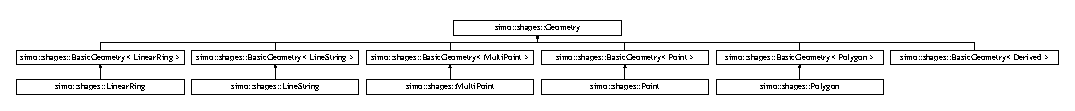
\includegraphics[height=1.048689cm]{classsimo_1_1shapes_1_1_geometry}
\end{center}
\end{figure}
\subsection*{Public Member Functions}
\begin{DoxyCompactItemize}
\item 
\hypertarget{classsimo_1_1shapes_1_1_geometry_ad0611340eaded743bbdfe0abb43c59a4}{virtual \hyperlink{classsimo_1_1shapes_1_1_geometry_ad0611340eaded743bbdfe0abb43c59a4}{$\sim$\-Geometry} ()=default}\label{classsimo_1_1shapes_1_1_geometry_ad0611340eaded743bbdfe0abb43c59a4}

\begin{DoxyCompactList}\small\item\em virtual destructor \end{DoxyCompactList}\item 
virtual Geometry\-Type \hyperlink{classsimo_1_1shapes_1_1_geometry_a97a21e31df877cd74da81e08e6e1c7ff}{type} () const =0
\begin{DoxyCompactList}\small\item\em returns the geometry type (e.\-g. Geometry\-Type\-::\-Point, Geometry\-Type\-::\-Multi\-Point) \end{DoxyCompactList}\item 
virtual Geometry\-Detailed\-Type \hyperlink{classsimo_1_1shapes_1_1_geometry_a5633ca34213554220aa19257260b2211}{detailed\-\_\-type} () const =0
\begin{DoxyCompactList}\small\item\em returns the geometry detailed type (e.\-g. Geometry\-Type\-::\-Point\-Z, Geometry\-Type\-::\-Multi\-Point\-Z\-M) \end{DoxyCompactList}\item 
virtual std\-::string \hyperlink{classsimo_1_1shapes_1_1_geometry_aa4fc3ffa8fa908f238c2917166a4f0a1}{type\-\_\-str} () const =0
\begin{DoxyCompactList}\small\item\em returns the geometry type as a string (e.\-g. \hyperlink{classsimo_1_1shapes_1_1_point}{Point}, \hyperlink{classsimo_1_1shapes_1_1_line_string}{Line\-String}) \end{DoxyCompactList}\item 
virtual bool \hyperlink{classsimo_1_1shapes_1_1_geometry_ab53733864d430504fd7ed2b564c96ef5}{empty} () const =0
\begin{DoxyCompactList}\small\item\em returns true if the geometry is empty \end{DoxyCompactList}\item 
virtual size\-\_\-t \hyperlink{classsimo_1_1shapes_1_1_geometry_a110e8a897b84c704f9009679bbbe21fc}{size} () const =0
\begin{DoxyCompactList}\small\item\em returns the geometry size \end{DoxyCompactList}\item 
virtual Dimension\-Type \hyperlink{classsimo_1_1shapes_1_1_geometry_a8db862418cec85fc52c832267449d392}{dim} () const =0
\begin{DoxyCompactList}\small\item\em returns the dimension type of the geometry \end{DoxyCompactList}\item 
virtual void \hyperlink{classsimo_1_1shapes_1_1_geometry_adbd7a14a8b4414c882cbcafa8025085d}{set\-\_\-dim} (Dimension\-Type value)=0
\begin{DoxyCompactList}\small\item\em set the dimension type \end{DoxyCompactList}\item 
virtual int8\-\_\-t \hyperlink{classsimo_1_1shapes_1_1_geometry_ab4890550ac2208165a5953a989d0b2aa}{ndim} () const =0
\begin{DoxyCompactList}\small\item\em returns the number of dimensions of the geometry \end{DoxyCompactList}\item 
virtual \hyperlink{classsimo_1_1shapes_1_1_bounds}{Bounds} \& \hyperlink{classsimo_1_1shapes_1_1_geometry_a0ed6566c6f79af7255f5950bd44f2a1e}{bounds} ()=0
\begin{DoxyCompactList}\small\item\em returns the geometry bounds \end{DoxyCompactList}\item 
virtual std\-::vector\\*
$<$ std\-::tuple$<$ double, double $>$ $>$ \hyperlink{classsimo_1_1shapes_1_1_geometry_aa45dedcadd8e44be1f9415223ca2e19d}{xy} () const =0
\begin{DoxyCompactList}\small\item\em returns the geometry (x, y) coordinates as a tuple \end{DoxyCompactList}\item 
virtual std\-::vector\\*
$<$ std\-::tuple$<$ double, double, \\*
double $>$ $>$ \hyperlink{classsimo_1_1shapes_1_1_geometry_af1a38df76e835270559acad85366f6f3}{xyz} () const =0
\begin{DoxyCompactList}\small\item\em returns the geometry (x, y, z) coordinates as a tuple \end{DoxyCompactList}\item 
virtual std\-::vector\\*
$<$ std\-::tuple$<$ double, double, \\*
double $>$ $>$ \hyperlink{classsimo_1_1shapes_1_1_geometry_aa74d24c520c7760619e17fdfd7c2eff0}{xym} () const =0
\begin{DoxyCompactList}\small\item\em returns the geometry (x, y, m) coordinates as a tuple \end{DoxyCompactList}\item 
virtual std\-::vector\\*
$<$ std\-::tuple$<$ double, double, \\*
double, double $>$ $>$ \hyperlink{classsimo_1_1shapes_1_1_geometry_a1dc27d8d1146b3057355f96d7954f979}{xyzm} () const =0
\begin{DoxyCompactList}\small\item\em returns the geometry (x, y, z, m) coordinates as a tuple \end{DoxyCompactList}\item 
virtual bool \hyperlink{classsimo_1_1shapes_1_1_geometry_a7d2d67f5845bcccca7d88619b0be288a}{has\-\_\-z} () const =0
\begin{DoxyCompactList}\small\item\em whether the geometry has z-\/coordinate \end{DoxyCompactList}\item 
virtual bool \hyperlink{classsimo_1_1shapes_1_1_geometry_aa6b0b9e19c782d137effc7be2e5416a1}{has\-\_\-m} () const =0
\begin{DoxyCompactList}\small\item\em whether the geometry has m-\/coordinate \end{DoxyCompactList}\item 
virtual bool \hyperlink{classsimo_1_1shapes_1_1_geometry_a2c1ea77c6f3b7b6c20eb9894be264f80}{is\-\_\-closed} () const =0
\begin{DoxyCompactList}\small\item\em whether the geometry is closed \end{DoxyCompactList}\end{DoxyCompactItemize}


\subsection{Detailed Description}
geometry interface 

Definition at line 15 of file geometry.\-hpp.



\subsection{Member Function Documentation}
\hypertarget{classsimo_1_1shapes_1_1_geometry_a0ed6566c6f79af7255f5950bd44f2a1e}{\index{simo\-::shapes\-::\-Geometry@{simo\-::shapes\-::\-Geometry}!bounds@{bounds}}
\index{bounds@{bounds}!simo::shapes::Geometry@{simo\-::shapes\-::\-Geometry}}
\subsubsection[{bounds}]{\setlength{\rightskip}{0pt plus 5cm}virtual {\bf Bounds}\& simo\-::shapes\-::\-Geometry\-::bounds (
\begin{DoxyParamCaption}
{}
\end{DoxyParamCaption}
)\hspace{0.3cm}{\ttfamily [pure virtual]}}}\label{classsimo_1_1shapes_1_1_geometry_a0ed6566c6f79af7255f5950bd44f2a1e}


returns the geometry bounds 

\begin{DoxyReturn}{Returns}
the geometry bounds
\end{DoxyReturn}
\begin{DoxySince}{Since}
0.\-0.\-1 
\end{DoxySince}


Implemented in \hyperlink{classsimo_1_1shapes_1_1_basic_geometry_aef057b58858f64a47a8fa68b7a9ef7d1}{simo\-::shapes\-::\-Basic\-Geometry$<$ Derived $>$}, \hyperlink{classsimo_1_1shapes_1_1_basic_geometry_aef057b58858f64a47a8fa68b7a9ef7d1}{simo\-::shapes\-::\-Basic\-Geometry$<$ Linear\-Ring $>$}, \hyperlink{classsimo_1_1shapes_1_1_basic_geometry_aef057b58858f64a47a8fa68b7a9ef7d1}{simo\-::shapes\-::\-Basic\-Geometry$<$ Line\-String $>$}, \hyperlink{classsimo_1_1shapes_1_1_basic_geometry_aef057b58858f64a47a8fa68b7a9ef7d1}{simo\-::shapes\-::\-Basic\-Geometry$<$ Polygon $>$}, \hyperlink{classsimo_1_1shapes_1_1_basic_geometry_aef057b58858f64a47a8fa68b7a9ef7d1}{simo\-::shapes\-::\-Basic\-Geometry$<$ Multi\-Point $>$}, and \hyperlink{classsimo_1_1shapes_1_1_basic_geometry_aef057b58858f64a47a8fa68b7a9ef7d1}{simo\-::shapes\-::\-Basic\-Geometry$<$ Point $>$}.

\hypertarget{classsimo_1_1shapes_1_1_geometry_a5633ca34213554220aa19257260b2211}{\index{simo\-::shapes\-::\-Geometry@{simo\-::shapes\-::\-Geometry}!detailed\-\_\-type@{detailed\-\_\-type}}
\index{detailed\-\_\-type@{detailed\-\_\-type}!simo::shapes::Geometry@{simo\-::shapes\-::\-Geometry}}
\subsubsection[{detailed\-\_\-type}]{\setlength{\rightskip}{0pt plus 5cm}virtual Geometry\-Detailed\-Type simo\-::shapes\-::\-Geometry\-::detailed\-\_\-type (
\begin{DoxyParamCaption}
{}
\end{DoxyParamCaption}
) const\hspace{0.3cm}{\ttfamily [pure virtual]}}}\label{classsimo_1_1shapes_1_1_geometry_a5633ca34213554220aa19257260b2211}


returns the geometry detailed type (e.\-g. Geometry\-Type\-::\-Point\-Z, Geometry\-Type\-::\-Multi\-Point\-Z\-M) 

\begin{DoxyReturn}{Returns}
the geometry detailed type
\end{DoxyReturn}
\begin{DoxySince}{Since}
0.\-0.\-1 
\end{DoxySince}


Implemented in \hyperlink{classsimo_1_1shapes_1_1_basic_geometry_a82ea146df5c632a15864fc56817d6d0f}{simo\-::shapes\-::\-Basic\-Geometry$<$ Derived $>$}, \hyperlink{classsimo_1_1shapes_1_1_basic_geometry_a82ea146df5c632a15864fc56817d6d0f}{simo\-::shapes\-::\-Basic\-Geometry$<$ Linear\-Ring $>$}, \hyperlink{classsimo_1_1shapes_1_1_basic_geometry_a82ea146df5c632a15864fc56817d6d0f}{simo\-::shapes\-::\-Basic\-Geometry$<$ Line\-String $>$}, \hyperlink{classsimo_1_1shapes_1_1_basic_geometry_a82ea146df5c632a15864fc56817d6d0f}{simo\-::shapes\-::\-Basic\-Geometry$<$ Polygon $>$}, \hyperlink{classsimo_1_1shapes_1_1_basic_geometry_a82ea146df5c632a15864fc56817d6d0f}{simo\-::shapes\-::\-Basic\-Geometry$<$ Multi\-Point $>$}, and \hyperlink{classsimo_1_1shapes_1_1_basic_geometry_a82ea146df5c632a15864fc56817d6d0f}{simo\-::shapes\-::\-Basic\-Geometry$<$ Point $>$}.

\hypertarget{classsimo_1_1shapes_1_1_geometry_a8db862418cec85fc52c832267449d392}{\index{simo\-::shapes\-::\-Geometry@{simo\-::shapes\-::\-Geometry}!dim@{dim}}
\index{dim@{dim}!simo::shapes::Geometry@{simo\-::shapes\-::\-Geometry}}
\subsubsection[{dim}]{\setlength{\rightskip}{0pt plus 5cm}virtual Dimension\-Type simo\-::shapes\-::\-Geometry\-::dim (
\begin{DoxyParamCaption}
{}
\end{DoxyParamCaption}
) const\hspace{0.3cm}{\ttfamily [pure virtual]}}}\label{classsimo_1_1shapes_1_1_geometry_a8db862418cec85fc52c832267449d392}


returns the dimension type of the geometry 

\begin{DoxyReturn}{Returns}
the dimension type
\end{DoxyReturn}
\begin{DoxyNote}{Note}
the dimension type is (x, y), (x, y, z), (x, y, m) and (x, y, z, m)
\end{DoxyNote}
\begin{DoxySince}{Since}
0.\-0.\-1 
\end{DoxySince}


Implemented in \hyperlink{classsimo_1_1shapes_1_1_basic_geometry_aa2cf098bf849207e3c1a638a31d28685}{simo\-::shapes\-::\-Basic\-Geometry$<$ Derived $>$}, \hyperlink{classsimo_1_1shapes_1_1_basic_geometry_aa2cf098bf849207e3c1a638a31d28685}{simo\-::shapes\-::\-Basic\-Geometry$<$ Linear\-Ring $>$}, \hyperlink{classsimo_1_1shapes_1_1_basic_geometry_aa2cf098bf849207e3c1a638a31d28685}{simo\-::shapes\-::\-Basic\-Geometry$<$ Line\-String $>$}, \hyperlink{classsimo_1_1shapes_1_1_basic_geometry_aa2cf098bf849207e3c1a638a31d28685}{simo\-::shapes\-::\-Basic\-Geometry$<$ Polygon $>$}, \hyperlink{classsimo_1_1shapes_1_1_basic_geometry_aa2cf098bf849207e3c1a638a31d28685}{simo\-::shapes\-::\-Basic\-Geometry$<$ Multi\-Point $>$}, and \hyperlink{classsimo_1_1shapes_1_1_basic_geometry_aa2cf098bf849207e3c1a638a31d28685}{simo\-::shapes\-::\-Basic\-Geometry$<$ Point $>$}.

\hypertarget{classsimo_1_1shapes_1_1_geometry_ab53733864d430504fd7ed2b564c96ef5}{\index{simo\-::shapes\-::\-Geometry@{simo\-::shapes\-::\-Geometry}!empty@{empty}}
\index{empty@{empty}!simo::shapes::Geometry@{simo\-::shapes\-::\-Geometry}}
\subsubsection[{empty}]{\setlength{\rightskip}{0pt plus 5cm}virtual bool simo\-::shapes\-::\-Geometry\-::empty (
\begin{DoxyParamCaption}
{}
\end{DoxyParamCaption}
) const\hspace{0.3cm}{\ttfamily [pure virtual]}}}\label{classsimo_1_1shapes_1_1_geometry_ab53733864d430504fd7ed2b564c96ef5}


returns true if the geometry is empty 

\begin{DoxyReturn}{Returns}
true if the the geometry is empty, otherwise false
\end{DoxyReturn}
\begin{DoxySince}{Since}
0.\-0.\-1 
\end{DoxySince}


Implemented in \hyperlink{classsimo_1_1shapes_1_1_basic_geometry_a6834cf02c916d416b84d66d03fa7a525}{simo\-::shapes\-::\-Basic\-Geometry$<$ Derived $>$}, \hyperlink{classsimo_1_1shapes_1_1_basic_geometry_a6834cf02c916d416b84d66d03fa7a525}{simo\-::shapes\-::\-Basic\-Geometry$<$ Linear\-Ring $>$}, \hyperlink{classsimo_1_1shapes_1_1_basic_geometry_a6834cf02c916d416b84d66d03fa7a525}{simo\-::shapes\-::\-Basic\-Geometry$<$ Line\-String $>$}, \hyperlink{classsimo_1_1shapes_1_1_basic_geometry_a6834cf02c916d416b84d66d03fa7a525}{simo\-::shapes\-::\-Basic\-Geometry$<$ Polygon $>$}, \hyperlink{classsimo_1_1shapes_1_1_basic_geometry_a6834cf02c916d416b84d66d03fa7a525}{simo\-::shapes\-::\-Basic\-Geometry$<$ Multi\-Point $>$}, and \hyperlink{classsimo_1_1shapes_1_1_basic_geometry_a6834cf02c916d416b84d66d03fa7a525}{simo\-::shapes\-::\-Basic\-Geometry$<$ Point $>$}.

\hypertarget{classsimo_1_1shapes_1_1_geometry_aa6b0b9e19c782d137effc7be2e5416a1}{\index{simo\-::shapes\-::\-Geometry@{simo\-::shapes\-::\-Geometry}!has\-\_\-m@{has\-\_\-m}}
\index{has\-\_\-m@{has\-\_\-m}!simo::shapes::Geometry@{simo\-::shapes\-::\-Geometry}}
\subsubsection[{has\-\_\-m}]{\setlength{\rightskip}{0pt plus 5cm}virtual bool simo\-::shapes\-::\-Geometry\-::has\-\_\-m (
\begin{DoxyParamCaption}
{}
\end{DoxyParamCaption}
) const\hspace{0.3cm}{\ttfamily [pure virtual]}}}\label{classsimo_1_1shapes_1_1_geometry_aa6b0b9e19c782d137effc7be2e5416a1}


whether the geometry has m-\/coordinate 

\begin{DoxyReturn}{Returns}
true if the geometry has m-\/coordinate, otherwise false
\end{DoxyReturn}
\begin{DoxySince}{Since}
0.\-0.\-1 
\end{DoxySince}


Implemented in \hyperlink{classsimo_1_1shapes_1_1_basic_geometry_ae67e31810708aa668749f1d1ae8ae28b}{simo\-::shapes\-::\-Basic\-Geometry$<$ Derived $>$}, \hyperlink{classsimo_1_1shapes_1_1_basic_geometry_ae67e31810708aa668749f1d1ae8ae28b}{simo\-::shapes\-::\-Basic\-Geometry$<$ Linear\-Ring $>$}, \hyperlink{classsimo_1_1shapes_1_1_basic_geometry_ae67e31810708aa668749f1d1ae8ae28b}{simo\-::shapes\-::\-Basic\-Geometry$<$ Line\-String $>$}, \hyperlink{classsimo_1_1shapes_1_1_basic_geometry_ae67e31810708aa668749f1d1ae8ae28b}{simo\-::shapes\-::\-Basic\-Geometry$<$ Polygon $>$}, \hyperlink{classsimo_1_1shapes_1_1_basic_geometry_ae67e31810708aa668749f1d1ae8ae28b}{simo\-::shapes\-::\-Basic\-Geometry$<$ Multi\-Point $>$}, and \hyperlink{classsimo_1_1shapes_1_1_basic_geometry_ae67e31810708aa668749f1d1ae8ae28b}{simo\-::shapes\-::\-Basic\-Geometry$<$ Point $>$}.

\hypertarget{classsimo_1_1shapes_1_1_geometry_a7d2d67f5845bcccca7d88619b0be288a}{\index{simo\-::shapes\-::\-Geometry@{simo\-::shapes\-::\-Geometry}!has\-\_\-z@{has\-\_\-z}}
\index{has\-\_\-z@{has\-\_\-z}!simo::shapes::Geometry@{simo\-::shapes\-::\-Geometry}}
\subsubsection[{has\-\_\-z}]{\setlength{\rightskip}{0pt plus 5cm}virtual bool simo\-::shapes\-::\-Geometry\-::has\-\_\-z (
\begin{DoxyParamCaption}
{}
\end{DoxyParamCaption}
) const\hspace{0.3cm}{\ttfamily [pure virtual]}}}\label{classsimo_1_1shapes_1_1_geometry_a7d2d67f5845bcccca7d88619b0be288a}


whether the geometry has z-\/coordinate 

\begin{DoxyReturn}{Returns}
true if the geometry has z-\/coordinate, otherwise false
\end{DoxyReturn}
\begin{DoxySince}{Since}
0.\-0.\-1 
\end{DoxySince}


Implemented in \hyperlink{classsimo_1_1shapes_1_1_basic_geometry_adf922693df08f41d170438836bc90c6b}{simo\-::shapes\-::\-Basic\-Geometry$<$ Derived $>$}, \hyperlink{classsimo_1_1shapes_1_1_basic_geometry_adf922693df08f41d170438836bc90c6b}{simo\-::shapes\-::\-Basic\-Geometry$<$ Linear\-Ring $>$}, \hyperlink{classsimo_1_1shapes_1_1_basic_geometry_adf922693df08f41d170438836bc90c6b}{simo\-::shapes\-::\-Basic\-Geometry$<$ Line\-String $>$}, \hyperlink{classsimo_1_1shapes_1_1_basic_geometry_adf922693df08f41d170438836bc90c6b}{simo\-::shapes\-::\-Basic\-Geometry$<$ Polygon $>$}, \hyperlink{classsimo_1_1shapes_1_1_basic_geometry_adf922693df08f41d170438836bc90c6b}{simo\-::shapes\-::\-Basic\-Geometry$<$ Multi\-Point $>$}, and \hyperlink{classsimo_1_1shapes_1_1_basic_geometry_adf922693df08f41d170438836bc90c6b}{simo\-::shapes\-::\-Basic\-Geometry$<$ Point $>$}.

\hypertarget{classsimo_1_1shapes_1_1_geometry_a2c1ea77c6f3b7b6c20eb9894be264f80}{\index{simo\-::shapes\-::\-Geometry@{simo\-::shapes\-::\-Geometry}!is\-\_\-closed@{is\-\_\-closed}}
\index{is\-\_\-closed@{is\-\_\-closed}!simo::shapes::Geometry@{simo\-::shapes\-::\-Geometry}}
\subsubsection[{is\-\_\-closed}]{\setlength{\rightskip}{0pt plus 5cm}virtual bool simo\-::shapes\-::\-Geometry\-::is\-\_\-closed (
\begin{DoxyParamCaption}
{}
\end{DoxyParamCaption}
) const\hspace{0.3cm}{\ttfamily [pure virtual]}}}\label{classsimo_1_1shapes_1_1_geometry_a2c1ea77c6f3b7b6c20eb9894be264f80}


whether the geometry is closed 

\begin{DoxyReturn}{Returns}
true if the geometry is closed, otherwise false
\end{DoxyReturn}
\begin{DoxySince}{Since}
0.\-0.\-1 
\end{DoxySince}


Implemented in \hyperlink{classsimo_1_1shapes_1_1_basic_geometry_ae5ad57479626834ef3c4e10c2fb2275b}{simo\-::shapes\-::\-Basic\-Geometry$<$ Derived $>$}, \hyperlink{classsimo_1_1shapes_1_1_basic_geometry_ae5ad57479626834ef3c4e10c2fb2275b}{simo\-::shapes\-::\-Basic\-Geometry$<$ Linear\-Ring $>$}, \hyperlink{classsimo_1_1shapes_1_1_basic_geometry_ae5ad57479626834ef3c4e10c2fb2275b}{simo\-::shapes\-::\-Basic\-Geometry$<$ Line\-String $>$}, \hyperlink{classsimo_1_1shapes_1_1_basic_geometry_ae5ad57479626834ef3c4e10c2fb2275b}{simo\-::shapes\-::\-Basic\-Geometry$<$ Polygon $>$}, \hyperlink{classsimo_1_1shapes_1_1_basic_geometry_ae5ad57479626834ef3c4e10c2fb2275b}{simo\-::shapes\-::\-Basic\-Geometry$<$ Multi\-Point $>$}, and \hyperlink{classsimo_1_1shapes_1_1_basic_geometry_ae5ad57479626834ef3c4e10c2fb2275b}{simo\-::shapes\-::\-Basic\-Geometry$<$ Point $>$}.

\hypertarget{classsimo_1_1shapes_1_1_geometry_ab4890550ac2208165a5953a989d0b2aa}{\index{simo\-::shapes\-::\-Geometry@{simo\-::shapes\-::\-Geometry}!ndim@{ndim}}
\index{ndim@{ndim}!simo::shapes::Geometry@{simo\-::shapes\-::\-Geometry}}
\subsubsection[{ndim}]{\setlength{\rightskip}{0pt plus 5cm}virtual int8\-\_\-t simo\-::shapes\-::\-Geometry\-::ndim (
\begin{DoxyParamCaption}
{}
\end{DoxyParamCaption}
) const\hspace{0.3cm}{\ttfamily [pure virtual]}}}\label{classsimo_1_1shapes_1_1_geometry_ab4890550ac2208165a5953a989d0b2aa}


returns the number of dimensions of the geometry 

\begin{DoxyReturn}{Returns}
the number of dimensions
\end{DoxyReturn}
\begin{DoxyNote}{Note}
the number of dimensions is (x, y) = 2, (x, y, z) = 3, (x, y, m) = 3 and (x, y, z, m) = 4
\end{DoxyNote}
\begin{DoxySince}{Since}
0.\-0.\-1 
\end{DoxySince}


Implemented in \hyperlink{classsimo_1_1shapes_1_1_basic_geometry_ae5ae8173a8c166d98ddda0fbfbc48346}{simo\-::shapes\-::\-Basic\-Geometry$<$ Derived $>$}, \hyperlink{classsimo_1_1shapes_1_1_basic_geometry_ae5ae8173a8c166d98ddda0fbfbc48346}{simo\-::shapes\-::\-Basic\-Geometry$<$ Linear\-Ring $>$}, \hyperlink{classsimo_1_1shapes_1_1_basic_geometry_ae5ae8173a8c166d98ddda0fbfbc48346}{simo\-::shapes\-::\-Basic\-Geometry$<$ Line\-String $>$}, \hyperlink{classsimo_1_1shapes_1_1_basic_geometry_ae5ae8173a8c166d98ddda0fbfbc48346}{simo\-::shapes\-::\-Basic\-Geometry$<$ Polygon $>$}, \hyperlink{classsimo_1_1shapes_1_1_basic_geometry_ae5ae8173a8c166d98ddda0fbfbc48346}{simo\-::shapes\-::\-Basic\-Geometry$<$ Multi\-Point $>$}, and \hyperlink{classsimo_1_1shapes_1_1_basic_geometry_ae5ae8173a8c166d98ddda0fbfbc48346}{simo\-::shapes\-::\-Basic\-Geometry$<$ Point $>$}.

\hypertarget{classsimo_1_1shapes_1_1_geometry_adbd7a14a8b4414c882cbcafa8025085d}{\index{simo\-::shapes\-::\-Geometry@{simo\-::shapes\-::\-Geometry}!set\-\_\-dim@{set\-\_\-dim}}
\index{set\-\_\-dim@{set\-\_\-dim}!simo::shapes::Geometry@{simo\-::shapes\-::\-Geometry}}
\subsubsection[{set\-\_\-dim}]{\setlength{\rightskip}{0pt plus 5cm}virtual void simo\-::shapes\-::\-Geometry\-::set\-\_\-dim (
\begin{DoxyParamCaption}
\item[{Dimension\-Type}]{value}
\end{DoxyParamCaption}
)\hspace{0.3cm}{\ttfamily [pure virtual]}}}\label{classsimo_1_1shapes_1_1_geometry_adbd7a14a8b4414c882cbcafa8025085d}


set the dimension type 


\begin{DoxyParams}{Parameters}
{\em value} & the dimension type\\
\hline
\end{DoxyParams}
\begin{DoxySince}{Since}
0.\-0.\-1 
\end{DoxySince}


Implemented in \hyperlink{classsimo_1_1shapes_1_1_basic_geometry_a203dc3ca9965a82151ec17299a429730}{simo\-::shapes\-::\-Basic\-Geometry$<$ Derived $>$}, \hyperlink{classsimo_1_1shapes_1_1_basic_geometry_a203dc3ca9965a82151ec17299a429730}{simo\-::shapes\-::\-Basic\-Geometry$<$ Linear\-Ring $>$}, \hyperlink{classsimo_1_1shapes_1_1_basic_geometry_a203dc3ca9965a82151ec17299a429730}{simo\-::shapes\-::\-Basic\-Geometry$<$ Line\-String $>$}, \hyperlink{classsimo_1_1shapes_1_1_basic_geometry_a203dc3ca9965a82151ec17299a429730}{simo\-::shapes\-::\-Basic\-Geometry$<$ Polygon $>$}, \hyperlink{classsimo_1_1shapes_1_1_basic_geometry_a203dc3ca9965a82151ec17299a429730}{simo\-::shapes\-::\-Basic\-Geometry$<$ Multi\-Point $>$}, and \hyperlink{classsimo_1_1shapes_1_1_basic_geometry_a203dc3ca9965a82151ec17299a429730}{simo\-::shapes\-::\-Basic\-Geometry$<$ Point $>$}.

\hypertarget{classsimo_1_1shapes_1_1_geometry_a110e8a897b84c704f9009679bbbe21fc}{\index{simo\-::shapes\-::\-Geometry@{simo\-::shapes\-::\-Geometry}!size@{size}}
\index{size@{size}!simo::shapes::Geometry@{simo\-::shapes\-::\-Geometry}}
\subsubsection[{size}]{\setlength{\rightskip}{0pt plus 5cm}virtual size\-\_\-t simo\-::shapes\-::\-Geometry\-::size (
\begin{DoxyParamCaption}
{}
\end{DoxyParamCaption}
) const\hspace{0.3cm}{\ttfamily [pure virtual]}}}\label{classsimo_1_1shapes_1_1_geometry_a110e8a897b84c704f9009679bbbe21fc}


returns the geometry size 

\begin{DoxyReturn}{Returns}
the size of the geometry
\end{DoxyReturn}
\begin{DoxySince}{Since}
0.\-0.\-1 
\end{DoxySince}


Implemented in \hyperlink{classsimo_1_1shapes_1_1_basic_geometry_a5e68b783fac81ad8e6c38a0c86875423}{simo\-::shapes\-::\-Basic\-Geometry$<$ Derived $>$}, \hyperlink{classsimo_1_1shapes_1_1_basic_geometry_a5e68b783fac81ad8e6c38a0c86875423}{simo\-::shapes\-::\-Basic\-Geometry$<$ Linear\-Ring $>$}, \hyperlink{classsimo_1_1shapes_1_1_basic_geometry_a5e68b783fac81ad8e6c38a0c86875423}{simo\-::shapes\-::\-Basic\-Geometry$<$ Line\-String $>$}, \hyperlink{classsimo_1_1shapes_1_1_basic_geometry_a5e68b783fac81ad8e6c38a0c86875423}{simo\-::shapes\-::\-Basic\-Geometry$<$ Polygon $>$}, \hyperlink{classsimo_1_1shapes_1_1_basic_geometry_a5e68b783fac81ad8e6c38a0c86875423}{simo\-::shapes\-::\-Basic\-Geometry$<$ Multi\-Point $>$}, and \hyperlink{classsimo_1_1shapes_1_1_basic_geometry_a5e68b783fac81ad8e6c38a0c86875423}{simo\-::shapes\-::\-Basic\-Geometry$<$ Point $>$}.

\hypertarget{classsimo_1_1shapes_1_1_geometry_a97a21e31df877cd74da81e08e6e1c7ff}{\index{simo\-::shapes\-::\-Geometry@{simo\-::shapes\-::\-Geometry}!type@{type}}
\index{type@{type}!simo::shapes::Geometry@{simo\-::shapes\-::\-Geometry}}
\subsubsection[{type}]{\setlength{\rightskip}{0pt plus 5cm}virtual Geometry\-Type simo\-::shapes\-::\-Geometry\-::type (
\begin{DoxyParamCaption}
{}
\end{DoxyParamCaption}
) const\hspace{0.3cm}{\ttfamily [pure virtual]}}}\label{classsimo_1_1shapes_1_1_geometry_a97a21e31df877cd74da81e08e6e1c7ff}


returns the geometry type (e.\-g. Geometry\-Type\-::\-Point, Geometry\-Type\-::\-Multi\-Point) 

\begin{DoxyReturn}{Returns}
the geometry type
\end{DoxyReturn}
\begin{DoxySince}{Since}
0.\-0.\-1 
\end{DoxySince}


Implemented in \hyperlink{classsimo_1_1shapes_1_1_basic_geometry_a8cb2eba04f6fb0cb80cd9c9d2c85f213}{simo\-::shapes\-::\-Basic\-Geometry$<$ Derived $>$}, \hyperlink{classsimo_1_1shapes_1_1_basic_geometry_a8cb2eba04f6fb0cb80cd9c9d2c85f213}{simo\-::shapes\-::\-Basic\-Geometry$<$ Linear\-Ring $>$}, \hyperlink{classsimo_1_1shapes_1_1_basic_geometry_a8cb2eba04f6fb0cb80cd9c9d2c85f213}{simo\-::shapes\-::\-Basic\-Geometry$<$ Line\-String $>$}, \hyperlink{classsimo_1_1shapes_1_1_basic_geometry_a8cb2eba04f6fb0cb80cd9c9d2c85f213}{simo\-::shapes\-::\-Basic\-Geometry$<$ Polygon $>$}, \hyperlink{classsimo_1_1shapes_1_1_basic_geometry_a8cb2eba04f6fb0cb80cd9c9d2c85f213}{simo\-::shapes\-::\-Basic\-Geometry$<$ Multi\-Point $>$}, and \hyperlink{classsimo_1_1shapes_1_1_basic_geometry_a8cb2eba04f6fb0cb80cd9c9d2c85f213}{simo\-::shapes\-::\-Basic\-Geometry$<$ Point $>$}.

\hypertarget{classsimo_1_1shapes_1_1_geometry_aa4fc3ffa8fa908f238c2917166a4f0a1}{\index{simo\-::shapes\-::\-Geometry@{simo\-::shapes\-::\-Geometry}!type\-\_\-str@{type\-\_\-str}}
\index{type\-\_\-str@{type\-\_\-str}!simo::shapes::Geometry@{simo\-::shapes\-::\-Geometry}}
\subsubsection[{type\-\_\-str}]{\setlength{\rightskip}{0pt plus 5cm}virtual std\-::string simo\-::shapes\-::\-Geometry\-::type\-\_\-str (
\begin{DoxyParamCaption}
{}
\end{DoxyParamCaption}
) const\hspace{0.3cm}{\ttfamily [pure virtual]}}}\label{classsimo_1_1shapes_1_1_geometry_aa4fc3ffa8fa908f238c2917166a4f0a1}


returns the geometry type as a string (e.\-g. \hyperlink{classsimo_1_1shapes_1_1_point}{Point}, \hyperlink{classsimo_1_1shapes_1_1_line_string}{Line\-String}) 

\begin{DoxyReturn}{Returns}
the geometry type as a string
\end{DoxyReturn}
\begin{DoxySince}{Since}
0.\-0.\-1 
\end{DoxySince}


Implemented in \hyperlink{classsimo_1_1shapes_1_1_basic_geometry_ad2331ba481d41c9f7089787a32ef4ced}{simo\-::shapes\-::\-Basic\-Geometry$<$ Derived $>$}, \hyperlink{classsimo_1_1shapes_1_1_basic_geometry_ad2331ba481d41c9f7089787a32ef4ced}{simo\-::shapes\-::\-Basic\-Geometry$<$ Linear\-Ring $>$}, \hyperlink{classsimo_1_1shapes_1_1_basic_geometry_ad2331ba481d41c9f7089787a32ef4ced}{simo\-::shapes\-::\-Basic\-Geometry$<$ Line\-String $>$}, \hyperlink{classsimo_1_1shapes_1_1_basic_geometry_ad2331ba481d41c9f7089787a32ef4ced}{simo\-::shapes\-::\-Basic\-Geometry$<$ Polygon $>$}, \hyperlink{classsimo_1_1shapes_1_1_basic_geometry_ad2331ba481d41c9f7089787a32ef4ced}{simo\-::shapes\-::\-Basic\-Geometry$<$ Multi\-Point $>$}, and \hyperlink{classsimo_1_1shapes_1_1_basic_geometry_ad2331ba481d41c9f7089787a32ef4ced}{simo\-::shapes\-::\-Basic\-Geometry$<$ Point $>$}.

\hypertarget{classsimo_1_1shapes_1_1_geometry_aa45dedcadd8e44be1f9415223ca2e19d}{\index{simo\-::shapes\-::\-Geometry@{simo\-::shapes\-::\-Geometry}!xy@{xy}}
\index{xy@{xy}!simo::shapes::Geometry@{simo\-::shapes\-::\-Geometry}}
\subsubsection[{xy}]{\setlength{\rightskip}{0pt plus 5cm}virtual std\-::vector$<$std\-::tuple$<$double, double$>$ $>$ simo\-::shapes\-::\-Geometry\-::xy (
\begin{DoxyParamCaption}
{}
\end{DoxyParamCaption}
) const\hspace{0.3cm}{\ttfamily [pure virtual]}}}\label{classsimo_1_1shapes_1_1_geometry_aa45dedcadd8e44be1f9415223ca2e19d}


returns the geometry (x, y) coordinates as a tuple 

\begin{DoxyReturn}{Returns}
a vector of (x, y) tuples
\end{DoxyReturn}
\begin{DoxySince}{Since}
0.\-0.\-1 
\end{DoxySince}


Implemented in \hyperlink{classsimo_1_1shapes_1_1_basic_geometry_a492b93c475d7a059b4be04a2aafddc99}{simo\-::shapes\-::\-Basic\-Geometry$<$ Derived $>$}, \hyperlink{classsimo_1_1shapes_1_1_basic_geometry_a492b93c475d7a059b4be04a2aafddc99}{simo\-::shapes\-::\-Basic\-Geometry$<$ Linear\-Ring $>$}, \hyperlink{classsimo_1_1shapes_1_1_basic_geometry_a492b93c475d7a059b4be04a2aafddc99}{simo\-::shapes\-::\-Basic\-Geometry$<$ Line\-String $>$}, \hyperlink{classsimo_1_1shapes_1_1_basic_geometry_a492b93c475d7a059b4be04a2aafddc99}{simo\-::shapes\-::\-Basic\-Geometry$<$ Polygon $>$}, \hyperlink{classsimo_1_1shapes_1_1_basic_geometry_a492b93c475d7a059b4be04a2aafddc99}{simo\-::shapes\-::\-Basic\-Geometry$<$ Multi\-Point $>$}, and \hyperlink{classsimo_1_1shapes_1_1_basic_geometry_a492b93c475d7a059b4be04a2aafddc99}{simo\-::shapes\-::\-Basic\-Geometry$<$ Point $>$}.

\hypertarget{classsimo_1_1shapes_1_1_geometry_aa74d24c520c7760619e17fdfd7c2eff0}{\index{simo\-::shapes\-::\-Geometry@{simo\-::shapes\-::\-Geometry}!xym@{xym}}
\index{xym@{xym}!simo::shapes::Geometry@{simo\-::shapes\-::\-Geometry}}
\subsubsection[{xym}]{\setlength{\rightskip}{0pt plus 5cm}virtual std\-::vector$<$std\-::tuple$<$double, double, double$>$ $>$ simo\-::shapes\-::\-Geometry\-::xym (
\begin{DoxyParamCaption}
{}
\end{DoxyParamCaption}
) const\hspace{0.3cm}{\ttfamily [pure virtual]}}}\label{classsimo_1_1shapes_1_1_geometry_aa74d24c520c7760619e17fdfd7c2eff0}


returns the geometry (x, y, m) coordinates as a tuple 

\begin{DoxyReturn}{Returns}
a vector of (x, y, m) tuples
\end{DoxyReturn}
\begin{DoxySince}{Since}
0.\-0.\-1 
\end{DoxySince}


Implemented in \hyperlink{classsimo_1_1shapes_1_1_basic_geometry_ad6f72ade4686897fbea8f3b616b06df8}{simo\-::shapes\-::\-Basic\-Geometry$<$ Derived $>$}, \hyperlink{classsimo_1_1shapes_1_1_basic_geometry_ad6f72ade4686897fbea8f3b616b06df8}{simo\-::shapes\-::\-Basic\-Geometry$<$ Linear\-Ring $>$}, \hyperlink{classsimo_1_1shapes_1_1_basic_geometry_ad6f72ade4686897fbea8f3b616b06df8}{simo\-::shapes\-::\-Basic\-Geometry$<$ Line\-String $>$}, \hyperlink{classsimo_1_1shapes_1_1_basic_geometry_ad6f72ade4686897fbea8f3b616b06df8}{simo\-::shapes\-::\-Basic\-Geometry$<$ Polygon $>$}, \hyperlink{classsimo_1_1shapes_1_1_basic_geometry_ad6f72ade4686897fbea8f3b616b06df8}{simo\-::shapes\-::\-Basic\-Geometry$<$ Multi\-Point $>$}, and \hyperlink{classsimo_1_1shapes_1_1_basic_geometry_ad6f72ade4686897fbea8f3b616b06df8}{simo\-::shapes\-::\-Basic\-Geometry$<$ Point $>$}.

\hypertarget{classsimo_1_1shapes_1_1_geometry_af1a38df76e835270559acad85366f6f3}{\index{simo\-::shapes\-::\-Geometry@{simo\-::shapes\-::\-Geometry}!xyz@{xyz}}
\index{xyz@{xyz}!simo::shapes::Geometry@{simo\-::shapes\-::\-Geometry}}
\subsubsection[{xyz}]{\setlength{\rightskip}{0pt plus 5cm}virtual std\-::vector$<$std\-::tuple$<$double, double, double$>$ $>$ simo\-::shapes\-::\-Geometry\-::xyz (
\begin{DoxyParamCaption}
{}
\end{DoxyParamCaption}
) const\hspace{0.3cm}{\ttfamily [pure virtual]}}}\label{classsimo_1_1shapes_1_1_geometry_af1a38df76e835270559acad85366f6f3}


returns the geometry (x, y, z) coordinates as a tuple 

\begin{DoxyReturn}{Returns}
a vector of (x, y, z) tuples
\end{DoxyReturn}
\begin{DoxySince}{Since}
0.\-0.\-1 
\end{DoxySince}


Implemented in \hyperlink{classsimo_1_1shapes_1_1_basic_geometry_ad0098dca3aab7d3f710d21b672935570}{simo\-::shapes\-::\-Basic\-Geometry$<$ Derived $>$}, \hyperlink{classsimo_1_1shapes_1_1_basic_geometry_ad0098dca3aab7d3f710d21b672935570}{simo\-::shapes\-::\-Basic\-Geometry$<$ Linear\-Ring $>$}, \hyperlink{classsimo_1_1shapes_1_1_basic_geometry_ad0098dca3aab7d3f710d21b672935570}{simo\-::shapes\-::\-Basic\-Geometry$<$ Line\-String $>$}, \hyperlink{classsimo_1_1shapes_1_1_basic_geometry_ad0098dca3aab7d3f710d21b672935570}{simo\-::shapes\-::\-Basic\-Geometry$<$ Polygon $>$}, \hyperlink{classsimo_1_1shapes_1_1_basic_geometry_ad0098dca3aab7d3f710d21b672935570}{simo\-::shapes\-::\-Basic\-Geometry$<$ Multi\-Point $>$}, and \hyperlink{classsimo_1_1shapes_1_1_basic_geometry_ad0098dca3aab7d3f710d21b672935570}{simo\-::shapes\-::\-Basic\-Geometry$<$ Point $>$}.

\hypertarget{classsimo_1_1shapes_1_1_geometry_a1dc27d8d1146b3057355f96d7954f979}{\index{simo\-::shapes\-::\-Geometry@{simo\-::shapes\-::\-Geometry}!xyzm@{xyzm}}
\index{xyzm@{xyzm}!simo::shapes::Geometry@{simo\-::shapes\-::\-Geometry}}
\subsubsection[{xyzm}]{\setlength{\rightskip}{0pt plus 5cm}virtual std\-::vector$<$std\-::tuple$<$double, double, double, double$>$ $>$ simo\-::shapes\-::\-Geometry\-::xyzm (
\begin{DoxyParamCaption}
{}
\end{DoxyParamCaption}
) const\hspace{0.3cm}{\ttfamily [pure virtual]}}}\label{classsimo_1_1shapes_1_1_geometry_a1dc27d8d1146b3057355f96d7954f979}


returns the geometry (x, y, z, m) coordinates as a tuple 

\begin{DoxyReturn}{Returns}
a vector of (x, y, z, m) tuples
\end{DoxyReturn}
\begin{DoxySince}{Since}
0.\-0.\-1 
\end{DoxySince}


Implemented in \hyperlink{classsimo_1_1shapes_1_1_basic_geometry_a94dd1ee38d7b46ce92d1f547293fedce}{simo\-::shapes\-::\-Basic\-Geometry$<$ Derived $>$}, \hyperlink{classsimo_1_1shapes_1_1_basic_geometry_a94dd1ee38d7b46ce92d1f547293fedce}{simo\-::shapes\-::\-Basic\-Geometry$<$ Linear\-Ring $>$}, \hyperlink{classsimo_1_1shapes_1_1_basic_geometry_a94dd1ee38d7b46ce92d1f547293fedce}{simo\-::shapes\-::\-Basic\-Geometry$<$ Line\-String $>$}, \hyperlink{classsimo_1_1shapes_1_1_basic_geometry_a94dd1ee38d7b46ce92d1f547293fedce}{simo\-::shapes\-::\-Basic\-Geometry$<$ Polygon $>$}, \hyperlink{classsimo_1_1shapes_1_1_basic_geometry_a94dd1ee38d7b46ce92d1f547293fedce}{simo\-::shapes\-::\-Basic\-Geometry$<$ Multi\-Point $>$}, and \hyperlink{classsimo_1_1shapes_1_1_basic_geometry_a94dd1ee38d7b46ce92d1f547293fedce}{simo\-::shapes\-::\-Basic\-Geometry$<$ Point $>$}.



The documentation for this class was generated from the following file\-:\begin{DoxyCompactItemize}
\item 
/home/travis/build/pavelsimo/shapes/include/simo/geom/geometry.\-hpp\end{DoxyCompactItemize}

\hypertarget{classsimo_1_1shapes_1_1_linear_ring}{\section{simo\-:\-:shapes\-:\-:Linear\-Ring Class Reference}
\label{classsimo_1_1shapes_1_1_linear_ring}\index{simo\-::shapes\-::\-Linear\-Ring@{simo\-::shapes\-::\-Linear\-Ring}}
}
Inheritance diagram for simo\-:\-:shapes\-:\-:Linear\-Ring\-:\begin{figure}[H]
\begin{center}
\leavevmode
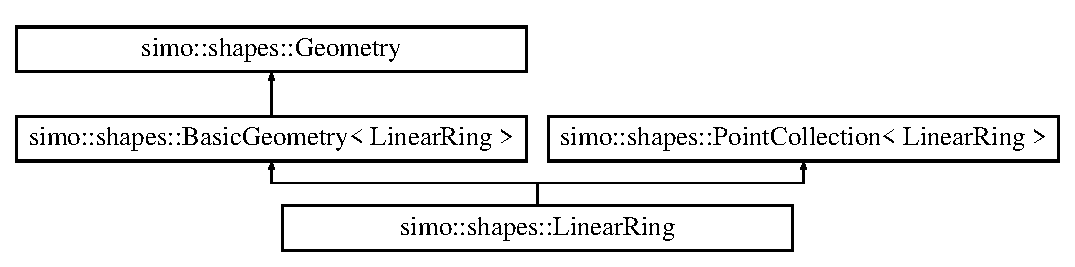
\includegraphics[height=3.000000cm]{classsimo_1_1shapes_1_1_linear_ring}
\end{center}
\end{figure}
\subsection*{Public Member Functions}
\begin{DoxyCompactItemize}
\item 
\hyperlink{classsimo_1_1shapes_1_1_linear_ring_a4d68d8f673858cd04fd281356f3240da}{Linear\-Ring} ()=default
\begin{DoxyCompactList}\small\item\em creates an empty \hyperlink{classsimo_1_1shapes_1_1_linear_ring}{Linear\-Ring} \end{DoxyCompactList}\item 
{\footnotesize template$<$typename T , typename  = typename std\-::enable\-\_\-if$<$std\-::is\-\_\-arithmetic$<$\-T$>$\-::value, T$>$\-::type$>$ }\\\hyperlink{classsimo_1_1shapes_1_1_linear_ring_afdbbd279927592af8eca93cdf9a401c2}{Linear\-Ring} (std\-::initializer\-\_\-list$<$ std\-::initializer\-\_\-list$<$ T $>$$>$ init)
\begin{DoxyCompactList}\small\item\em creates a \hyperlink{classsimo_1_1shapes_1_1_linear_ring}{Linear\-Ring} from a given initializer list \end{DoxyCompactList}\item 
\hyperlink{classsimo_1_1shapes_1_1_linear_ring_a58e04a921d9759ce1ae1c2d4912a4330}{Linear\-Ring} (const std\-::vector$<$ \hyperlink{classsimo_1_1shapes_1_1_point}{Point} $>$ \&points)
\begin{DoxyCompactList}\small\item\em creates a \hyperlink{classsimo_1_1shapes_1_1_linear_ring}{Linear\-Ring} from a given point vector \end{DoxyCompactList}\end{DoxyCompactItemize}
\subsection*{Public Attributes}
\begin{DoxyCompactItemize}
\item 
\hypertarget{classsimo_1_1shapes_1_1_linear_ring_a1bfe68479a45da10f337ba866490528c}{bool \hyperlink{classsimo_1_1shapes_1_1_linear_ring_a1bfe68479a45da10f337ba866490528c}{clockwise} = true}\label{classsimo_1_1shapes_1_1_linear_ring_a1bfe68479a45da10f337ba866490528c}

\begin{DoxyCompactList}\small\item\em two-\/dimensional rotation direction, clockwise=true, counterclockwise=false \end{DoxyCompactList}\end{DoxyCompactItemize}
\subsection*{Additional Inherited Members}


\subsection{Detailed Description}


Definition at line 16 of file linearring.\-hpp.



\subsection{Constructor \& Destructor Documentation}
\hypertarget{classsimo_1_1shapes_1_1_linear_ring_a4d68d8f673858cd04fd281356f3240da}{\index{simo\-::shapes\-::\-Linear\-Ring@{simo\-::shapes\-::\-Linear\-Ring}!Linear\-Ring@{Linear\-Ring}}
\index{Linear\-Ring@{Linear\-Ring}!simo::shapes::LinearRing@{simo\-::shapes\-::\-Linear\-Ring}}
\subsubsection[{Linear\-Ring}]{\setlength{\rightskip}{0pt plus 5cm}simo\-::shapes\-::\-Linear\-Ring\-::\-Linear\-Ring (
\begin{DoxyParamCaption}
{}
\end{DoxyParamCaption}
)\hspace{0.3cm}{\ttfamily [default]}}}\label{classsimo_1_1shapes_1_1_linear_ring_a4d68d8f673858cd04fd281356f3240da}


creates an empty \hyperlink{classsimo_1_1shapes_1_1_linear_ring}{Linear\-Ring} 

\begin{DoxySince}{Since}
0.\-0.\-1 
\end{DoxySince}
\hypertarget{classsimo_1_1shapes_1_1_linear_ring_afdbbd279927592af8eca93cdf9a401c2}{\index{simo\-::shapes\-::\-Linear\-Ring@{simo\-::shapes\-::\-Linear\-Ring}!Linear\-Ring@{Linear\-Ring}}
\index{Linear\-Ring@{Linear\-Ring}!simo::shapes::LinearRing@{simo\-::shapes\-::\-Linear\-Ring}}
\subsubsection[{Linear\-Ring}]{\setlength{\rightskip}{0pt plus 5cm}template$<$typename T , typename  = typename std\-::enable\-\_\-if$<$std\-::is\-\_\-arithmetic$<$\-T$>$\-::value, T$>$\-::type$>$ simo\-::shapes\-::\-Linear\-Ring\-::\-Linear\-Ring (
\begin{DoxyParamCaption}
\item[{std\-::initializer\-\_\-list$<$ std\-::initializer\-\_\-list$<$ T $>$$>$}]{init}
\end{DoxyParamCaption}
)\hspace{0.3cm}{\ttfamily [inline]}}}\label{classsimo_1_1shapes_1_1_linear_ring_afdbbd279927592af8eca93cdf9a401c2}


creates a \hyperlink{classsimo_1_1shapes_1_1_linear_ring}{Linear\-Ring} from a given initializer list 


\begin{DoxyTemplParams}{Template Parameters}
{\em T} & an arithmetic value (e.\-g. int, float, double) \\
\hline
\end{DoxyTemplParams}

\begin{DoxyParams}{Parameters}
{\em init} & the initializer list\\
\hline
\end{DoxyParams}
\begin{DoxySince}{Since}
0.\-0.\-1 
\end{DoxySince}


Definition at line 38 of file linearring.\-hpp.

\hypertarget{classsimo_1_1shapes_1_1_linear_ring_a58e04a921d9759ce1ae1c2d4912a4330}{\index{simo\-::shapes\-::\-Linear\-Ring@{simo\-::shapes\-::\-Linear\-Ring}!Linear\-Ring@{Linear\-Ring}}
\index{Linear\-Ring@{Linear\-Ring}!simo::shapes::LinearRing@{simo\-::shapes\-::\-Linear\-Ring}}
\subsubsection[{Linear\-Ring}]{\setlength{\rightskip}{0pt plus 5cm}simo\-::shapes\-::\-Linear\-Ring\-::\-Linear\-Ring (
\begin{DoxyParamCaption}
\item[{const std\-::vector$<$ {\bf Point} $>$ \&}]{points}
\end{DoxyParamCaption}
)\hspace{0.3cm}{\ttfamily [inline]}, {\ttfamily [explicit]}}}\label{classsimo_1_1shapes_1_1_linear_ring_a58e04a921d9759ce1ae1c2d4912a4330}


creates a \hyperlink{classsimo_1_1shapes_1_1_linear_ring}{Linear\-Ring} from a given point vector 


\begin{DoxyParams}{Parameters}
{\em points} & the point list \\
\hline
{\em validate} & whether to validate the geometry\\
\hline
\end{DoxyParams}
\begin{DoxySince}{Since}
0.\-0.\-1 
\end{DoxySince}


Definition at line 59 of file linearring.\-hpp.



The documentation for this class was generated from the following file\-:\begin{DoxyCompactItemize}
\item 
/home/travis/build/pavelsimo/shapes/include/simo/geom/linearring.\-hpp\end{DoxyCompactItemize}

\hypertarget{classsimo_1_1shapes_1_1_line_string}{\section{simo\-:\-:shapes\-:\-:Line\-String Class Reference}
\label{classsimo_1_1shapes_1_1_line_string}\index{simo\-::shapes\-::\-Line\-String@{simo\-::shapes\-::\-Line\-String}}
}
Inheritance diagram for simo\-:\-:shapes\-:\-:Line\-String\-:\begin{figure}[H]
\begin{center}
\leavevmode
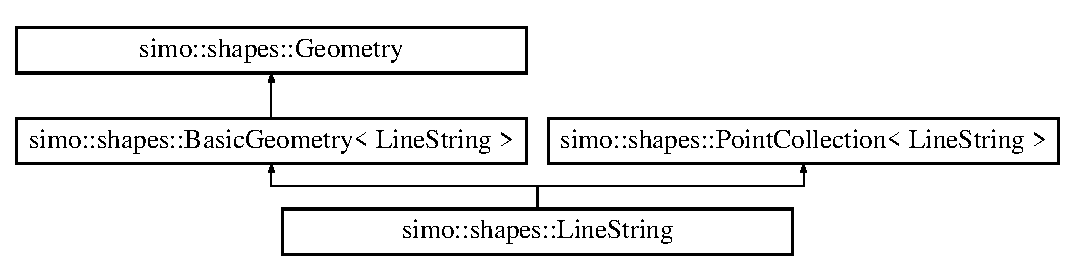
\includegraphics[height=3.000000cm]{classsimo_1_1shapes_1_1_line_string}
\end{center}
\end{figure}
\subsection*{Public Member Functions}
\begin{DoxyCompactItemize}
\item 
\hyperlink{classsimo_1_1shapes_1_1_line_string_ad7af05e6ab868386d3166f81288f7f1c}{Line\-String} ()=default
\begin{DoxyCompactList}\small\item\em creates an empty \hyperlink{classsimo_1_1shapes_1_1_line_string}{Line\-String} \end{DoxyCompactList}\item 
{\footnotesize template$<$typename T , typename  = typename std\-::enable\-\_\-if$<$std\-::is\-\_\-arithmetic$<$\-T$>$\-::value, T$>$\-::type$>$ }\\\hyperlink{classsimo_1_1shapes_1_1_line_string_a25e70d3ca2488e80615bdc0278b231ad}{Line\-String} (std\-::initializer\-\_\-list$<$ std\-::initializer\-\_\-list$<$ T $>$$>$ init)
\begin{DoxyCompactList}\small\item\em creates a \hyperlink{classsimo_1_1shapes_1_1_line_string}{Line\-String} from a given initializer list \end{DoxyCompactList}\item 
\hyperlink{classsimo_1_1shapes_1_1_line_string_a39159fdb1516ed409801499756d627a5}{Line\-String} (const std\-::vector$<$ \hyperlink{classsimo_1_1shapes_1_1_point}{Point} $>$ \&points)
\begin{DoxyCompactList}\small\item\em creates a \hyperlink{classsimo_1_1shapes_1_1_line_string}{Line\-String} from a given point vector \end{DoxyCompactList}\item 
std\-::string \hyperlink{classsimo_1_1shapes_1_1_line_string_a59c052bc895234b68aec25c7d6428e03}{json} ()
\begin{DoxyCompactList}\small\item\em dumps the geojson representation of the \hyperlink{classsimo_1_1shapes_1_1_line_string}{Line\-String} \end{DoxyCompactList}\item 
std\-::string \hyperlink{classsimo_1_1shapes_1_1_line_string_a2e27662b671d0e92df982675f2396492}{wkt} ()
\begin{DoxyCompactList}\small\item\em creates a \hyperlink{classsimo_1_1shapes_1_1_line_string}{Line\-String} from a W\-K\-T string \end{DoxyCompactList}\end{DoxyCompactItemize}
\subsection*{Static Public Member Functions}
\begin{DoxyCompactItemize}
\item 
static \hyperlink{classsimo_1_1shapes_1_1_line_string}{Line\-String} \hyperlink{classsimo_1_1shapes_1_1_line_string_a953c76bf8c908ef9c5c274cd53f39381}{from\-\_\-json} (const std\-::string \&)
\begin{DoxyCompactList}\small\item\em creates a \hyperlink{classsimo_1_1shapes_1_1_line_string}{Line\-String} from a geojson string \end{DoxyCompactList}\item 
static \hyperlink{classsimo_1_1shapes_1_1_line_string}{Line\-String} \hyperlink{classsimo_1_1shapes_1_1_line_string_a348c8ac0e1305c8db575a7fb5c9ca4de}{from\-\_\-wkt} (const std\-::string \&)
\begin{DoxyCompactList}\small\item\em creates a \hyperlink{classsimo_1_1shapes_1_1_line_string}{Line\-String} from a W\-K\-T string \end{DoxyCompactList}\end{DoxyCompactItemize}
\subsection*{Additional Inherited Members}


\subsection{Detailed Description}


Definition at line 16 of file linestring.\-hpp.



\subsection{Constructor \& Destructor Documentation}
\hypertarget{classsimo_1_1shapes_1_1_line_string_ad7af05e6ab868386d3166f81288f7f1c}{\index{simo\-::shapes\-::\-Line\-String@{simo\-::shapes\-::\-Line\-String}!Line\-String@{Line\-String}}
\index{Line\-String@{Line\-String}!simo::shapes::LineString@{simo\-::shapes\-::\-Line\-String}}
\subsubsection[{Line\-String}]{\setlength{\rightskip}{0pt plus 5cm}simo\-::shapes\-::\-Line\-String\-::\-Line\-String (
\begin{DoxyParamCaption}
{}
\end{DoxyParamCaption}
)\hspace{0.3cm}{\ttfamily [default]}}}\label{classsimo_1_1shapes_1_1_line_string_ad7af05e6ab868386d3166f81288f7f1c}


creates an empty \hyperlink{classsimo_1_1shapes_1_1_line_string}{Line\-String} 

\begin{DoxySince}{Since}
0.\-0.\-1 
\end{DoxySince}
\hypertarget{classsimo_1_1shapes_1_1_line_string_a25e70d3ca2488e80615bdc0278b231ad}{\index{simo\-::shapes\-::\-Line\-String@{simo\-::shapes\-::\-Line\-String}!Line\-String@{Line\-String}}
\index{Line\-String@{Line\-String}!simo::shapes::LineString@{simo\-::shapes\-::\-Line\-String}}
\subsubsection[{Line\-String}]{\setlength{\rightskip}{0pt plus 5cm}template$<$typename T , typename  = typename std\-::enable\-\_\-if$<$std\-::is\-\_\-arithmetic$<$\-T$>$\-::value, T$>$\-::type$>$ simo\-::shapes\-::\-Line\-String\-::\-Line\-String (
\begin{DoxyParamCaption}
\item[{std\-::initializer\-\_\-list$<$ std\-::initializer\-\_\-list$<$ T $>$$>$}]{init}
\end{DoxyParamCaption}
)\hspace{0.3cm}{\ttfamily [inline]}}}\label{classsimo_1_1shapes_1_1_line_string_a25e70d3ca2488e80615bdc0278b231ad}


creates a \hyperlink{classsimo_1_1shapes_1_1_line_string}{Line\-String} from a given initializer list 


\begin{DoxyTemplParams}{Template Parameters}
{\em T} & an arithmetic value (e.\-g. int, float, double) \\
\hline
\end{DoxyTemplParams}

\begin{DoxyParams}{Parameters}
{\em init} & the initializer list\\
\hline
\end{DoxyParams}
\begin{DoxySince}{Since}
0.\-0.\-1 
\end{DoxySince}


Definition at line 35 of file linestring.\-hpp.

\hypertarget{classsimo_1_1shapes_1_1_line_string_a39159fdb1516ed409801499756d627a5}{\index{simo\-::shapes\-::\-Line\-String@{simo\-::shapes\-::\-Line\-String}!Line\-String@{Line\-String}}
\index{Line\-String@{Line\-String}!simo::shapes::LineString@{simo\-::shapes\-::\-Line\-String}}
\subsubsection[{Line\-String}]{\setlength{\rightskip}{0pt plus 5cm}simo\-::shapes\-::\-Line\-String\-::\-Line\-String (
\begin{DoxyParamCaption}
\item[{const std\-::vector$<$ {\bf Point} $>$ \&}]{points}
\end{DoxyParamCaption}
)\hspace{0.3cm}{\ttfamily [inline]}, {\ttfamily [explicit]}}}\label{classsimo_1_1shapes_1_1_line_string_a39159fdb1516ed409801499756d627a5}


creates a \hyperlink{classsimo_1_1shapes_1_1_line_string}{Line\-String} from a given point vector 


\begin{DoxyParams}{Parameters}
{\em points} & the point list\\
\hline
\end{DoxyParams}
\begin{DoxySince}{Since}
0.\-0.\-1 
\end{DoxySince}


Definition at line 55 of file linestring.\-hpp.



\subsection{Member Function Documentation}
\hypertarget{classsimo_1_1shapes_1_1_line_string_a953c76bf8c908ef9c5c274cd53f39381}{\index{simo\-::shapes\-::\-Line\-String@{simo\-::shapes\-::\-Line\-String}!from\-\_\-json@{from\-\_\-json}}
\index{from\-\_\-json@{from\-\_\-json}!simo::shapes::LineString@{simo\-::shapes\-::\-Line\-String}}
\subsubsection[{from\-\_\-json}]{\setlength{\rightskip}{0pt plus 5cm}static {\bf Line\-String} simo\-::shapes\-::\-Line\-String\-::from\-\_\-json (
\begin{DoxyParamCaption}
\item[{const std\-::string \&}]{}
\end{DoxyParamCaption}
)\hspace{0.3cm}{\ttfamily [inline]}, {\ttfamily [static]}}}\label{classsimo_1_1shapes_1_1_line_string_a953c76bf8c908ef9c5c274cd53f39381}


creates a \hyperlink{classsimo_1_1shapes_1_1_line_string}{Line\-String} from a geojson string 


\begin{DoxyParams}{Parameters}
{\em json} & the geojson string \\
\hline
\end{DoxyParams}
\begin{DoxyReturn}{Returns}
a \hyperlink{classsimo_1_1shapes_1_1_line_string}{Line\-String} object
\end{DoxyReturn}
\begin{DoxyNote}{Note}
R\-F\-C7946 \href{https://tools.ietf.org/html/rfc7946}{\tt https\-://tools.\-ietf.\-org/html/rfc7946}
\end{DoxyNote}
\begin{DoxySince}{Since}
0.\-0.\-1 
\end{DoxySince}


Definition at line 86 of file linestring.\-hpp.

\hypertarget{classsimo_1_1shapes_1_1_line_string_a348c8ac0e1305c8db575a7fb5c9ca4de}{\index{simo\-::shapes\-::\-Line\-String@{simo\-::shapes\-::\-Line\-String}!from\-\_\-wkt@{from\-\_\-wkt}}
\index{from\-\_\-wkt@{from\-\_\-wkt}!simo::shapes::LineString@{simo\-::shapes\-::\-Line\-String}}
\subsubsection[{from\-\_\-wkt}]{\setlength{\rightskip}{0pt plus 5cm}static {\bf Line\-String} simo\-::shapes\-::\-Line\-String\-::from\-\_\-wkt (
\begin{DoxyParamCaption}
\item[{const std\-::string \&}]{}
\end{DoxyParamCaption}
)\hspace{0.3cm}{\ttfamily [inline]}, {\ttfamily [static]}}}\label{classsimo_1_1shapes_1_1_line_string_a348c8ac0e1305c8db575a7fb5c9ca4de}


creates a \hyperlink{classsimo_1_1shapes_1_1_line_string}{Line\-String} from a W\-K\-T string 


\begin{DoxyParams}{Parameters}
{\em wkt} & the W\-K\-T string \\
\hline
\end{DoxyParams}
\begin{DoxyReturn}{Returns}
a \hyperlink{classsimo_1_1shapes_1_1_line_string}{Line\-String} object
\end{DoxyReturn}
\begin{DoxyNote}{Note}
W\-K\-T \href{https://en.wikipedia.org/wiki/Well-known_text_representation_of_geometry}{\tt https\-://en.\-wikipedia.\-org/wiki/\-Well-\/known\-\_\-text\-\_\-representation\-\_\-of\-\_\-geometry}
\end{DoxyNote}
\begin{DoxySince}{Since}
0.\-0.\-1 
\end{DoxySince}


Definition at line 115 of file linestring.\-hpp.

\hypertarget{classsimo_1_1shapes_1_1_line_string_a59c052bc895234b68aec25c7d6428e03}{\index{simo\-::shapes\-::\-Line\-String@{simo\-::shapes\-::\-Line\-String}!json@{json}}
\index{json@{json}!simo::shapes::LineString@{simo\-::shapes\-::\-Line\-String}}
\subsubsection[{json}]{\setlength{\rightskip}{0pt plus 5cm}std\-::string simo\-::shapes\-::\-Line\-String\-::json (
\begin{DoxyParamCaption}
{}
\end{DoxyParamCaption}
)\hspace{0.3cm}{\ttfamily [inline]}}}\label{classsimo_1_1shapes_1_1_line_string_a59c052bc895234b68aec25c7d6428e03}


dumps the geojson representation of the \hyperlink{classsimo_1_1shapes_1_1_line_string}{Line\-String} 

\begin{DoxyNote}{Note}
R\-F\-C7946 \href{https://tools.ietf.org/html/rfc7946}{\tt https\-://tools.\-ietf.\-org/html/rfc7946}
\end{DoxyNote}
\begin{DoxyReturn}{Returns}
a geojson string
\end{DoxyReturn}
\begin{DoxySince}{Since}
0.\-0.\-1 
\end{DoxySince}


Definition at line 100 of file linestring.\-hpp.

\hypertarget{classsimo_1_1shapes_1_1_line_string_a2e27662b671d0e92df982675f2396492}{\index{simo\-::shapes\-::\-Line\-String@{simo\-::shapes\-::\-Line\-String}!wkt@{wkt}}
\index{wkt@{wkt}!simo::shapes::LineString@{simo\-::shapes\-::\-Line\-String}}
\subsubsection[{wkt}]{\setlength{\rightskip}{0pt plus 5cm}std\-::string simo\-::shapes\-::\-Line\-String\-::wkt (
\begin{DoxyParamCaption}
{}
\end{DoxyParamCaption}
)\hspace{0.3cm}{\ttfamily [inline]}}}\label{classsimo_1_1shapes_1_1_line_string_a2e27662b671d0e92df982675f2396492}


creates a \hyperlink{classsimo_1_1shapes_1_1_line_string}{Line\-String} from a W\-K\-T string 


\begin{DoxyParams}{Parameters}
{\em wkt} & the W\-K\-T string \\
\hline
\end{DoxyParams}
\begin{DoxyReturn}{Returns}
a \hyperlink{classsimo_1_1shapes_1_1_line_string}{Line\-String} object
\end{DoxyReturn}
\begin{DoxyNote}{Note}
W\-K\-T \href{https://en.wikipedia.org/wiki/Well-known_text_representation_of_geometry}{\tt https\-://en.\-wikipedia.\-org/wiki/\-Well-\/known\-\_\-text\-\_\-representation\-\_\-of\-\_\-geometry}
\end{DoxyNote}
\begin{DoxySince}{Since}
0.\-0.\-1 
\end{DoxySince}


Definition at line 130 of file linestring.\-hpp.



The documentation for this class was generated from the following file\-:\begin{DoxyCompactItemize}
\item 
/home/travis/build/pavelsimo/shapes/include/simo/geom/linestring.\-hpp\end{DoxyCompactItemize}

\hypertarget{classsimo_1_1shapes_1_1_multi_point}{\section{simo\-:\-:shapes\-:\-:Multi\-Point Class Reference}
\label{classsimo_1_1shapes_1_1_multi_point}\index{simo\-::shapes\-::\-Multi\-Point@{simo\-::shapes\-::\-Multi\-Point}}
}
Inheritance diagram for simo\-:\-:shapes\-:\-:Multi\-Point\-:\begin{figure}[H]
\begin{center}
\leavevmode
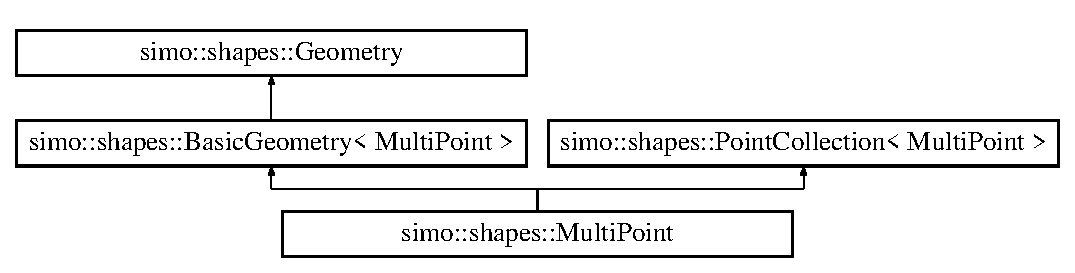
\includegraphics[height=3.000000cm]{classsimo_1_1shapes_1_1_multi_point}
\end{center}
\end{figure}
\subsection*{Public Member Functions}
\begin{DoxyCompactItemize}
\item 
\hyperlink{classsimo_1_1shapes_1_1_multi_point_ad1b9a1a947d02773d9b9cbe18bfdeb12}{Multi\-Point} ()=default
\begin{DoxyCompactList}\small\item\em creates an empty \hyperlink{classsimo_1_1shapes_1_1_multi_point}{Multi\-Point} \end{DoxyCompactList}\item 
{\footnotesize template$<$typename T , typename  = typename std\-::enable\-\_\-if$<$std\-::is\-\_\-arithmetic$<$\-T$>$\-::value, T$>$\-::type$>$ }\\\hyperlink{classsimo_1_1shapes_1_1_multi_point_a5e6cdc0462e2f78395b7c35375ac2afc}{Multi\-Point} (std\-::initializer\-\_\-list$<$ std\-::initializer\-\_\-list$<$ T $>$$>$ init)
\begin{DoxyCompactList}\small\item\em creates a \hyperlink{classsimo_1_1shapes_1_1_multi_point}{Multi\-Point} from a given initializer list \end{DoxyCompactList}\item 
\hyperlink{classsimo_1_1shapes_1_1_multi_point_a894ec2130ac7e5ba82fef72e3b922e0d}{Multi\-Point} (const std\-::vector$<$ \hyperlink{classsimo_1_1shapes_1_1_point}{Point} $>$ \&points)
\begin{DoxyCompactList}\small\item\em creates a \hyperlink{classsimo_1_1shapes_1_1_multi_point}{Multi\-Point} from a given point vector \end{DoxyCompactList}\item 
std\-::string \hyperlink{classsimo_1_1shapes_1_1_multi_point_af802dae29d3887bec0c6bf3687b4b763}{json} ()
\begin{DoxyCompactList}\small\item\em dumps the geojson representation of the \hyperlink{classsimo_1_1shapes_1_1_multi_point}{Multi\-Point} \end{DoxyCompactList}\item 
std\-::string \hyperlink{classsimo_1_1shapes_1_1_multi_point_ae1b037c5687d7629cbb43cfe9700c36a}{wkt} ()
\begin{DoxyCompactList}\small\item\em creates a \hyperlink{classsimo_1_1shapes_1_1_multi_point}{Multi\-Point} from a W\-K\-T string \end{DoxyCompactList}\end{DoxyCompactItemize}
\subsection*{Static Public Member Functions}
\begin{DoxyCompactItemize}
\item 
static \hyperlink{classsimo_1_1shapes_1_1_multi_point}{Multi\-Point} \hyperlink{classsimo_1_1shapes_1_1_multi_point_ad71eee3b464ab12df6e244a63a740e16}{from\-\_\-json} (const std\-::string \&\hyperlink{classsimo_1_1shapes_1_1_multi_point_af802dae29d3887bec0c6bf3687b4b763}{json})
\begin{DoxyCompactList}\small\item\em creates a \hyperlink{classsimo_1_1shapes_1_1_multi_point}{Multi\-Point} from a geojson string \end{DoxyCompactList}\item 
static \hyperlink{classsimo_1_1shapes_1_1_multi_point}{Multi\-Point} \hyperlink{classsimo_1_1shapes_1_1_multi_point_a3a4b2f9eb28019af7c4502a73394783c}{from\-\_\-wkt} (const std\-::string \&)
\begin{DoxyCompactList}\small\item\em creates a \hyperlink{classsimo_1_1shapes_1_1_multi_point}{Multi\-Point} from a W\-K\-T string \end{DoxyCompactList}\end{DoxyCompactItemize}
\subsection*{Additional Inherited Members}


\subsection{Detailed Description}


Definition at line 16 of file multipoint.\-hpp.



\subsection{Constructor \& Destructor Documentation}
\hypertarget{classsimo_1_1shapes_1_1_multi_point_ad1b9a1a947d02773d9b9cbe18bfdeb12}{\index{simo\-::shapes\-::\-Multi\-Point@{simo\-::shapes\-::\-Multi\-Point}!Multi\-Point@{Multi\-Point}}
\index{Multi\-Point@{Multi\-Point}!simo::shapes::MultiPoint@{simo\-::shapes\-::\-Multi\-Point}}
\subsubsection[{Multi\-Point}]{\setlength{\rightskip}{0pt plus 5cm}simo\-::shapes\-::\-Multi\-Point\-::\-Multi\-Point (
\begin{DoxyParamCaption}
{}
\end{DoxyParamCaption}
)\hspace{0.3cm}{\ttfamily [default]}}}\label{classsimo_1_1shapes_1_1_multi_point_ad1b9a1a947d02773d9b9cbe18bfdeb12}


creates an empty \hyperlink{classsimo_1_1shapes_1_1_multi_point}{Multi\-Point} 

\begin{DoxySince}{Since}
0.\-0.\-1 
\end{DoxySince}
\hypertarget{classsimo_1_1shapes_1_1_multi_point_a5e6cdc0462e2f78395b7c35375ac2afc}{\index{simo\-::shapes\-::\-Multi\-Point@{simo\-::shapes\-::\-Multi\-Point}!Multi\-Point@{Multi\-Point}}
\index{Multi\-Point@{Multi\-Point}!simo::shapes::MultiPoint@{simo\-::shapes\-::\-Multi\-Point}}
\subsubsection[{Multi\-Point}]{\setlength{\rightskip}{0pt plus 5cm}template$<$typename T , typename  = typename std\-::enable\-\_\-if$<$std\-::is\-\_\-arithmetic$<$\-T$>$\-::value, T$>$\-::type$>$ simo\-::shapes\-::\-Multi\-Point\-::\-Multi\-Point (
\begin{DoxyParamCaption}
\item[{std\-::initializer\-\_\-list$<$ std\-::initializer\-\_\-list$<$ T $>$$>$}]{init}
\end{DoxyParamCaption}
)\hspace{0.3cm}{\ttfamily [inline]}}}\label{classsimo_1_1shapes_1_1_multi_point_a5e6cdc0462e2f78395b7c35375ac2afc}


creates a \hyperlink{classsimo_1_1shapes_1_1_multi_point}{Multi\-Point} from a given initializer list 


\begin{DoxyTemplParams}{Template Parameters}
{\em T} & an arithmetic value (e.\-g. int, float, double) \\
\hline
\end{DoxyTemplParams}

\begin{DoxyParams}{Parameters}
{\em init} & the initializer list\\
\hline
\end{DoxyParams}
\begin{DoxySince}{Since}
0.\-0.\-1 
\end{DoxySince}


Definition at line 35 of file multipoint.\-hpp.

\hypertarget{classsimo_1_1shapes_1_1_multi_point_a894ec2130ac7e5ba82fef72e3b922e0d}{\index{simo\-::shapes\-::\-Multi\-Point@{simo\-::shapes\-::\-Multi\-Point}!Multi\-Point@{Multi\-Point}}
\index{Multi\-Point@{Multi\-Point}!simo::shapes::MultiPoint@{simo\-::shapes\-::\-Multi\-Point}}
\subsubsection[{Multi\-Point}]{\setlength{\rightskip}{0pt plus 5cm}simo\-::shapes\-::\-Multi\-Point\-::\-Multi\-Point (
\begin{DoxyParamCaption}
\item[{const std\-::vector$<$ {\bf Point} $>$ \&}]{points}
\end{DoxyParamCaption}
)\hspace{0.3cm}{\ttfamily [inline]}, {\ttfamily [explicit]}}}\label{classsimo_1_1shapes_1_1_multi_point_a894ec2130ac7e5ba82fef72e3b922e0d}


creates a \hyperlink{classsimo_1_1shapes_1_1_multi_point}{Multi\-Point} from a given point vector 


\begin{DoxyParams}{Parameters}
{\em points} & the point list\\
\hline
\end{DoxyParams}
\begin{DoxySince}{Since}
0.\-0.\-1 
\end{DoxySince}


Definition at line 54 of file multipoint.\-hpp.



\subsection{Member Function Documentation}
\hypertarget{classsimo_1_1shapes_1_1_multi_point_ad71eee3b464ab12df6e244a63a740e16}{\index{simo\-::shapes\-::\-Multi\-Point@{simo\-::shapes\-::\-Multi\-Point}!from\-\_\-json@{from\-\_\-json}}
\index{from\-\_\-json@{from\-\_\-json}!simo::shapes::MultiPoint@{simo\-::shapes\-::\-Multi\-Point}}
\subsubsection[{from\-\_\-json}]{\setlength{\rightskip}{0pt plus 5cm}static {\bf Multi\-Point} simo\-::shapes\-::\-Multi\-Point\-::from\-\_\-json (
\begin{DoxyParamCaption}
\item[{const std\-::string \&}]{json}
\end{DoxyParamCaption}
)\hspace{0.3cm}{\ttfamily [inline]}, {\ttfamily [static]}}}\label{classsimo_1_1shapes_1_1_multi_point_ad71eee3b464ab12df6e244a63a740e16}


creates a \hyperlink{classsimo_1_1shapes_1_1_multi_point}{Multi\-Point} from a geojson string 


\begin{DoxyParams}{Parameters}
{\em json} & the geojson string \\
\hline
\end{DoxyParams}
\begin{DoxyReturn}{Returns}
a \hyperlink{classsimo_1_1shapes_1_1_multi_point}{Multi\-Point} object
\end{DoxyReturn}
\begin{DoxyNote}{Note}
R\-F\-C7946 \href{https://tools.ietf.org/html/rfc7946}{\tt https\-://tools.\-ietf.\-org/html/rfc7946}
\end{DoxyNote}
\begin{DoxySince}{Since}
0.\-0.\-1 
\end{DoxySince}
\begin{DoxyRefDesc}{Todo}
\item[\hyperlink{todo__todo000006}{Todo}](pavel) read properties to specify z, m and zm \end{DoxyRefDesc}


Definition at line 90 of file multipoint.\-hpp.

\hypertarget{classsimo_1_1shapes_1_1_multi_point_a3a4b2f9eb28019af7c4502a73394783c}{\index{simo\-::shapes\-::\-Multi\-Point@{simo\-::shapes\-::\-Multi\-Point}!from\-\_\-wkt@{from\-\_\-wkt}}
\index{from\-\_\-wkt@{from\-\_\-wkt}!simo::shapes::MultiPoint@{simo\-::shapes\-::\-Multi\-Point}}
\subsubsection[{from\-\_\-wkt}]{\setlength{\rightskip}{0pt plus 5cm}static {\bf Multi\-Point} simo\-::shapes\-::\-Multi\-Point\-::from\-\_\-wkt (
\begin{DoxyParamCaption}
\item[{const std\-::string \&}]{}
\end{DoxyParamCaption}
)\hspace{0.3cm}{\ttfamily [inline]}, {\ttfamily [static]}}}\label{classsimo_1_1shapes_1_1_multi_point_a3a4b2f9eb28019af7c4502a73394783c}


creates a \hyperlink{classsimo_1_1shapes_1_1_multi_point}{Multi\-Point} from a W\-K\-T string 


\begin{DoxyParams}{Parameters}
{\em wkt} & the W\-K\-T string \\
\hline
\end{DoxyParams}
\begin{DoxyReturn}{Returns}
a \hyperlink{classsimo_1_1shapes_1_1_multi_point}{Multi\-Point} object
\end{DoxyReturn}
\begin{DoxyNote}{Note}
W\-K\-T \href{https://en.wikipedia.org/wiki/Well-known_text_representation_of_geometry}{\tt https\-://en.\-wikipedia.\-org/wiki/\-Well-\/known\-\_\-text\-\_\-representation\-\_\-of\-\_\-geometry}
\end{DoxyNote}
\begin{DoxySince}{Since}
0.\-0.\-1 
\end{DoxySince}


Definition at line 180 of file multipoint.\-hpp.

\hypertarget{classsimo_1_1shapes_1_1_multi_point_af802dae29d3887bec0c6bf3687b4b763}{\index{simo\-::shapes\-::\-Multi\-Point@{simo\-::shapes\-::\-Multi\-Point}!json@{json}}
\index{json@{json}!simo::shapes::MultiPoint@{simo\-::shapes\-::\-Multi\-Point}}
\subsubsection[{json}]{\setlength{\rightskip}{0pt plus 5cm}std\-::string simo\-::shapes\-::\-Multi\-Point\-::json (
\begin{DoxyParamCaption}
{}
\end{DoxyParamCaption}
)\hspace{0.3cm}{\ttfamily [inline]}}}\label{classsimo_1_1shapes_1_1_multi_point_af802dae29d3887bec0c6bf3687b4b763}


dumps the geojson representation of the \hyperlink{classsimo_1_1shapes_1_1_multi_point}{Multi\-Point} 

\begin{DoxyNote}{Note}
R\-F\-C7946 \href{https://tools.ietf.org/html/rfc7946}{\tt https\-://tools.\-ietf.\-org/html/rfc7946}
\end{DoxyNote}
\begin{DoxyReturn}{Returns}
a geojson string
\end{DoxyReturn}
\begin{DoxySince}{Since}
0.\-0.\-1 
\end{DoxySince}
\begin{DoxyRefDesc}{Todo}
\item[\hyperlink{todo__todo000007}{Todo}](pavel) add properties to specify z, m and zm \end{DoxyRefDesc}


Definition at line 129 of file multipoint.\-hpp.

\hypertarget{classsimo_1_1shapes_1_1_multi_point_ae1b037c5687d7629cbb43cfe9700c36a}{\index{simo\-::shapes\-::\-Multi\-Point@{simo\-::shapes\-::\-Multi\-Point}!wkt@{wkt}}
\index{wkt@{wkt}!simo::shapes::MultiPoint@{simo\-::shapes\-::\-Multi\-Point}}
\subsubsection[{wkt}]{\setlength{\rightskip}{0pt plus 5cm}std\-::string simo\-::shapes\-::\-Multi\-Point\-::wkt (
\begin{DoxyParamCaption}
{}
\end{DoxyParamCaption}
)\hspace{0.3cm}{\ttfamily [inline]}}}\label{classsimo_1_1shapes_1_1_multi_point_ae1b037c5687d7629cbb43cfe9700c36a}


creates a \hyperlink{classsimo_1_1shapes_1_1_multi_point}{Multi\-Point} from a W\-K\-T string 


\begin{DoxyParams}{Parameters}
{\em wkt} & the W\-K\-T string \\
\hline
\end{DoxyParams}
\begin{DoxyReturn}{Returns}
a \hyperlink{classsimo_1_1shapes_1_1_multi_point}{Multi\-Point} object
\end{DoxyReturn}
\begin{DoxyNote}{Note}
W\-K\-T \href{https://en.wikipedia.org/wiki/Well-known_text_representation_of_geometry}{\tt https\-://en.\-wikipedia.\-org/wiki/\-Well-\/known\-\_\-text\-\_\-representation\-\_\-of\-\_\-geometry}
\end{DoxyNote}
\begin{DoxySince}{Since}
0.\-0.\-1 
\end{DoxySince}


Definition at line 196 of file multipoint.\-hpp.



The documentation for this class was generated from the following file\-:\begin{DoxyCompactItemize}
\item 
/home/travis/build/pavelsimo/shapes/include/simo/geom/multipoint.\-hpp\end{DoxyCompactItemize}

\hypertarget{classsimo_1_1shapes_1_1exceptions_1_1not__implemented__error}{\section{simo\-:\-:shapes\-:\-:exceptions\-:\-:not\-\_\-implemented\-\_\-error Class Reference}
\label{classsimo_1_1shapes_1_1exceptions_1_1not__implemented__error}\index{simo\-::shapes\-::exceptions\-::not\-\_\-implemented\-\_\-error@{simo\-::shapes\-::exceptions\-::not\-\_\-implemented\-\_\-error}}
}


{\ttfamily \#include $<$exceptions.\-hpp$>$}

Inheritance diagram for simo\-:\-:shapes\-:\-:exceptions\-:\-:not\-\_\-implemented\-\_\-error\-:\begin{figure}[H]
\begin{center}
\leavevmode
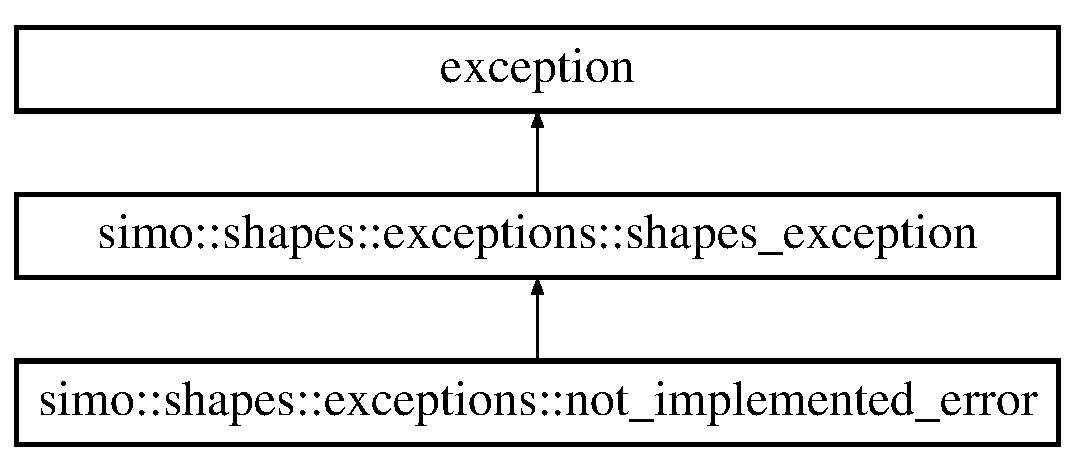
\includegraphics[height=3.000000cm]{classsimo_1_1shapes_1_1exceptions_1_1not__implemented__error}
\end{center}
\end{figure}
\subsection*{Public Member Functions}
\begin{DoxyCompactItemize}
\item 
\hypertarget{classsimo_1_1shapes_1_1exceptions_1_1not__implemented__error_aee69f5e86b7f01af95e7fedda1b9e10c}{{\bfseries not\-\_\-implemented\-\_\-error} (const std\-::string \&reason)}\label{classsimo_1_1shapes_1_1exceptions_1_1not__implemented__error_aee69f5e86b7f01af95e7fedda1b9e10c}

\end{DoxyCompactItemize}
\subsection*{Additional Inherited Members}


\subsection{Detailed Description}
\begin{DoxyRefDesc}{Todo}
\item[\hyperlink{todo__todo000002}{Todo}](pavel) D\-O\-C\-U\-M\-E\-N\-T M\-E! \end{DoxyRefDesc}


Definition at line 54 of file exceptions.\-hpp.



The documentation for this class was generated from the following file\-:\begin{DoxyCompactItemize}
\item 
/home/travis/build/pavelsimo/shapes/include/simo/exceptions.\-hpp\end{DoxyCompactItemize}

\hypertarget{classsimo_1_1shapes_1_1exceptions_1_1parse__error}{\section{simo\-:\-:shapes\-:\-:exceptions\-:\-:parse\-\_\-error Class Reference}
\label{classsimo_1_1shapes_1_1exceptions_1_1parse__error}\index{simo\-::shapes\-::exceptions\-::parse\-\_\-error@{simo\-::shapes\-::exceptions\-::parse\-\_\-error}}
}


{\ttfamily \#include $<$exceptions.\-hpp$>$}

Inheritance diagram for simo\-:\-:shapes\-:\-:exceptions\-:\-:parse\-\_\-error\-:\begin{figure}[H]
\begin{center}
\leavevmode
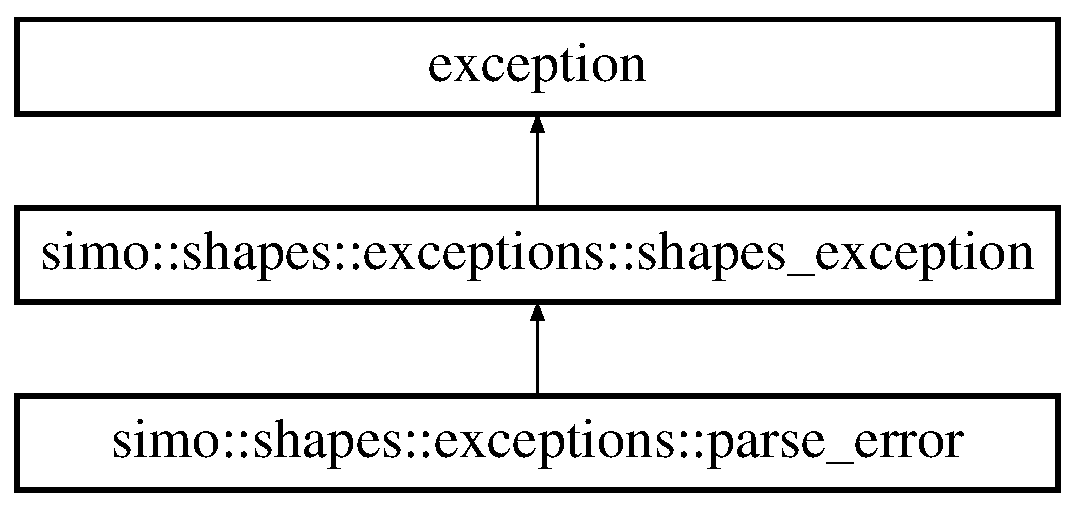
\includegraphics[height=3.000000cm]{classsimo_1_1shapes_1_1exceptions_1_1parse__error}
\end{center}
\end{figure}
\subsection*{Public Member Functions}
\begin{DoxyCompactItemize}
\item 
\hypertarget{classsimo_1_1shapes_1_1exceptions_1_1parse__error_ab17b7f0934ad6fee8a0ca1acae4ad7d5}{{\bfseries parse\-\_\-error} (const std\-::string \&reason)}\label{classsimo_1_1shapes_1_1exceptions_1_1parse__error_ab17b7f0934ad6fee8a0ca1acae4ad7d5}

\end{DoxyCompactItemize}
\subsection*{Additional Inherited Members}


\subsection{Detailed Description}
\begin{DoxyRefDesc}{Todo}
\item[\hyperlink{todo__todo000001}{Todo}](pavel) D\-O\-C\-U\-M\-E\-N\-T M\-E! \end{DoxyRefDesc}


Definition at line 41 of file exceptions.\-hpp.



The documentation for this class was generated from the following file\-:\begin{DoxyCompactItemize}
\item 
/home/travis/build/pavelsimo/shapes/include/simo/exceptions.\-hpp\end{DoxyCompactItemize}

\hypertarget{classsimo_1_1shapes_1_1_point}{\section{simo\-:\-:shapes\-:\-:Point Class Reference}
\label{classsimo_1_1shapes_1_1_point}\index{simo\-::shapes\-::\-Point@{simo\-::shapes\-::\-Point}}
}
Inheritance diagram for simo\-:\-:shapes\-:\-:Point\-:\begin{figure}[H]
\begin{center}
\leavevmode
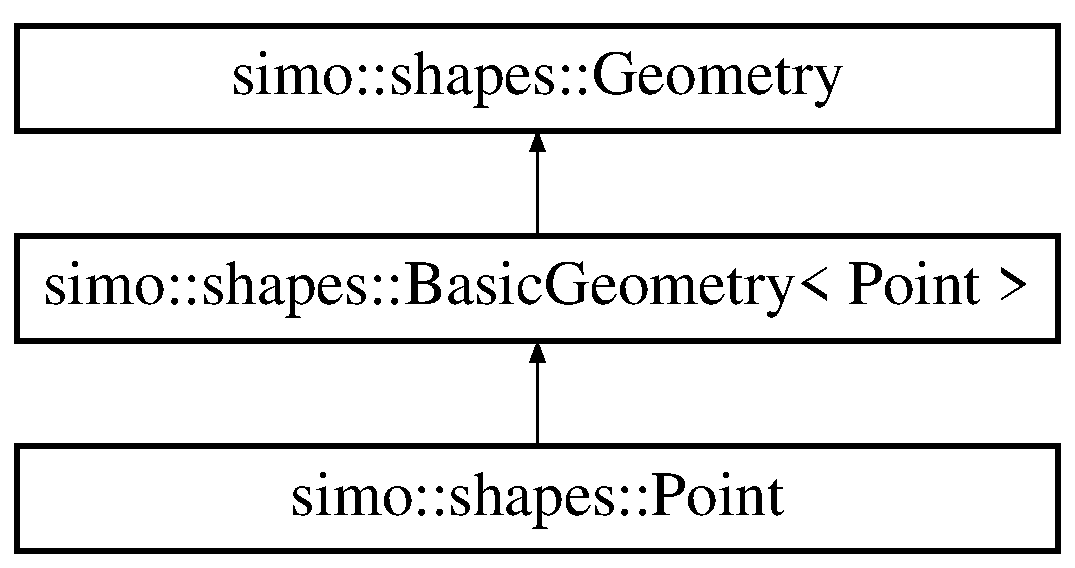
\includegraphics[height=3.000000cm]{classsimo_1_1shapes_1_1_point}
\end{center}
\end{figure}
\subsection*{Public Member Functions}
\begin{DoxyCompactItemize}
\item 
\hyperlink{classsimo_1_1shapes_1_1_point_a754115ccb65d25bc28dadee1d62f5955}{Point} ()
\begin{DoxyCompactList}\small\item\em creates a \hyperlink{classsimo_1_1shapes_1_1_point}{Point} \end{DoxyCompactList}\item 
\hyperlink{classsimo_1_1shapes_1_1_point_a4932bd8b5eeccc1767de9bfb2f65f1c3}{Point} (double \hyperlink{classsimo_1_1shapes_1_1_point_aa4abc96b03859b69bb1af19099a9799f}{x}, double \hyperlink{classsimo_1_1shapes_1_1_point_a370ca8d7d03517735a9792cca7cbb05e}{y})
\begin{DoxyCompactList}\small\item\em creates a \hyperlink{classsimo_1_1shapes_1_1_point}{Point} from coordinates (x, y) \end{DoxyCompactList}\item 
\hyperlink{classsimo_1_1shapes_1_1_point_ac1c250658a3cc7bee49ec49c57431d7a}{Point} (double \hyperlink{classsimo_1_1shapes_1_1_point_aa4abc96b03859b69bb1af19099a9799f}{x}, double \hyperlink{classsimo_1_1shapes_1_1_point_a370ca8d7d03517735a9792cca7cbb05e}{y}, double \hyperlink{classsimo_1_1shapes_1_1_point_a4498c1e84bb25e32cd75d41a74d48169}{z})
\begin{DoxyCompactList}\small\item\em creates a \hyperlink{classsimo_1_1shapes_1_1_point}{Point} from coordinates (x, y, z) \end{DoxyCompactList}\item 
\hyperlink{classsimo_1_1shapes_1_1_point_a30ce91412930c35da44537bd8b5a6ea1}{Point} (double \hyperlink{classsimo_1_1shapes_1_1_point_aa4abc96b03859b69bb1af19099a9799f}{x}, double \hyperlink{classsimo_1_1shapes_1_1_point_a370ca8d7d03517735a9792cca7cbb05e}{y}, double \hyperlink{classsimo_1_1shapes_1_1_point_a4498c1e84bb25e32cd75d41a74d48169}{z}, double \hyperlink{classsimo_1_1shapes_1_1_point_aced73731924b13762c7b6446bf3ad9a5}{m})
\begin{DoxyCompactList}\small\item\em creates a \hyperlink{classsimo_1_1shapes_1_1_point}{Point} from coordinates (x, y, z, m) \end{DoxyCompactList}\item 
{\footnotesize template$<$typename T , typename  = typename std\-::enable\-\_\-if$<$std\-::is\-\_\-arithmetic$<$\-T$>$\-::value, T$>$\-::type$>$ }\\\hyperlink{classsimo_1_1shapes_1_1_point_a8378b498b96e68e341407007a6d69b91}{Point} (std\-::initializer\-\_\-list$<$ T $>$ init)
\begin{DoxyCompactList}\small\item\em creates a \hyperlink{classsimo_1_1shapes_1_1_point}{Point} \end{DoxyCompactList}\item 
double \hyperlink{classsimo_1_1shapes_1_1_point_aac896c5b6bb2ba85442a639e611534df}{at} (size\-\_\-t pos)
\begin{DoxyCompactList}\small\item\em returns the coordinate at the given index \end{DoxyCompactList}\item 
double \hyperlink{classsimo_1_1shapes_1_1_point_a72cdeb0d8d8ecfdd5c5f4da19ec33cc4}{operator\mbox{[}$\,$\mbox{]}} (size\-\_\-t pos)
\begin{DoxyCompactList}\small\item\em returns the coordinate at the given index \end{DoxyCompactList}\item 
bool \hyperlink{classsimo_1_1shapes_1_1_point_a32b64226c96ab13e4b44e7437c2f6b3e}{operator==} (const \hyperlink{classsimo_1_1shapes_1_1_point}{Point} \&other) const 
\item 
bool \hyperlink{classsimo_1_1shapes_1_1_point_aece2f7cb87b1ca009d29fb79fcf8b48a}{operator!=} (const \hyperlink{classsimo_1_1shapes_1_1_point}{Point} \&other) const 
\item 
std\-::string \hyperlink{classsimo_1_1shapes_1_1_point_ab16bf7c8f22a3fbd0df4e8a7407eeda5}{json} ()
\begin{DoxyCompactList}\small\item\em dumps the geojson representation of the \hyperlink{classsimo_1_1shapes_1_1_point}{Point} \end{DoxyCompactList}\item 
std\-::string \hyperlink{classsimo_1_1shapes_1_1_point_a4134ec6fcf72ca4d822a9a70788dee40}{wkt} ()
\begin{DoxyCompactList}\small\item\em dumps the W\-K\-T representation of the point \end{DoxyCompactList}\end{DoxyCompactItemize}
\subsection*{Static Public Member Functions}
\begin{DoxyCompactItemize}
\item 
static \hyperlink{classsimo_1_1shapes_1_1_point}{Point} \hyperlink{classsimo_1_1shapes_1_1_point_a5babfdb4e450381fce0bd355c060d3cf}{from\-\_\-xy} (double \hyperlink{classsimo_1_1shapes_1_1_point_aa4abc96b03859b69bb1af19099a9799f}{x}, double \hyperlink{classsimo_1_1shapes_1_1_point_a370ca8d7d03517735a9792cca7cbb05e}{y})
\begin{DoxyCompactList}\small\item\em creates a \hyperlink{classsimo_1_1shapes_1_1_point}{Point} from coordinates (x, y) \end{DoxyCompactList}\item 
static \hyperlink{classsimo_1_1shapes_1_1_point}{Point} \hyperlink{classsimo_1_1shapes_1_1_point_af2fe59e7e25d3ab1019fbf9a3365fa30}{from\-\_\-xyz} (double \hyperlink{classsimo_1_1shapes_1_1_point_aa4abc96b03859b69bb1af19099a9799f}{x}, double \hyperlink{classsimo_1_1shapes_1_1_point_a370ca8d7d03517735a9792cca7cbb05e}{y}, double \hyperlink{classsimo_1_1shapes_1_1_point_a4498c1e84bb25e32cd75d41a74d48169}{z})
\begin{DoxyCompactList}\small\item\em creates a \hyperlink{classsimo_1_1shapes_1_1_point}{Point} from coordinates (x, y, z) \end{DoxyCompactList}\item 
static \hyperlink{classsimo_1_1shapes_1_1_point}{Point} \hyperlink{classsimo_1_1shapes_1_1_point_a73475fb5d47c0c77506d8c83c0287f57}{from\-\_\-xym} (double \hyperlink{classsimo_1_1shapes_1_1_point_aa4abc96b03859b69bb1af19099a9799f}{x}, double \hyperlink{classsimo_1_1shapes_1_1_point_a370ca8d7d03517735a9792cca7cbb05e}{y}, double \hyperlink{classsimo_1_1shapes_1_1_point_aced73731924b13762c7b6446bf3ad9a5}{m})
\begin{DoxyCompactList}\small\item\em creates a \hyperlink{classsimo_1_1shapes_1_1_point}{Point} from coordinates (x, y, m) \end{DoxyCompactList}\item 
static \hyperlink{classsimo_1_1shapes_1_1_point}{Point} \hyperlink{classsimo_1_1shapes_1_1_point_a04c56d21b56fa034bb9b83150bb89a10}{from\-\_\-xyzm} (double \hyperlink{classsimo_1_1shapes_1_1_point_aa4abc96b03859b69bb1af19099a9799f}{x}, double \hyperlink{classsimo_1_1shapes_1_1_point_a370ca8d7d03517735a9792cca7cbb05e}{y}, double \hyperlink{classsimo_1_1shapes_1_1_point_a4498c1e84bb25e32cd75d41a74d48169}{z}, double \hyperlink{classsimo_1_1shapes_1_1_point_aced73731924b13762c7b6446bf3ad9a5}{m})
\begin{DoxyCompactList}\small\item\em creates a \hyperlink{classsimo_1_1shapes_1_1_point}{Point} from coordinates (x, y, z, m) \end{DoxyCompactList}\item 
static \hyperlink{classsimo_1_1shapes_1_1_point}{Point} \hyperlink{classsimo_1_1shapes_1_1_point_a7de22a22436ff219a0714602d865b723}{from\-\_\-json} (const std\-::string \&\hyperlink{classsimo_1_1shapes_1_1_point_ab16bf7c8f22a3fbd0df4e8a7407eeda5}{json})
\begin{DoxyCompactList}\small\item\em creates a \hyperlink{classsimo_1_1shapes_1_1_point}{Point} from a geojson string \end{DoxyCompactList}\item 
static \hyperlink{classsimo_1_1shapes_1_1_point}{Point} \hyperlink{classsimo_1_1shapes_1_1_point_aa140e02a04b52bf5739a761528dfd8e9}{from\-\_\-wkt} (const std\-::string \&\hyperlink{classsimo_1_1shapes_1_1_point_a4134ec6fcf72ca4d822a9a70788dee40}{wkt})
\begin{DoxyCompactList}\small\item\em creates a \hyperlink{classsimo_1_1shapes_1_1_point}{Point} from a W\-K\-T string \end{DoxyCompactList}\end{DoxyCompactItemize}
\subsection*{Public Attributes}
\begin{DoxyCompactItemize}
\item 
\hypertarget{classsimo_1_1shapes_1_1_point_aa4abc96b03859b69bb1af19099a9799f}{double \hyperlink{classsimo_1_1shapes_1_1_point_aa4abc96b03859b69bb1af19099a9799f}{x} = 0}\label{classsimo_1_1shapes_1_1_point_aa4abc96b03859b69bb1af19099a9799f}

\begin{DoxyCompactList}\small\item\em the x-\/coordinate value for this \hyperlink{classsimo_1_1shapes_1_1_point}{Point} \end{DoxyCompactList}\item 
\hypertarget{classsimo_1_1shapes_1_1_point_a370ca8d7d03517735a9792cca7cbb05e}{double \hyperlink{classsimo_1_1shapes_1_1_point_a370ca8d7d03517735a9792cca7cbb05e}{y} = 0}\label{classsimo_1_1shapes_1_1_point_a370ca8d7d03517735a9792cca7cbb05e}

\begin{DoxyCompactList}\small\item\em the y-\/coordinate value for this \hyperlink{classsimo_1_1shapes_1_1_point}{Point} \end{DoxyCompactList}\item 
\hypertarget{classsimo_1_1shapes_1_1_point_a4498c1e84bb25e32cd75d41a74d48169}{double \hyperlink{classsimo_1_1shapes_1_1_point_a4498c1e84bb25e32cd75d41a74d48169}{z} = 0}\label{classsimo_1_1shapes_1_1_point_a4498c1e84bb25e32cd75d41a74d48169}

\begin{DoxyCompactList}\small\item\em the z-\/coordinate value for this \hyperlink{classsimo_1_1shapes_1_1_point}{Point}, if it has one. \end{DoxyCompactList}\item 
\hypertarget{classsimo_1_1shapes_1_1_point_aced73731924b13762c7b6446bf3ad9a5}{double \hyperlink{classsimo_1_1shapes_1_1_point_aced73731924b13762c7b6446bf3ad9a5}{m} = 0}\label{classsimo_1_1shapes_1_1_point_aced73731924b13762c7b6446bf3ad9a5}

\begin{DoxyCompactList}\small\item\em the m-\/coordinate value for this \hyperlink{classsimo_1_1shapes_1_1_point}{Point}, if it has one. \end{DoxyCompactList}\end{DoxyCompactItemize}


\subsection{Detailed Description}


Definition at line 23 of file point.\-hpp.



\subsection{Constructor \& Destructor Documentation}
\hypertarget{classsimo_1_1shapes_1_1_point_a754115ccb65d25bc28dadee1d62f5955}{\index{simo\-::shapes\-::\-Point@{simo\-::shapes\-::\-Point}!Point@{Point}}
\index{Point@{Point}!simo::shapes::Point@{simo\-::shapes\-::\-Point}}
\subsubsection[{Point}]{\setlength{\rightskip}{0pt plus 5cm}simo\-::shapes\-::\-Point\-::\-Point (
\begin{DoxyParamCaption}
{}
\end{DoxyParamCaption}
)\hspace{0.3cm}{\ttfamily [inline]}}}\label{classsimo_1_1shapes_1_1_point_a754115ccb65d25bc28dadee1d62f5955}


creates a \hyperlink{classsimo_1_1shapes_1_1_point}{Point} 

\begin{DoxyNote}{Note}
the default behaviour is to create a 2-\/dimensional point with coordinates (0, 0)
\end{DoxyNote}
\begin{DoxySince}{Since}
0.\-0.\-1 
\end{DoxySince}


Definition at line 45 of file point.\-hpp.

\hypertarget{classsimo_1_1shapes_1_1_point_a4932bd8b5eeccc1767de9bfb2f65f1c3}{\index{simo\-::shapes\-::\-Point@{simo\-::shapes\-::\-Point}!Point@{Point}}
\index{Point@{Point}!simo::shapes::Point@{simo\-::shapes\-::\-Point}}
\subsubsection[{Point}]{\setlength{\rightskip}{0pt plus 5cm}simo\-::shapes\-::\-Point\-::\-Point (
\begin{DoxyParamCaption}
\item[{double}]{x, }
\item[{double}]{y}
\end{DoxyParamCaption}
)\hspace{0.3cm}{\ttfamily [inline]}}}\label{classsimo_1_1shapes_1_1_point_a4932bd8b5eeccc1767de9bfb2f65f1c3}


creates a \hyperlink{classsimo_1_1shapes_1_1_point}{Point} from coordinates (x, y) 


\begin{DoxyParams}{Parameters}
{\em x} & the x-\/coordinate value \\
\hline
{\em y} & the y-\/coordinate value\\
\hline
\end{DoxyParams}
\begin{DoxySince}{Since}
0.\-0.\-1 
\end{DoxySince}


Definition at line 58 of file point.\-hpp.

\hypertarget{classsimo_1_1shapes_1_1_point_ac1c250658a3cc7bee49ec49c57431d7a}{\index{simo\-::shapes\-::\-Point@{simo\-::shapes\-::\-Point}!Point@{Point}}
\index{Point@{Point}!simo::shapes::Point@{simo\-::shapes\-::\-Point}}
\subsubsection[{Point}]{\setlength{\rightskip}{0pt plus 5cm}simo\-::shapes\-::\-Point\-::\-Point (
\begin{DoxyParamCaption}
\item[{double}]{x, }
\item[{double}]{y, }
\item[{double}]{z}
\end{DoxyParamCaption}
)\hspace{0.3cm}{\ttfamily [inline]}}}\label{classsimo_1_1shapes_1_1_point_ac1c250658a3cc7bee49ec49c57431d7a}


creates a \hyperlink{classsimo_1_1shapes_1_1_point}{Point} from coordinates (x, y, z) 


\begin{DoxyParams}{Parameters}
{\em x} & the x-\/coordinate value \\
\hline
{\em y} & the y-\/coordinate value \\
\hline
{\em z} & the z-\/coordinate value\\
\hline
\end{DoxyParams}
\begin{DoxySince}{Since}
0.\-0.\-1 
\end{DoxySince}


Definition at line 73 of file point.\-hpp.

\hypertarget{classsimo_1_1shapes_1_1_point_a30ce91412930c35da44537bd8b5a6ea1}{\index{simo\-::shapes\-::\-Point@{simo\-::shapes\-::\-Point}!Point@{Point}}
\index{Point@{Point}!simo::shapes::Point@{simo\-::shapes\-::\-Point}}
\subsubsection[{Point}]{\setlength{\rightskip}{0pt plus 5cm}simo\-::shapes\-::\-Point\-::\-Point (
\begin{DoxyParamCaption}
\item[{double}]{x, }
\item[{double}]{y, }
\item[{double}]{z, }
\item[{double}]{m}
\end{DoxyParamCaption}
)\hspace{0.3cm}{\ttfamily [inline]}}}\label{classsimo_1_1shapes_1_1_point_a30ce91412930c35da44537bd8b5a6ea1}


creates a \hyperlink{classsimo_1_1shapes_1_1_point}{Point} from coordinates (x, y, z, m) 


\begin{DoxyParams}{Parameters}
{\em x} & the x-\/coordinate value \\
\hline
{\em y} & the y-\/coordinate value \\
\hline
{\em z} & the z-\/coordinate value \\
\hline
{\em m} & the m-\/coordinate (measure) value\\
\hline
\end{DoxyParams}
\begin{DoxySince}{Since}
0.\-0.\-1 
\end{DoxySince}


Definition at line 89 of file point.\-hpp.

\hypertarget{classsimo_1_1shapes_1_1_point_a8378b498b96e68e341407007a6d69b91}{\index{simo\-::shapes\-::\-Point@{simo\-::shapes\-::\-Point}!Point@{Point}}
\index{Point@{Point}!simo::shapes::Point@{simo\-::shapes\-::\-Point}}
\subsubsection[{Point}]{\setlength{\rightskip}{0pt plus 5cm}template$<$typename T , typename  = typename std\-::enable\-\_\-if$<$std\-::is\-\_\-arithmetic$<$\-T$>$\-::value, T$>$\-::type$>$ simo\-::shapes\-::\-Point\-::\-Point (
\begin{DoxyParamCaption}
\item[{std\-::initializer\-\_\-list$<$ T $>$}]{init}
\end{DoxyParamCaption}
)\hspace{0.3cm}{\ttfamily [inline]}}}\label{classsimo_1_1shapes_1_1_point_a8378b498b96e68e341407007a6d69b91}


creates a \hyperlink{classsimo_1_1shapes_1_1_point}{Point} 


\begin{DoxyTemplParams}{Template Parameters}
{\em T} & an arithmetic value (e.\-g. int, float, double) \\
\hline
\end{DoxyTemplParams}

\begin{DoxyParams}{Parameters}
{\em init} & the coordinates list\\
\hline
\end{DoxyParams}

\begin{DoxyExceptions}{Exceptions}
{\em exception} & if the given number of coordinates is either less than two or greater than four\\
\hline
\end{DoxyExceptions}
\begin{DoxySince}{Since}
0.\-0.\-1 
\end{DoxySince}


Definition at line 167 of file point.\-hpp.



\subsection{Member Function Documentation}
\hypertarget{classsimo_1_1shapes_1_1_point_aac896c5b6bb2ba85442a639e611534df}{\index{simo\-::shapes\-::\-Point@{simo\-::shapes\-::\-Point}!at@{at}}
\index{at@{at}!simo::shapes::Point@{simo\-::shapes\-::\-Point}}
\subsubsection[{at}]{\setlength{\rightskip}{0pt plus 5cm}double simo\-::shapes\-::\-Point\-::at (
\begin{DoxyParamCaption}
\item[{size\-\_\-t}]{pos}
\end{DoxyParamCaption}
)\hspace{0.3cm}{\ttfamily [inline]}}}\label{classsimo_1_1shapes_1_1_point_aac896c5b6bb2ba85442a639e611534df}


returns the coordinate at the given index 


\begin{DoxyParams}{Parameters}
{\em pos} & the coordinate position \\
\hline
\end{DoxyParams}
\begin{DoxyReturn}{Returns}
a double with the coordinate value
\end{DoxyReturn}

\begin{DoxyExceptions}{Exceptions}
{\em exception} & if the position is not found\\
\hline
\end{DoxyExceptions}
\begin{DoxySince}{Since}
0.\-0.\-1 
\end{DoxySince}


Definition at line 262 of file point.\-hpp.

\hypertarget{classsimo_1_1shapes_1_1_point_a7de22a22436ff219a0714602d865b723}{\index{simo\-::shapes\-::\-Point@{simo\-::shapes\-::\-Point}!from\-\_\-json@{from\-\_\-json}}
\index{from\-\_\-json@{from\-\_\-json}!simo::shapes::Point@{simo\-::shapes\-::\-Point}}
\subsubsection[{from\-\_\-json}]{\setlength{\rightskip}{0pt plus 5cm}static {\bf Point} simo\-::shapes\-::\-Point\-::from\-\_\-json (
\begin{DoxyParamCaption}
\item[{const std\-::string \&}]{json}
\end{DoxyParamCaption}
)\hspace{0.3cm}{\ttfamily [inline]}, {\ttfamily [static]}}}\label{classsimo_1_1shapes_1_1_point_a7de22a22436ff219a0714602d865b723}


creates a \hyperlink{classsimo_1_1shapes_1_1_point}{Point} from a geojson string 


\begin{DoxyParams}{Parameters}
{\em json} & the geojson string \\
\hline
\end{DoxyParams}
\begin{DoxyReturn}{Returns}
a \hyperlink{classsimo_1_1shapes_1_1_point}{Point} object
\end{DoxyReturn}
\begin{DoxyNote}{Note}
R\-F\-C7946 \href{https://tools.ietf.org/html/rfc7946}{\tt https\-://tools.\-ietf.\-org/html/rfc7946}
\end{DoxyNote}
\begin{DoxySince}{Since}
0.\-0.\-1 
\end{DoxySince}
\begin{DoxyRefDesc}{Todo}
\item[\hyperlink{todo__todo000010}{Todo}](pavel) read properties to specify z, m and zm \end{DoxyRefDesc}


Definition at line 315 of file point.\-hpp.

\hypertarget{classsimo_1_1shapes_1_1_point_aa140e02a04b52bf5739a761528dfd8e9}{\index{simo\-::shapes\-::\-Point@{simo\-::shapes\-::\-Point}!from\-\_\-wkt@{from\-\_\-wkt}}
\index{from\-\_\-wkt@{from\-\_\-wkt}!simo::shapes::Point@{simo\-::shapes\-::\-Point}}
\subsubsection[{from\-\_\-wkt}]{\setlength{\rightskip}{0pt plus 5cm}static {\bf Point} simo\-::shapes\-::\-Point\-::from\-\_\-wkt (
\begin{DoxyParamCaption}
\item[{const std\-::string \&}]{wkt}
\end{DoxyParamCaption}
)\hspace{0.3cm}{\ttfamily [inline]}, {\ttfamily [static]}}}\label{classsimo_1_1shapes_1_1_point_aa140e02a04b52bf5739a761528dfd8e9}


creates a \hyperlink{classsimo_1_1shapes_1_1_point}{Point} from a W\-K\-T string 


\begin{DoxyParams}{Parameters}
{\em wkt} & the W\-K\-T string \\
\hline
\end{DoxyParams}
\begin{DoxyReturn}{Returns}
a \hyperlink{classsimo_1_1shapes_1_1_point}{Point} object
\end{DoxyReturn}
\begin{DoxyNote}{Note}
W\-K\-T \href{https://en.wikipedia.org/wiki/Well-known_text_representation_of_geometry}{\tt https\-://en.\-wikipedia.\-org/wiki/\-Well-\/known\-\_\-text\-\_\-representation\-\_\-of\-\_\-geometry}
\end{DoxyNote}
\begin{DoxySince}{Since}
0.\-0.\-1 
\end{DoxySince}


Definition at line 379 of file point.\-hpp.

\hypertarget{classsimo_1_1shapes_1_1_point_a5babfdb4e450381fce0bd355c060d3cf}{\index{simo\-::shapes\-::\-Point@{simo\-::shapes\-::\-Point}!from\-\_\-xy@{from\-\_\-xy}}
\index{from\-\_\-xy@{from\-\_\-xy}!simo::shapes::Point@{simo\-::shapes\-::\-Point}}
\subsubsection[{from\-\_\-xy}]{\setlength{\rightskip}{0pt plus 5cm}static {\bf Point} simo\-::shapes\-::\-Point\-::from\-\_\-xy (
\begin{DoxyParamCaption}
\item[{double}]{x, }
\item[{double}]{y}
\end{DoxyParamCaption}
)\hspace{0.3cm}{\ttfamily [inline]}, {\ttfamily [static]}}}\label{classsimo_1_1shapes_1_1_point_a5babfdb4e450381fce0bd355c060d3cf}


creates a \hyperlink{classsimo_1_1shapes_1_1_point}{Point} from coordinates (x, y) 


\begin{DoxyParams}{Parameters}
{\em x} & the x-\/coordinate value \\
\hline
{\em y} & the y-\/coordinate value\\
\hline
\end{DoxyParams}
\begin{DoxySince}{Since}
0.\-0.\-1 
\end{DoxySince}


Definition at line 103 of file point.\-hpp.

\hypertarget{classsimo_1_1shapes_1_1_point_a73475fb5d47c0c77506d8c83c0287f57}{\index{simo\-::shapes\-::\-Point@{simo\-::shapes\-::\-Point}!from\-\_\-xym@{from\-\_\-xym}}
\index{from\-\_\-xym@{from\-\_\-xym}!simo::shapes::Point@{simo\-::shapes\-::\-Point}}
\subsubsection[{from\-\_\-xym}]{\setlength{\rightskip}{0pt plus 5cm}static {\bf Point} simo\-::shapes\-::\-Point\-::from\-\_\-xym (
\begin{DoxyParamCaption}
\item[{double}]{x, }
\item[{double}]{y, }
\item[{double}]{m}
\end{DoxyParamCaption}
)\hspace{0.3cm}{\ttfamily [inline]}, {\ttfamily [static]}}}\label{classsimo_1_1shapes_1_1_point_a73475fb5d47c0c77506d8c83c0287f57}


creates a \hyperlink{classsimo_1_1shapes_1_1_point}{Point} from coordinates (x, y, m) 


\begin{DoxyParams}{Parameters}
{\em x} & the x-\/coordinate value \\
\hline
{\em y} & the y-\/coordinate value \\
\hline
{\em m} & the m-\/coordinate value\\
\hline
\end{DoxyParams}
\begin{DoxySince}{Since}
0.\-0.\-1 
\end{DoxySince}


Definition at line 131 of file point.\-hpp.

\hypertarget{classsimo_1_1shapes_1_1_point_af2fe59e7e25d3ab1019fbf9a3365fa30}{\index{simo\-::shapes\-::\-Point@{simo\-::shapes\-::\-Point}!from\-\_\-xyz@{from\-\_\-xyz}}
\index{from\-\_\-xyz@{from\-\_\-xyz}!simo::shapes::Point@{simo\-::shapes\-::\-Point}}
\subsubsection[{from\-\_\-xyz}]{\setlength{\rightskip}{0pt plus 5cm}static {\bf Point} simo\-::shapes\-::\-Point\-::from\-\_\-xyz (
\begin{DoxyParamCaption}
\item[{double}]{x, }
\item[{double}]{y, }
\item[{double}]{z}
\end{DoxyParamCaption}
)\hspace{0.3cm}{\ttfamily [inline]}, {\ttfamily [static]}}}\label{classsimo_1_1shapes_1_1_point_af2fe59e7e25d3ab1019fbf9a3365fa30}


creates a \hyperlink{classsimo_1_1shapes_1_1_point}{Point} from coordinates (x, y, z) 


\begin{DoxyParams}{Parameters}
{\em x} & the x-\/coordinate value \\
\hline
{\em y} & the y-\/coordinate value \\
\hline
{\em z} & the z-\/coordinate value\\
\hline
\end{DoxyParams}
\begin{DoxySince}{Since}
0.\-0.\-1 
\end{DoxySince}


Definition at line 117 of file point.\-hpp.

\hypertarget{classsimo_1_1shapes_1_1_point_a04c56d21b56fa034bb9b83150bb89a10}{\index{simo\-::shapes\-::\-Point@{simo\-::shapes\-::\-Point}!from\-\_\-xyzm@{from\-\_\-xyzm}}
\index{from\-\_\-xyzm@{from\-\_\-xyzm}!simo::shapes::Point@{simo\-::shapes\-::\-Point}}
\subsubsection[{from\-\_\-xyzm}]{\setlength{\rightskip}{0pt plus 5cm}static {\bf Point} simo\-::shapes\-::\-Point\-::from\-\_\-xyzm (
\begin{DoxyParamCaption}
\item[{double}]{x, }
\item[{double}]{y, }
\item[{double}]{z, }
\item[{double}]{m}
\end{DoxyParamCaption}
)\hspace{0.3cm}{\ttfamily [inline]}, {\ttfamily [static]}}}\label{classsimo_1_1shapes_1_1_point_a04c56d21b56fa034bb9b83150bb89a10}


creates a \hyperlink{classsimo_1_1shapes_1_1_point}{Point} from coordinates (x, y, z, m) 


\begin{DoxyParams}{Parameters}
{\em x} & the x-\/coordinate value \\
\hline
{\em y} & the y-\/coordinate value \\
\hline
{\em z} & the z-\/coordinate value \\
\hline
{\em m} & the m-\/coordinate value\\
\hline
\end{DoxyParams}
\begin{DoxySince}{Since}
0.\-0.\-1 
\end{DoxySince}


Definition at line 151 of file point.\-hpp.

\hypertarget{classsimo_1_1shapes_1_1_point_ab16bf7c8f22a3fbd0df4e8a7407eeda5}{\index{simo\-::shapes\-::\-Point@{simo\-::shapes\-::\-Point}!json@{json}}
\index{json@{json}!simo::shapes::Point@{simo\-::shapes\-::\-Point}}
\subsubsection[{json}]{\setlength{\rightskip}{0pt plus 5cm}std\-::string simo\-::shapes\-::\-Point\-::json (
\begin{DoxyParamCaption}
{}
\end{DoxyParamCaption}
)\hspace{0.3cm}{\ttfamily [inline]}}}\label{classsimo_1_1shapes_1_1_point_ab16bf7c8f22a3fbd0df4e8a7407eeda5}


dumps the geojson representation of the \hyperlink{classsimo_1_1shapes_1_1_point}{Point} 

\begin{DoxyNote}{Note}
R\-F\-C7946 \href{https://tools.ietf.org/html/rfc7946}{\tt https\-://tools.\-ietf.\-org/html/rfc7946}
\end{DoxyNote}
\begin{DoxyReturn}{Returns}
a geojson string
\end{DoxyReturn}
\begin{DoxySince}{Since}
0.\-0.\-1 
\end{DoxySince}
\begin{DoxyRefDesc}{Todo}
\item[\hyperlink{todo__todo000011}{Todo}](pavel) add properties to specify z, m and zm \end{DoxyRefDesc}


Definition at line 350 of file point.\-hpp.

\hypertarget{classsimo_1_1shapes_1_1_point_aece2f7cb87b1ca009d29fb79fcf8b48a}{\index{simo\-::shapes\-::\-Point@{simo\-::shapes\-::\-Point}!operator!=@{operator!=}}
\index{operator!=@{operator!=}!simo::shapes::Point@{simo\-::shapes\-::\-Point}}
\subsubsection[{operator!=}]{\setlength{\rightskip}{0pt plus 5cm}bool simo\-::shapes\-::\-Point\-::operator!= (
\begin{DoxyParamCaption}
\item[{const {\bf Point} \&}]{other}
\end{DoxyParamCaption}
) const\hspace{0.3cm}{\ttfamily [inline]}}}\label{classsimo_1_1shapes_1_1_point_aece2f7cb87b1ca009d29fb79fcf8b48a}
\begin{DoxyRefDesc}{Todo}
\item[\hyperlink{todo__todo000009}{Todo}](pavel) D\-O\-C\-U\-M\-E\-N\-T M\-E! 
\begin{DoxyParams}{Parameters}
{\em other} & \\
\hline
\end{DoxyParams}
\begin{DoxyReturn}{Returns}

\end{DoxyReturn}
\end{DoxyRefDesc}


Definition at line 300 of file point.\-hpp.

\hypertarget{classsimo_1_1shapes_1_1_point_a32b64226c96ab13e4b44e7437c2f6b3e}{\index{simo\-::shapes\-::\-Point@{simo\-::shapes\-::\-Point}!operator==@{operator==}}
\index{operator==@{operator==}!simo::shapes::Point@{simo\-::shapes\-::\-Point}}
\subsubsection[{operator==}]{\setlength{\rightskip}{0pt plus 5cm}bool simo\-::shapes\-::\-Point\-::operator== (
\begin{DoxyParamCaption}
\item[{const {\bf Point} \&}]{other}
\end{DoxyParamCaption}
) const\hspace{0.3cm}{\ttfamily [inline]}}}\label{classsimo_1_1shapes_1_1_point_a32b64226c96ab13e4b44e7437c2f6b3e}
\begin{DoxyRefDesc}{Todo}
\item[\hyperlink{todo__todo000008}{Todo}](pavel) D\-O\-C\-U\-M\-E\-N\-T M\-E! 
\begin{DoxyParams}{Parameters}
{\em other} & \\
\hline
\end{DoxyParams}
\begin{DoxyReturn}{Returns}

\end{DoxyReturn}
\end{DoxyRefDesc}


Definition at line 290 of file point.\-hpp.

\hypertarget{classsimo_1_1shapes_1_1_point_a72cdeb0d8d8ecfdd5c5f4da19ec33cc4}{\index{simo\-::shapes\-::\-Point@{simo\-::shapes\-::\-Point}!operator\mbox{[}$\,$\mbox{]}@{operator[]}}
\index{operator\mbox{[}$\,$\mbox{]}@{operator[]}!simo::shapes::Point@{simo\-::shapes\-::\-Point}}
\subsubsection[{operator[]}]{\setlength{\rightskip}{0pt plus 5cm}double simo\-::shapes\-::\-Point\-::operator\mbox{[}$\,$\mbox{]} (
\begin{DoxyParamCaption}
\item[{size\-\_\-t}]{pos}
\end{DoxyParamCaption}
)\hspace{0.3cm}{\ttfamily [inline]}}}\label{classsimo_1_1shapes_1_1_point_a72cdeb0d8d8ecfdd5c5f4da19ec33cc4}


returns the coordinate at the given index 


\begin{DoxyParams}{Parameters}
{\em pos} & the coordinate position \\
\hline
\end{DoxyParams}
\begin{DoxyReturn}{Returns}
a double with the coordinate value
\end{DoxyReturn}

\begin{DoxyExceptions}{Exceptions}
{\em exception} & if the position is not found\\
\hline
\end{DoxyExceptions}
\begin{DoxySince}{Since}
0.\-0.\-1 
\end{DoxySince}


Definition at line 280 of file point.\-hpp.

\hypertarget{classsimo_1_1shapes_1_1_point_a4134ec6fcf72ca4d822a9a70788dee40}{\index{simo\-::shapes\-::\-Point@{simo\-::shapes\-::\-Point}!wkt@{wkt}}
\index{wkt@{wkt}!simo::shapes::Point@{simo\-::shapes\-::\-Point}}
\subsubsection[{wkt}]{\setlength{\rightskip}{0pt plus 5cm}std\-::string simo\-::shapes\-::\-Point\-::wkt (
\begin{DoxyParamCaption}
{}
\end{DoxyParamCaption}
)\hspace{0.3cm}{\ttfamily [inline]}}}\label{classsimo_1_1shapes_1_1_point_a4134ec6fcf72ca4d822a9a70788dee40}


dumps the W\-K\-T representation of the point 

\begin{DoxyNote}{Note}
W\-K\-T \href{https://en.wikipedia.org/wiki/Well-known_text_representation_of_geometry}{\tt https\-://en.\-wikipedia.\-org/wiki/\-Well-\/known\-\_\-text\-\_\-representation\-\_\-of\-\_\-geometry}
\end{DoxyNote}
\begin{DoxyReturn}{Returns}
a W\-K\-T string
\end{DoxyReturn}
\begin{DoxySince}{Since}
0.\-0.\-1 
\end{DoxySince}


Definition at line 407 of file point.\-hpp.



The documentation for this class was generated from the following file\-:\begin{DoxyCompactItemize}
\item 
/home/travis/build/pavelsimo/shapes/include/simo/geom/point.\-hpp\end{DoxyCompactItemize}

\hypertarget{classsimo_1_1shapes_1_1_point_collection}{\section{simo\-:\-:shapes\-:\-:Point\-Collection$<$ Derived $>$ Class Template Reference}
\label{classsimo_1_1shapes_1_1_point_collection}\index{simo\-::shapes\-::\-Point\-Collection$<$ Derived $>$@{simo\-::shapes\-::\-Point\-Collection$<$ Derived $>$}}
}


{\ttfamily \#include $<$point\-\_\-collection.\-hpp$>$}

\subsection*{Public Types}
\begin{DoxyCompactItemize}
\item 
\hypertarget{classsimo_1_1shapes_1_1_point_collection_a25dbe26192164dc3dbed17ecbbdb5b3d}{typedef std\-::vector$<$ \hyperlink{classsimo_1_1shapes_1_1_point}{Point} $>$\\*
\-::\hyperlink{classsimo_1_1shapes_1_1_point_collection_a25dbe26192164dc3dbed17ecbbdb5b3d}{iterator} \hyperlink{classsimo_1_1shapes_1_1_point_collection_a25dbe26192164dc3dbed17ecbbdb5b3d}{iterator}}\label{classsimo_1_1shapes_1_1_point_collection_a25dbe26192164dc3dbed17ecbbdb5b3d}

\begin{DoxyCompactList}\small\item\em iterator type \end{DoxyCompactList}\item 
\hypertarget{classsimo_1_1shapes_1_1_point_collection_a74bbad0a4b30238f8cebfe6eea4d7c1c}{typedef std\-::vector$<$ \hyperlink{classsimo_1_1shapes_1_1_point}{Point} $>$\\*
\-::\hyperlink{classsimo_1_1shapes_1_1_point_collection_a74bbad0a4b30238f8cebfe6eea4d7c1c}{const\-\_\-iterator} \hyperlink{classsimo_1_1shapes_1_1_point_collection_a74bbad0a4b30238f8cebfe6eea4d7c1c}{const\-\_\-iterator}}\label{classsimo_1_1shapes_1_1_point_collection_a74bbad0a4b30238f8cebfe6eea4d7c1c}

\begin{DoxyCompactList}\small\item\em const iterator type \end{DoxyCompactList}\end{DoxyCompactItemize}
\subsection*{Public Member Functions}
\begin{DoxyCompactItemize}
\item 
\hyperlink{classsimo_1_1shapes_1_1_point_collection_a25dbe26192164dc3dbed17ecbbdb5b3d}{iterator} \hyperlink{classsimo_1_1shapes_1_1_point_collection_a9f997d10393ab1a957909a4864a19175}{begin} ()
\item 
\hyperlink{classsimo_1_1shapes_1_1_point_collection_a74bbad0a4b30238f8cebfe6eea4d7c1c}{const\-\_\-iterator} \hyperlink{classsimo_1_1shapes_1_1_point_collection_acae80ce3a9e712db307ad92e0045683d}{begin} () const 
\item 
\hyperlink{classsimo_1_1shapes_1_1_point_collection_a25dbe26192164dc3dbed17ecbbdb5b3d}{iterator} \hyperlink{classsimo_1_1shapes_1_1_point_collection_a6469545ecccb2731589b493c3960a5fd}{end} ()
\item 
\hyperlink{classsimo_1_1shapes_1_1_point_collection_a74bbad0a4b30238f8cebfe6eea4d7c1c}{const\-\_\-iterator} \hyperlink{classsimo_1_1shapes_1_1_point_collection_a82881946822302c9b332213c412c2162}{end} () const 
\item 
\hyperlink{classsimo_1_1shapes_1_1_point}{Point} \& \hyperlink{classsimo_1_1shapes_1_1_point_collection_a527321410b3afd8f5dca11091f05b8b1}{at} (size\-\_\-t pos)
\item 
\hyperlink{classsimo_1_1shapes_1_1_point}{Point} \& \hyperlink{classsimo_1_1shapes_1_1_point_collection_a14cfb96d5aaa33c7607b9bed57f4d69a}{operator\mbox{[}$\,$\mbox{]}} (size\-\_\-t pos)
\end{DoxyCompactItemize}
\subsection*{Protected Attributes}
\begin{DoxyCompactItemize}
\item 
\hypertarget{classsimo_1_1shapes_1_1_point_collection_a0e2535e3dcccc303462cb2f258a42edd}{std\-::vector$<$ \hyperlink{classsimo_1_1shapes_1_1_point}{Point} $>$ {\bfseries m\-\_\-points}}\label{classsimo_1_1shapes_1_1_point_collection_a0e2535e3dcccc303462cb2f258a42edd}

\end{DoxyCompactItemize}


\subsection{Detailed Description}
\subsubsection*{template$<$typename Derived$>$class simo\-::shapes\-::\-Point\-Collection$<$ Derived $>$}

\begin{DoxyRefDesc}{Todo}
\item[\hyperlink{todo__todo000012}{Todo}](pavel) add method to get first point 

(pavel) add method to get last point \end{DoxyRefDesc}


Definition at line 14 of file point\-\_\-collection.\-hpp.



\subsection{Member Function Documentation}
\hypertarget{classsimo_1_1shapes_1_1_point_collection_a527321410b3afd8f5dca11091f05b8b1}{\index{simo\-::shapes\-::\-Point\-Collection@{simo\-::shapes\-::\-Point\-Collection}!at@{at}}
\index{at@{at}!simo::shapes::PointCollection@{simo\-::shapes\-::\-Point\-Collection}}
\subsubsection[{at}]{\setlength{\rightskip}{0pt plus 5cm}template$<$typename Derived$>$ {\bf Point}\& {\bf simo\-::shapes\-::\-Point\-Collection}$<$ Derived $>$\-::at (
\begin{DoxyParamCaption}
\item[{size\-\_\-t}]{pos}
\end{DoxyParamCaption}
)\hspace{0.3cm}{\ttfamily [inline]}}}\label{classsimo_1_1shapes_1_1_point_collection_a527321410b3afd8f5dca11091f05b8b1}

\begin{DoxyParams}{Parameters}
{\em pos} & the element position \\
\hline
\end{DoxyParams}
\begin{DoxyReturn}{Returns}
returns a reference to the element at position n in the vector
\end{DoxyReturn}
\begin{DoxySince}{Since}
0.\-0.\-1 
\end{DoxySince}


Definition at line 69 of file point\-\_\-collection.\-hpp.

\hypertarget{classsimo_1_1shapes_1_1_point_collection_a9f997d10393ab1a957909a4864a19175}{\index{simo\-::shapes\-::\-Point\-Collection@{simo\-::shapes\-::\-Point\-Collection}!begin@{begin}}
\index{begin@{begin}!simo::shapes::PointCollection@{simo\-::shapes\-::\-Point\-Collection}}
\subsubsection[{begin}]{\setlength{\rightskip}{0pt plus 5cm}template$<$typename Derived$>$ {\bf iterator} {\bf simo\-::shapes\-::\-Point\-Collection}$<$ Derived $>$\-::begin (
\begin{DoxyParamCaption}
{}
\end{DoxyParamCaption}
)\hspace{0.3cm}{\ttfamily [inline]}}}\label{classsimo_1_1shapes_1_1_point_collection_a9f997d10393ab1a957909a4864a19175}
\begin{DoxyReturn}{Returns}
returns an iterator pointing to the first element in the \hyperlink{classsimo_1_1shapes_1_1_point_collection}{Point\-Collection}
\end{DoxyReturn}
\begin{DoxySince}{Since}
0.\-0.\-1 
\end{DoxySince}


Definition at line 28 of file point\-\_\-collection.\-hpp.

\hypertarget{classsimo_1_1shapes_1_1_point_collection_acae80ce3a9e712db307ad92e0045683d}{\index{simo\-::shapes\-::\-Point\-Collection@{simo\-::shapes\-::\-Point\-Collection}!begin@{begin}}
\index{begin@{begin}!simo::shapes::PointCollection@{simo\-::shapes\-::\-Point\-Collection}}
\subsubsection[{begin}]{\setlength{\rightskip}{0pt plus 5cm}template$<$typename Derived$>$ {\bf const\-\_\-iterator} {\bf simo\-::shapes\-::\-Point\-Collection}$<$ Derived $>$\-::begin (
\begin{DoxyParamCaption}
{}
\end{DoxyParamCaption}
) const\hspace{0.3cm}{\ttfamily [inline]}}}\label{classsimo_1_1shapes_1_1_point_collection_acae80ce3a9e712db307ad92e0045683d}
\begin{DoxyReturn}{Returns}
returns a constant iterator pointing to the first element in the \hyperlink{classsimo_1_1shapes_1_1_point_collection}{Point\-Collection}
\end{DoxyReturn}
\begin{DoxySince}{Since}
0.\-0.\-1 
\end{DoxySince}


Definition at line 38 of file point\-\_\-collection.\-hpp.

\hypertarget{classsimo_1_1shapes_1_1_point_collection_a6469545ecccb2731589b493c3960a5fd}{\index{simo\-::shapes\-::\-Point\-Collection@{simo\-::shapes\-::\-Point\-Collection}!end@{end}}
\index{end@{end}!simo::shapes::PointCollection@{simo\-::shapes\-::\-Point\-Collection}}
\subsubsection[{end}]{\setlength{\rightskip}{0pt plus 5cm}template$<$typename Derived$>$ {\bf iterator} {\bf simo\-::shapes\-::\-Point\-Collection}$<$ Derived $>$\-::end (
\begin{DoxyParamCaption}
{}
\end{DoxyParamCaption}
)\hspace{0.3cm}{\ttfamily [inline]}}}\label{classsimo_1_1shapes_1_1_point_collection_a6469545ecccb2731589b493c3960a5fd}
\begin{DoxyReturn}{Returns}
returns an iterator pointing to the past-\/the-\/end element in the \hyperlink{classsimo_1_1shapes_1_1_point_collection}{Point\-Collection}
\end{DoxyReturn}
\begin{DoxySince}{Since}
0.\-0.\-1 
\end{DoxySince}


Definition at line 48 of file point\-\_\-collection.\-hpp.

\hypertarget{classsimo_1_1shapes_1_1_point_collection_a82881946822302c9b332213c412c2162}{\index{simo\-::shapes\-::\-Point\-Collection@{simo\-::shapes\-::\-Point\-Collection}!end@{end}}
\index{end@{end}!simo::shapes::PointCollection@{simo\-::shapes\-::\-Point\-Collection}}
\subsubsection[{end}]{\setlength{\rightskip}{0pt plus 5cm}template$<$typename Derived$>$ {\bf const\-\_\-iterator} {\bf simo\-::shapes\-::\-Point\-Collection}$<$ Derived $>$\-::end (
\begin{DoxyParamCaption}
{}
\end{DoxyParamCaption}
) const\hspace{0.3cm}{\ttfamily [inline]}}}\label{classsimo_1_1shapes_1_1_point_collection_a82881946822302c9b332213c412c2162}
\begin{DoxyReturn}{Returns}
returns a const iterator pointing to the past-\/the-\/end element in the \hyperlink{classsimo_1_1shapes_1_1_point_collection}{Point\-Collection}
\end{DoxyReturn}
\begin{DoxySince}{Since}
0.\-0.\-1 
\end{DoxySince}


Definition at line 58 of file point\-\_\-collection.\-hpp.

\hypertarget{classsimo_1_1shapes_1_1_point_collection_a14cfb96d5aaa33c7607b9bed57f4d69a}{\index{simo\-::shapes\-::\-Point\-Collection@{simo\-::shapes\-::\-Point\-Collection}!operator\mbox{[}$\,$\mbox{]}@{operator[]}}
\index{operator\mbox{[}$\,$\mbox{]}@{operator[]}!simo::shapes::PointCollection@{simo\-::shapes\-::\-Point\-Collection}}
\subsubsection[{operator[]}]{\setlength{\rightskip}{0pt plus 5cm}template$<$typename Derived$>$ {\bf Point}\& {\bf simo\-::shapes\-::\-Point\-Collection}$<$ Derived $>$\-::operator\mbox{[}$\,$\mbox{]} (
\begin{DoxyParamCaption}
\item[{size\-\_\-t}]{pos}
\end{DoxyParamCaption}
)\hspace{0.3cm}{\ttfamily [inline]}}}\label{classsimo_1_1shapes_1_1_point_collection_a14cfb96d5aaa33c7607b9bed57f4d69a}

\begin{DoxyParams}{Parameters}
{\em pos} & the element position \\
\hline
\end{DoxyParams}
\begin{DoxyReturn}{Returns}
returns a reference to the element at position n in the vector
\end{DoxyReturn}
\begin{DoxySince}{Since}
0.\-0.\-1 
\end{DoxySince}


Definition at line 80 of file point\-\_\-collection.\-hpp.



The documentation for this class was generated from the following file\-:\begin{DoxyCompactItemize}
\item 
/home/travis/build/pavelsimo/shapes/include/simo/geom/point\-\_\-collection.\-hpp\end{DoxyCompactItemize}

\hypertarget{classsimo_1_1shapes_1_1_polygon}{\section{simo\-:\-:shapes\-:\-:Polygon Class Reference}
\label{classsimo_1_1shapes_1_1_polygon}\index{simo\-::shapes\-::\-Polygon@{simo\-::shapes\-::\-Polygon}}
}
Inheritance diagram for simo\-:\-:shapes\-:\-:Polygon\-:\begin{figure}[H]
\begin{center}
\leavevmode
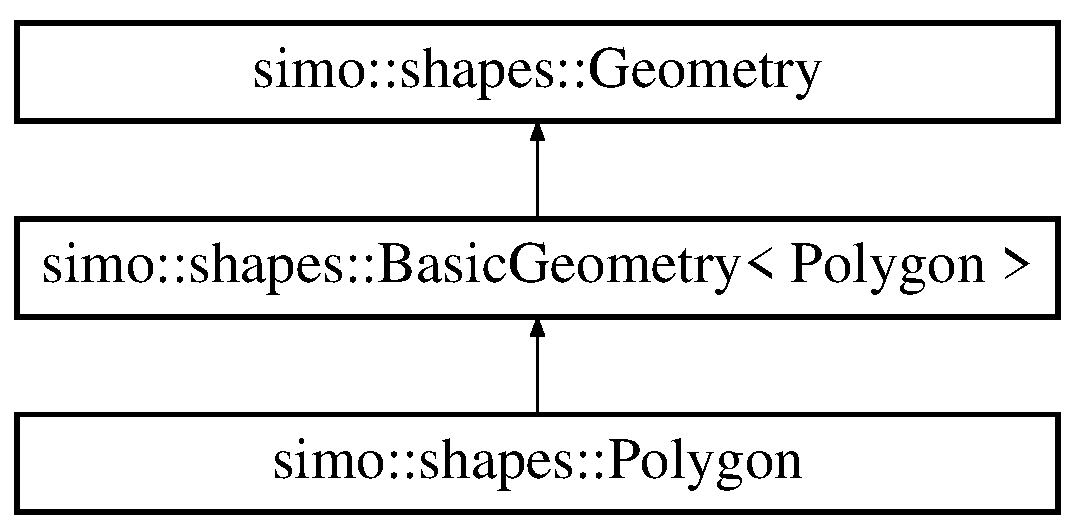
\includegraphics[height=3.000000cm]{classsimo_1_1shapes_1_1_polygon}
\end{center}
\end{figure}
\subsection*{Public Member Functions}
\begin{DoxyCompactItemize}
\item 
\hyperlink{classsimo_1_1shapes_1_1_polygon_a3069cb0007400aea8ae6ae2aa5041bfe}{Polygon} ()=default
\begin{DoxyCompactList}\small\item\em creates an empty \hyperlink{classsimo_1_1shapes_1_1_polygon}{Polygon} \end{DoxyCompactList}\item 
\hyperlink{classsimo_1_1shapes_1_1_polygon_a40b5518aefa6bb6992ec6bfc5ed90c2b}{Polygon} (const std\-::vector$<$ \hyperlink{classsimo_1_1shapes_1_1_point}{Point} $>$ \&shell)
\begin{DoxyCompactList}\small\item\em creates a \hyperlink{classsimo_1_1shapes_1_1_polygon}{Polygon} \end{DoxyCompactList}\item 
\hyperlink{classsimo_1_1shapes_1_1_polygon_a26336c46677a50f571dcd5651cccf869}{Polygon} (const std\-::vector$<$ \hyperlink{classsimo_1_1shapes_1_1_point}{Point} $>$ \&shell, const std\-::vector$<$ std\-::vector$<$ \hyperlink{classsimo_1_1shapes_1_1_point}{Point} $>$$>$ \&holes)
\begin{DoxyCompactList}\small\item\em creates a \hyperlink{classsimo_1_1shapes_1_1_polygon}{Polygon} \end{DoxyCompactList}\item 
std\-::string \hyperlink{classsimo_1_1shapes_1_1_polygon_adb65017c154a1907db5c7e70a721183e}{json} ()
\begin{DoxyCompactList}\small\item\em dumps the geojson representation of the \hyperlink{classsimo_1_1shapes_1_1_polygon}{Polygon} \end{DoxyCompactList}\item 
std\-::string \hyperlink{classsimo_1_1shapes_1_1_polygon_aac48a301f6b32faf9ffc1e42bd281857}{wkt} ()
\begin{DoxyCompactList}\small\item\em creates a \hyperlink{classsimo_1_1shapes_1_1_polygon}{Polygon} from a W\-K\-T string \end{DoxyCompactList}\end{DoxyCompactItemize}
\subsection*{Static Public Member Functions}
\begin{DoxyCompactItemize}
\item 
static \hyperlink{classsimo_1_1shapes_1_1_polygon}{Polygon} \hyperlink{classsimo_1_1shapes_1_1_polygon_a9fdf028143aa6849082458f9f4c95e4e}{from\-\_\-json} (const std\-::string \&)
\begin{DoxyCompactList}\small\item\em creates a \hyperlink{classsimo_1_1shapes_1_1_polygon}{Polygon} from a geojson string \end{DoxyCompactList}\item 
static \hyperlink{classsimo_1_1shapes_1_1_polygon}{Polygon} \hyperlink{classsimo_1_1shapes_1_1_polygon_a60178ce736c8cf87026d5730c73876cf}{from\-\_\-wkt} (const std\-::string \&)
\begin{DoxyCompactList}\small\item\em creates a \hyperlink{classsimo_1_1shapes_1_1_polygon}{Polygon} from a W\-K\-T string \end{DoxyCompactList}\end{DoxyCompactItemize}
\subsection*{Public Attributes}
\begin{DoxyCompactItemize}
\item 
\hypertarget{classsimo_1_1shapes_1_1_polygon_ab7f8d277bfe2342521ec9c35661ff692}{\hyperlink{classsimo_1_1shapes_1_1_linear_ring}{Linear\-Ring} \hyperlink{classsimo_1_1shapes_1_1_polygon_ab7f8d277bfe2342521ec9c35661ff692}{exterior}}\label{classsimo_1_1shapes_1_1_polygon_ab7f8d277bfe2342521ec9c35661ff692}

\begin{DoxyCompactList}\small\item\em linear ring that represents the shell of the polygon \end{DoxyCompactList}\item 
\hypertarget{classsimo_1_1shapes_1_1_polygon_a94f2f05198bd29714d9ecf6d60b83c2d}{std\-::vector$<$ \hyperlink{classsimo_1_1shapes_1_1_linear_ring}{Linear\-Ring} $>$ \hyperlink{classsimo_1_1shapes_1_1_polygon_a94f2f05198bd29714d9ecf6d60b83c2d}{interiors}}\label{classsimo_1_1shapes_1_1_polygon_a94f2f05198bd29714d9ecf6d60b83c2d}

\begin{DoxyCompactList}\small\item\em collection of linear rings that represent the holes of the polygon \end{DoxyCompactList}\end{DoxyCompactItemize}


\subsection{Detailed Description}


Definition at line 16 of file polygon.\-hpp.



\subsection{Constructor \& Destructor Documentation}
\hypertarget{classsimo_1_1shapes_1_1_polygon_a3069cb0007400aea8ae6ae2aa5041bfe}{\index{simo\-::shapes\-::\-Polygon@{simo\-::shapes\-::\-Polygon}!Polygon@{Polygon}}
\index{Polygon@{Polygon}!simo::shapes::Polygon@{simo\-::shapes\-::\-Polygon}}
\subsubsection[{Polygon}]{\setlength{\rightskip}{0pt plus 5cm}simo\-::shapes\-::\-Polygon\-::\-Polygon (
\begin{DoxyParamCaption}
{}
\end{DoxyParamCaption}
)\hspace{0.3cm}{\ttfamily [default]}}}\label{classsimo_1_1shapes_1_1_polygon_a3069cb0007400aea8ae6ae2aa5041bfe}


creates an empty \hyperlink{classsimo_1_1shapes_1_1_polygon}{Polygon} 

\begin{DoxySince}{Since}
0.\-0.\-1 
\end{DoxySince}
\hypertarget{classsimo_1_1shapes_1_1_polygon_a40b5518aefa6bb6992ec6bfc5ed90c2b}{\index{simo\-::shapes\-::\-Polygon@{simo\-::shapes\-::\-Polygon}!Polygon@{Polygon}}
\index{Polygon@{Polygon}!simo::shapes::Polygon@{simo\-::shapes\-::\-Polygon}}
\subsubsection[{Polygon}]{\setlength{\rightskip}{0pt plus 5cm}simo\-::shapes\-::\-Polygon\-::\-Polygon (
\begin{DoxyParamCaption}
\item[{const std\-::vector$<$ {\bf Point} $>$ \&}]{shell}
\end{DoxyParamCaption}
)\hspace{0.3cm}{\ttfamily [inline]}, {\ttfamily [explicit]}}}\label{classsimo_1_1shapes_1_1_polygon_a40b5518aefa6bb6992ec6bfc5ed90c2b}


creates a \hyperlink{classsimo_1_1shapes_1_1_polygon}{Polygon} 


\begin{DoxyParams}{Parameters}
{\em shell} & the shell of the polygon as a \hyperlink{classsimo_1_1shapes_1_1_point}{Point} sequence\\
\hline
\end{DoxyParams}
\begin{DoxySince}{Since}
0.\-0.\-1 
\end{DoxySince}


Definition at line 38 of file polygon.\-hpp.

\hypertarget{classsimo_1_1shapes_1_1_polygon_a26336c46677a50f571dcd5651cccf869}{\index{simo\-::shapes\-::\-Polygon@{simo\-::shapes\-::\-Polygon}!Polygon@{Polygon}}
\index{Polygon@{Polygon}!simo::shapes::Polygon@{simo\-::shapes\-::\-Polygon}}
\subsubsection[{Polygon}]{\setlength{\rightskip}{0pt plus 5cm}simo\-::shapes\-::\-Polygon\-::\-Polygon (
\begin{DoxyParamCaption}
\item[{const std\-::vector$<$ {\bf Point} $>$ \&}]{shell, }
\item[{const std\-::vector$<$ std\-::vector$<$ {\bf Point} $>$$>$ \&}]{holes}
\end{DoxyParamCaption}
)\hspace{0.3cm}{\ttfamily [inline]}}}\label{classsimo_1_1shapes_1_1_polygon_a26336c46677a50f571dcd5651cccf869}


creates a \hyperlink{classsimo_1_1shapes_1_1_polygon}{Polygon} 


\begin{DoxyParams}{Parameters}
{\em shell} & the shell of the polygon as a \hyperlink{classsimo_1_1shapes_1_1_point}{Point} sequence \\
\hline
{\em holes} & one or more collection of points, each representing a hole in the polygon\\
\hline
\end{DoxyParams}
\begin{DoxySince}{Since}
0.\-0.\-1 
\end{DoxySince}


Definition at line 54 of file polygon.\-hpp.



\subsection{Member Function Documentation}
\hypertarget{classsimo_1_1shapes_1_1_polygon_a9fdf028143aa6849082458f9f4c95e4e}{\index{simo\-::shapes\-::\-Polygon@{simo\-::shapes\-::\-Polygon}!from\-\_\-json@{from\-\_\-json}}
\index{from\-\_\-json@{from\-\_\-json}!simo::shapes::Polygon@{simo\-::shapes\-::\-Polygon}}
\subsubsection[{from\-\_\-json}]{\setlength{\rightskip}{0pt plus 5cm}static {\bf Polygon} simo\-::shapes\-::\-Polygon\-::from\-\_\-json (
\begin{DoxyParamCaption}
\item[{const std\-::string \&}]{}
\end{DoxyParamCaption}
)\hspace{0.3cm}{\ttfamily [inline]}, {\ttfamily [static]}}}\label{classsimo_1_1shapes_1_1_polygon_a9fdf028143aa6849082458f9f4c95e4e}


creates a \hyperlink{classsimo_1_1shapes_1_1_polygon}{Polygon} from a geojson string 


\begin{DoxyParams}{Parameters}
{\em json} & the geojson string \\
\hline
\end{DoxyParams}
\begin{DoxyReturn}{Returns}
a \hyperlink{classsimo_1_1shapes_1_1_polygon}{Polygon} object
\end{DoxyReturn}
\begin{DoxyNote}{Note}
R\-F\-C7946 \href{https://tools.ietf.org/html/rfc7946}{\tt https\-://tools.\-ietf.\-org/html/rfc7946}
\end{DoxyNote}
\begin{DoxySince}{Since}
0.\-0.\-1 
\end{DoxySince}


Definition at line 134 of file polygon.\-hpp.

\hypertarget{classsimo_1_1shapes_1_1_polygon_a60178ce736c8cf87026d5730c73876cf}{\index{simo\-::shapes\-::\-Polygon@{simo\-::shapes\-::\-Polygon}!from\-\_\-wkt@{from\-\_\-wkt}}
\index{from\-\_\-wkt@{from\-\_\-wkt}!simo::shapes::Polygon@{simo\-::shapes\-::\-Polygon}}
\subsubsection[{from\-\_\-wkt}]{\setlength{\rightskip}{0pt plus 5cm}static {\bf Polygon} simo\-::shapes\-::\-Polygon\-::from\-\_\-wkt (
\begin{DoxyParamCaption}
\item[{const std\-::string \&}]{}
\end{DoxyParamCaption}
)\hspace{0.3cm}{\ttfamily [inline]}, {\ttfamily [static]}}}\label{classsimo_1_1shapes_1_1_polygon_a60178ce736c8cf87026d5730c73876cf}


creates a \hyperlink{classsimo_1_1shapes_1_1_polygon}{Polygon} from a W\-K\-T string 


\begin{DoxyParams}{Parameters}
{\em wkt} & the W\-K\-T string \\
\hline
\end{DoxyParams}
\begin{DoxyReturn}{Returns}
a \hyperlink{classsimo_1_1shapes_1_1_polygon}{Polygon} object
\end{DoxyReturn}
\begin{DoxyNote}{Note}
W\-K\-T \href{https://en.wikipedia.org/wiki/Well-known_text_representation_of_geometry}{\tt https\-://en.\-wikipedia.\-org/wiki/\-Well-\/known\-\_\-text\-\_\-representation\-\_\-of\-\_\-geometry}
\end{DoxyNote}
\begin{DoxySince}{Since}
0.\-0.\-1 
\end{DoxySince}


Definition at line 163 of file polygon.\-hpp.

\hypertarget{classsimo_1_1shapes_1_1_polygon_adb65017c154a1907db5c7e70a721183e}{\index{simo\-::shapes\-::\-Polygon@{simo\-::shapes\-::\-Polygon}!json@{json}}
\index{json@{json}!simo::shapes::Polygon@{simo\-::shapes\-::\-Polygon}}
\subsubsection[{json}]{\setlength{\rightskip}{0pt plus 5cm}std\-::string simo\-::shapes\-::\-Polygon\-::json (
\begin{DoxyParamCaption}
{}
\end{DoxyParamCaption}
)\hspace{0.3cm}{\ttfamily [inline]}}}\label{classsimo_1_1shapes_1_1_polygon_adb65017c154a1907db5c7e70a721183e}


dumps the geojson representation of the \hyperlink{classsimo_1_1shapes_1_1_polygon}{Polygon} 

\begin{DoxyNote}{Note}
R\-F\-C7946 \href{https://tools.ietf.org/html/rfc7946}{\tt https\-://tools.\-ietf.\-org/html/rfc7946}
\end{DoxyNote}
\begin{DoxyReturn}{Returns}
a geojson string
\end{DoxyReturn}
\begin{DoxySince}{Since}
0.\-0.\-1 
\end{DoxySince}


Definition at line 148 of file polygon.\-hpp.

\hypertarget{classsimo_1_1shapes_1_1_polygon_aac48a301f6b32faf9ffc1e42bd281857}{\index{simo\-::shapes\-::\-Polygon@{simo\-::shapes\-::\-Polygon}!wkt@{wkt}}
\index{wkt@{wkt}!simo::shapes::Polygon@{simo\-::shapes\-::\-Polygon}}
\subsubsection[{wkt}]{\setlength{\rightskip}{0pt plus 5cm}std\-::string simo\-::shapes\-::\-Polygon\-::wkt (
\begin{DoxyParamCaption}
{}
\end{DoxyParamCaption}
)\hspace{0.3cm}{\ttfamily [inline]}}}\label{classsimo_1_1shapes_1_1_polygon_aac48a301f6b32faf9ffc1e42bd281857}


creates a \hyperlink{classsimo_1_1shapes_1_1_polygon}{Polygon} from a W\-K\-T string 


\begin{DoxyParams}{Parameters}
{\em wkt} & the W\-K\-T string \\
\hline
\end{DoxyParams}
\begin{DoxyReturn}{Returns}
a \hyperlink{classsimo_1_1shapes_1_1_polygon}{Polygon} object
\end{DoxyReturn}
\begin{DoxyNote}{Note}
W\-K\-T \href{https://en.wikipedia.org/wiki/Well-known_text_representation_of_geometry}{\tt https\-://en.\-wikipedia.\-org/wiki/\-Well-\/known\-\_\-text\-\_\-representation\-\_\-of\-\_\-geometry}
\end{DoxyNote}
\begin{DoxySince}{Since}
0.\-0.\-1 
\end{DoxySince}


Definition at line 178 of file polygon.\-hpp.



The documentation for this class was generated from the following file\-:\begin{DoxyCompactItemize}
\item 
/home/travis/build/pavelsimo/shapes/include/simo/geom/polygon.\-hpp\end{DoxyCompactItemize}

\hypertarget{classsimo_1_1shapes_1_1exceptions_1_1shapes__exception}{\section{simo\-:\-:shapes\-:\-:exceptions\-:\-:shapes\-\_\-exception Class Reference}
\label{classsimo_1_1shapes_1_1exceptions_1_1shapes__exception}\index{simo\-::shapes\-::exceptions\-::shapes\-\_\-exception@{simo\-::shapes\-::exceptions\-::shapes\-\_\-exception}}
}


base shapes exception  




{\ttfamily \#include $<$exceptions.\-hpp$>$}

Inheritance diagram for simo\-:\-:shapes\-:\-:exceptions\-:\-:shapes\-\_\-exception\-:\begin{figure}[H]
\begin{center}
\leavevmode
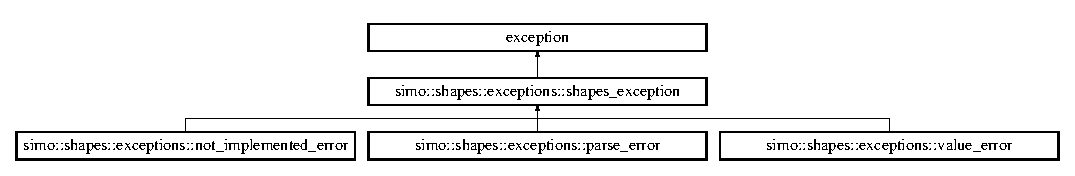
\includegraphics[height=1.917808cm]{classsimo_1_1shapes_1_1exceptions_1_1shapes__exception}
\end{center}
\end{figure}
\subsection*{Public Member Functions}
\begin{DoxyCompactItemize}
\item 
\hypertarget{classsimo_1_1shapes_1_1exceptions_1_1shapes__exception_a42d5526d2f6465814d1e74c4d79f30c1}{{\bfseries shapes\-\_\-exception} (const char $\ast$what)}\label{classsimo_1_1shapes_1_1exceptions_1_1shapes__exception_a42d5526d2f6465814d1e74c4d79f30c1}

\item 
\hypertarget{classsimo_1_1shapes_1_1exceptions_1_1shapes__exception_a61bf1548a63f7df164dbf2812a3fabe3}{const char $\ast$ {\bfseries what} () const noexceptoverride}\label{classsimo_1_1shapes_1_1exceptions_1_1shapes__exception_a61bf1548a63f7df164dbf2812a3fabe3}

\end{DoxyCompactItemize}
\subsection*{Protected Member Functions}
\begin{DoxyCompactItemize}
\item 
\hypertarget{classsimo_1_1shapes_1_1exceptions_1_1shapes__exception_a69e9e832d2b609f810d67f629d36d1ae}{void {\bfseries set\-\_\-reason} (const std\-::string \&reason)}\label{classsimo_1_1shapes_1_1exceptions_1_1shapes__exception_a69e9e832d2b609f810d67f629d36d1ae}

\end{DoxyCompactItemize}


\subsection{Detailed Description}
base shapes exception 

Definition at line 16 of file exceptions.\-hpp.



The documentation for this class was generated from the following file\-:\begin{DoxyCompactItemize}
\item 
/home/travis/build/pavelsimo/shapes/include/simo/exceptions.\-hpp\end{DoxyCompactItemize}

\hypertarget{classsimo_1_1shapes_1_1exceptions_1_1value__error}{\section{simo\-:\-:shapes\-:\-:exceptions\-:\-:value\-\_\-error Class Reference}
\label{classsimo_1_1shapes_1_1exceptions_1_1value__error}\index{simo\-::shapes\-::exceptions\-::value\-\_\-error@{simo\-::shapes\-::exceptions\-::value\-\_\-error}}
}


{\ttfamily \#include $<$exceptions.\-hpp$>$}

Inheritance diagram for simo\-:\-:shapes\-:\-:exceptions\-:\-:value\-\_\-error\-:\begin{figure}[H]
\begin{center}
\leavevmode
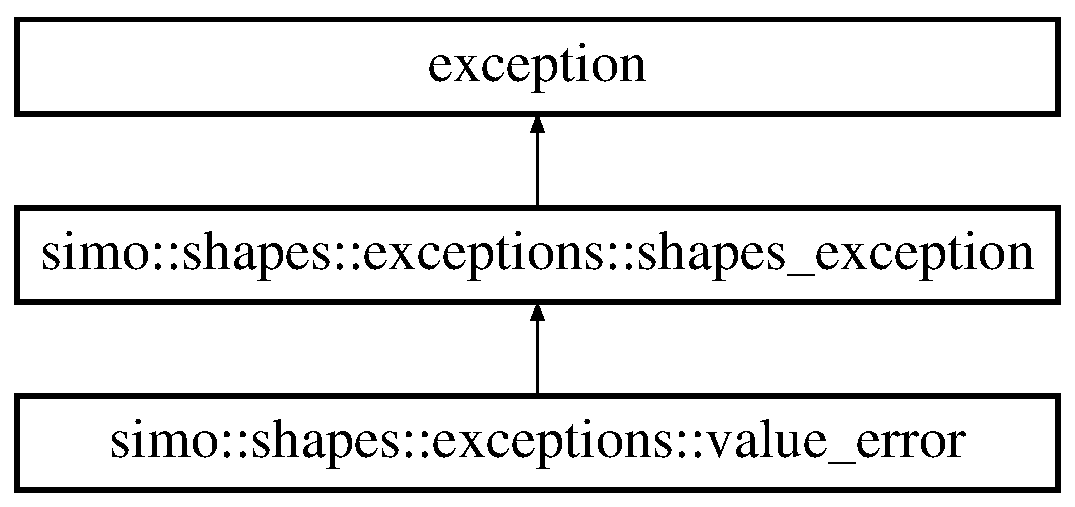
\includegraphics[height=3.000000cm]{classsimo_1_1shapes_1_1exceptions_1_1value__error}
\end{center}
\end{figure}
\subsection*{Public Member Functions}
\begin{DoxyCompactItemize}
\item 
\hypertarget{classsimo_1_1shapes_1_1exceptions_1_1value__error_a016a1db56ac487d44ee9bea79fe9e57e}{{\bfseries value\-\_\-error} (const std\-::string \&reason)}\label{classsimo_1_1shapes_1_1exceptions_1_1value__error_a016a1db56ac487d44ee9bea79fe9e57e}

\end{DoxyCompactItemize}
\subsection*{Additional Inherited Members}


\subsection{Detailed Description}
\begin{DoxyRefDesc}{Todo}
\item[\hyperlink{todo__todo000003}{Todo}](pavel) D\-O\-C\-U\-M\-E\-N\-T M\-E! \end{DoxyRefDesc}


Definition at line 72 of file exceptions.\-hpp.



The documentation for this class was generated from the following file\-:\begin{DoxyCompactItemize}
\item 
/home/travis/build/pavelsimo/shapes/include/simo/exceptions.\-hpp\end{DoxyCompactItemize}

\hypertarget{classsimo_1_1shapes_1_1wkt__lexer}{\section{simo\-:\-:shapes\-:\-:wkt\-\_\-lexer Class Reference}
\label{classsimo_1_1shapes_1_1wkt__lexer}\index{simo\-::shapes\-::wkt\-\_\-lexer@{simo\-::shapes\-::wkt\-\_\-lexer}}
}
\subsection*{Public Member Functions}
\begin{DoxyCompactItemize}
\item 
\hypertarget{classsimo_1_1shapes_1_1wkt__lexer_ad84a7fd2b5aadab778b25e28f8e5ab3d}{{\bfseries wkt\-\_\-lexer} (const char $\ast$source)}\label{classsimo_1_1shapes_1_1wkt__lexer_ad84a7fd2b5aadab778b25e28f8e5ab3d}

\item 
int \hyperlink{classsimo_1_1shapes_1_1wkt__lexer_a7473195841ab0423102576ef7c392edb}{scan} ()
\item 
\hypertarget{classsimo_1_1shapes_1_1wkt__lexer_a32267afbdbcd9110f561e99d9dd6dbda}{std\-::string {\bfseries get\-\_\-token} () const }\label{classsimo_1_1shapes_1_1wkt__lexer_a32267afbdbcd9110f561e99d9dd6dbda}

\end{DoxyCompactItemize}


\subsection{Detailed Description}


Definition at line 11 of file wkt\-\_\-lexer.\-hpp.



\subsection{Member Function Documentation}
\hypertarget{classsimo_1_1shapes_1_1wkt__lexer_a7473195841ab0423102576ef7c392edb}{\index{simo\-::shapes\-::wkt\-\_\-lexer@{simo\-::shapes\-::wkt\-\_\-lexer}!scan@{scan}}
\index{scan@{scan}!simo::shapes::wkt_lexer@{simo\-::shapes\-::wkt\-\_\-lexer}}
\subsubsection[{scan}]{\setlength{\rightskip}{0pt plus 5cm}int simo\-::shapes\-::wkt\-\_\-lexer\-::scan (
\begin{DoxyParamCaption}
{}
\end{DoxyParamCaption}
)\hspace{0.3cm}{\ttfamily [inline]}}}\label{classsimo_1_1shapes_1_1wkt__lexer_a7473195841ab0423102576ef7c392edb}
pointer for backtracking information 

Definition at line 22 of file wkt\-\_\-lexer.\-hpp.



The documentation for this class was generated from the following file\-:\begin{DoxyCompactItemize}
\item 
/home/travis/build/pavelsimo/shapes/include/simo/io/wkt\-\_\-lexer.\-hpp\end{DoxyCompactItemize}

\hypertarget{classsimo_1_1shapes_1_1wkt__reader}{\section{simo\-:\-:shapes\-:\-:wkt\-\_\-reader Class Reference}
\label{classsimo_1_1shapes_1_1wkt__reader}\index{simo\-::shapes\-::wkt\-\_\-reader@{simo\-::shapes\-::wkt\-\_\-reader}}
}
\subsection*{Public Member Functions}
\begin{DoxyCompactItemize}
\item 
\hyperlink{classsimo_1_1shapes_1_1wkt__reader_a140190108a9314b118e271f251d5e3d8}{wkt\-\_\-reader} ()
\begin{DoxyCompactList}\small\item\em creates a W\-K\-T reader \end{DoxyCompactList}\item 
\hypertarget{classsimo_1_1shapes_1_1wkt__reader_a495f804e3972958ec98bfe00985cde2c}{\hyperlink{classsimo_1_1shapes_1_1wkt__reader_a495f804e3972958ec98bfe00985cde2c}{$\sim$wkt\-\_\-reader} ()}\label{classsimo_1_1shapes_1_1wkt__reader_a495f804e3972958ec98bfe00985cde2c}

\begin{DoxyCompactList}\small\item\em \hyperlink{classsimo_1_1shapes_1_1wkt__reader}{wkt\-\_\-reader} destructor \end{DoxyCompactList}\item 
\hyperlink{structsimo_1_1shapes_1_1wkt__result}{wkt\-\_\-result} \hyperlink{classsimo_1_1shapes_1_1wkt__reader_a2975dda35cd727ed6f1ad338d0a58861}{read} (const char $\ast$wkt)
\begin{DoxyCompactList}\small\item\em parse the given wkt string \end{DoxyCompactList}\end{DoxyCompactItemize}


\subsection{Detailed Description}


Definition at line 13 of file wkt\-\_\-reader.\-hpp.



\subsection{Constructor \& Destructor Documentation}
\hypertarget{classsimo_1_1shapes_1_1wkt__reader_a140190108a9314b118e271f251d5e3d8}{\index{simo\-::shapes\-::wkt\-\_\-reader@{simo\-::shapes\-::wkt\-\_\-reader}!wkt\-\_\-reader@{wkt\-\_\-reader}}
\index{wkt\-\_\-reader@{wkt\-\_\-reader}!simo::shapes::wkt_reader@{simo\-::shapes\-::wkt\-\_\-reader}}
\subsubsection[{wkt\-\_\-reader}]{\setlength{\rightskip}{0pt plus 5cm}simo\-::shapes\-::wkt\-\_\-reader\-::wkt\-\_\-reader (
\begin{DoxyParamCaption}
{}
\end{DoxyParamCaption}
)\hspace{0.3cm}{\ttfamily [inline]}}}\label{classsimo_1_1shapes_1_1wkt__reader_a140190108a9314b118e271f251d5e3d8}


creates a W\-K\-T reader 

\begin{DoxySince}{Since}
0.\-0.\-1 
\end{DoxySince}


Definition at line 21 of file wkt\-\_\-reader.\-hpp.



\subsection{Member Function Documentation}
\hypertarget{classsimo_1_1shapes_1_1wkt__reader_a2975dda35cd727ed6f1ad338d0a58861}{\index{simo\-::shapes\-::wkt\-\_\-reader@{simo\-::shapes\-::wkt\-\_\-reader}!read@{read}}
\index{read@{read}!simo::shapes::wkt_reader@{simo\-::shapes\-::wkt\-\_\-reader}}
\subsubsection[{read}]{\setlength{\rightskip}{0pt plus 5cm}{\bf wkt\-\_\-result} simo\-::shapes\-::wkt\-\_\-reader\-::read (
\begin{DoxyParamCaption}
\item[{const char $\ast$}]{wkt}
\end{DoxyParamCaption}
)\hspace{0.3cm}{\ttfamily [inline]}}}\label{classsimo_1_1shapes_1_1wkt__reader_a2975dda35cd727ed6f1ad338d0a58861}


parse the given wkt string 


\begin{DoxyParams}{Parameters}
{\em wkt} & the wkt string \\
\hline
\end{DoxyParams}
\begin{DoxyReturn}{Returns}
\hyperlink{structsimo_1_1shapes_1_1wkt__result}{wkt\-\_\-result} object
\end{DoxyReturn}
\begin{DoxySince}{Since}
0.\-0.\-1 
\end{DoxySince}


Definition at line 40 of file wkt\-\_\-reader.\-hpp.



The documentation for this class was generated from the following file\-:\begin{DoxyCompactItemize}
\item 
/home/travis/build/pavelsimo/shapes/include/simo/io/wkt\-\_\-reader.\-hpp\end{DoxyCompactItemize}

\hypertarget{structsimo_1_1shapes_1_1wkt__result}{\section{simo\-:\-:shapes\-:\-:wkt\-\_\-result Struct Reference}
\label{structsimo_1_1shapes_1_1wkt__result}\index{simo\-::shapes\-::wkt\-\_\-result@{simo\-::shapes\-::wkt\-\_\-result}}
}
\subsection*{Public Attributes}
\begin{DoxyCompactItemize}
\item 
\hypertarget{structsimo_1_1shapes_1_1wkt__result_ad21b447b14cd0e0e5abcf0dab6541405}{int {\bfseries parser\-\_\-error}}\label{structsimo_1_1shapes_1_1wkt__result_ad21b447b14cd0e0e5abcf0dab6541405}

\item 
\hypertarget{structsimo_1_1shapes_1_1wkt__result_aca8a845a61afb6eb33bb20e4c955ae19}{Dimension\-Type {\bfseries dim}}\label{structsimo_1_1shapes_1_1wkt__result_aca8a845a61afb6eb33bb20e4c955ae19}

\item 
\hypertarget{structsimo_1_1shapes_1_1wkt__result_a59af624bbd0230c451cebc3f264d3638}{int {\bfseries ndim}}\label{structsimo_1_1shapes_1_1wkt__result_a59af624bbd0230c451cebc3f264d3638}

\item 
\hypertarget{structsimo_1_1shapes_1_1wkt__result_a9452d4f908125eef6e6d20a977a314dd}{std\-::vector$<$ double $>$ {\bfseries coords}}\label{structsimo_1_1shapes_1_1wkt__result_a9452d4f908125eef6e6d20a977a314dd}

\item 
\hypertarget{structsimo_1_1shapes_1_1wkt__result_a54483bd061e9e29ca75bfb3da2dee955}{std\-::vector$<$ std\-::size\-\_\-t $>$ {\bfseries offsets}}\label{structsimo_1_1shapes_1_1wkt__result_a54483bd061e9e29ca75bfb3da2dee955}

\end{DoxyCompactItemize}


\subsection{Detailed Description}


Definition at line 10 of file wkt\-\_\-parser.\-hpp.



The documentation for this struct was generated from the following file\-:\begin{DoxyCompactItemize}
\item 
/home/travis/build/pavelsimo/shapes/include/simo/io/wkt\-\_\-parser.\-hpp\end{DoxyCompactItemize}

\hypertarget{union_y_y_m_i_n_o_r_t_y_p_e}{\section{Y\-Y\-M\-I\-N\-O\-R\-T\-Y\-P\-E Union Reference}
\label{union_y_y_m_i_n_o_r_t_y_p_e}\index{Y\-Y\-M\-I\-N\-O\-R\-T\-Y\-P\-E@{Y\-Y\-M\-I\-N\-O\-R\-T\-Y\-P\-E}}
}
\subsection*{Public Attributes}
\begin{DoxyCompactItemize}
\item 
\hypertarget{union_y_y_m_i_n_o_r_t_y_p_e_a6cec97309f473b42b70a9738d7cbd5ba}{int {\bfseries yyinit}}\label{union_y_y_m_i_n_o_r_t_y_p_e_a6cec97309f473b42b70a9738d7cbd5ba}

\item 
\hypertarget{union_y_y_m_i_n_o_r_t_y_p_e_a8cb8fd685f7268dccdcb7bdb80308242}{Parse\-T\-O\-K\-E\-N\-T\-Y\-P\-E {\bfseries yy0}}\label{union_y_y_m_i_n_o_r_t_y_p_e_a8cb8fd685f7268dccdcb7bdb80308242}

\end{DoxyCompactItemize}


\subsection{Detailed Description}


Definition at line 77 of file wkt\-\_\-parser.\-c.



The documentation for this union was generated from the following file\-:\begin{DoxyCompactItemize}
\item 
/home/travis/build/pavelsimo/shapes/include/simo/io/wkt\-\_\-parser.\-c\end{DoxyCompactItemize}

\hypertarget{structyy_parser}{\section{yy\-Parser Struct Reference}
\label{structyy_parser}\index{yy\-Parser@{yy\-Parser}}
}
\subsection*{Public Attributes}
\begin{DoxyCompactItemize}
\item 
\hypertarget{structyy_parser_a19abcf4780515fd2debd1ce7a2e29f95}{int {\bfseries yyidx}}\label{structyy_parser_a19abcf4780515fd2debd1ce7a2e29f95}

\item 
\hypertarget{structyy_parser_ac0350933aa515a3a756dfa742d04ee59}{int {\bfseries yyerrcnt}}\label{structyy_parser_ac0350933aa515a3a756dfa742d04ee59}

\item 
\hypertarget{structyy_parser_a269e4ebdc22c0b9102a8e29eebbdc201}{Parse\-A\-R\-G\-\_\-\-S\-D\-E\-C\-L \hyperlink{structyy_stack_entry}{yy\-Stack\-Entry} {\bfseries yystack} \mbox{[}Y\-Y\-S\-T\-A\-C\-K\-D\-E\-P\-T\-H\mbox{]}}\label{structyy_parser_a269e4ebdc22c0b9102a8e29eebbdc201}

\end{DoxyCompactItemize}


\subsection{Detailed Description}


Definition at line 231 of file wkt\-\_\-parser.\-c.



The documentation for this struct was generated from the following file\-:\begin{DoxyCompactItemize}
\item 
/home/travis/build/pavelsimo/shapes/include/simo/io/wkt\-\_\-parser.\-c\end{DoxyCompactItemize}

\hypertarget{structyy_stack_entry}{\section{yy\-Stack\-Entry Struct Reference}
\label{structyy_stack_entry}\index{yy\-Stack\-Entry@{yy\-Stack\-Entry}}
}
\subsection*{Public Attributes}
\begin{DoxyCompactItemize}
\item 
\hypertarget{structyy_stack_entry_a108164609c2e841577cc3533d8f0180d}{Y\-Y\-A\-C\-T\-I\-O\-N\-T\-Y\-P\-E {\bfseries stateno}}\label{structyy_stack_entry_a108164609c2e841577cc3533d8f0180d}

\item 
\hypertarget{structyy_stack_entry_a7624d02bcf945d48068f4c383551725c}{Y\-Y\-C\-O\-D\-E\-T\-Y\-P\-E {\bfseries major}}\label{structyy_stack_entry_a7624d02bcf945d48068f4c383551725c}

\item 
\hypertarget{structyy_stack_entry_a024e1e64bce5945080629a2dd8d1bb4f}{\hyperlink{union_y_y_m_i_n_o_r_t_y_p_e}{Y\-Y\-M\-I\-N\-O\-R\-T\-Y\-P\-E} {\bfseries minor}}\label{structyy_stack_entry_a024e1e64bce5945080629a2dd8d1bb4f}

\end{DoxyCompactItemize}


\subsection{Detailed Description}


Definition at line 220 of file wkt\-\_\-parser.\-c.



The documentation for this struct was generated from the following file\-:\begin{DoxyCompactItemize}
\item 
/home/travis/build/pavelsimo/shapes/include/simo/io/wkt\-\_\-parser.\-c\end{DoxyCompactItemize}

%--- End generated contents ---

% Index
\newpage
\phantomsection
\addcontentsline{toc}{chapter}{Index}
\printindex

\end{document}
